% TeX encoding = utf8
% TeX spellcheck = pl_PL 
\documentclass[a4paper, 11pt]{article}
\usepackage[utf8]{inputenc}
\usepackage[polish]{babel}
\usepackage{polski}
\usepackage{float}
\usepackage{graphicx}
\usepackage{listings}
\usepackage{amsfonts}
\usepackage{geometry}
\usepackage{multicol}
\usepackage{latexsym}
\usepackage{enumerate}
\usepackage{hyperref}
\usepackage{wrapfig}
\usepackage{color} %red, green, blue, yellow, cyan, magenta, black, white
\definecolor{mygreen}{RGB}{28,172,0} % color values Red, Green, Blue
\definecolor{mylilas}{RGB}{170,55,241}

\author{Kamil Foryszewski}
\title{Modelowanie i identyfkacja - projekt I, zadanie 9}
\frenchspacing

\newgeometry{tmargin=2cm, bmargin=2cm, lmargin=2cm, rmargin=2cm}
\pagestyle{empty}


\begin{document}

\lstset{language=Matlab,%
    basicstyle=\color{red},
    breaklines=true,%
    morekeywords={matlab2tikz},
    keywordstyle=\color{blue},%
    morekeywords=[2]{1}, keywordstyle=[2]{\color{black}},
    identifierstyle=\color{black},%
    stringstyle=\color{mylilas},%
    commentstyle=\color{mygreen},%
    showstringspaces=false,
    numbers=right,%
    numberstyle={ \color{black}},% size of the numbers
    numbersep=5pt, % this defines how far the numbers are from the text
    emph=[1]{for,endfor,endwhile,endfunction,endif,break},emphstyle=[1]\color{blue}, %some words to emphasise
    emph=[2]{,.}, emphstyle=[2]\color{yellow},%
}

\maketitle
\tableofcontents

\section{Dynamiczny model ciągły}
\subsection{Równanie modelu w przestrzeni stanu}
Obiekt dynamiczny opisany jest modelem ciągłym w przestrzeni stanu: 
\\

$\dot{x}_1 = -\frac{T_{1}-T_{2}}{T_{1}T_{2}}x_{1}(t) +x_{2}(t)$
\\

$\dot{x}_2 = -\frac{1}{T_{1}T_{2}}x_{1}(t) + \frac{K}{T_{1}T_{2}}(\alpha_{1}u(t) + \alpha_{2}u^2(t) + \alpha_{3}u^3(t) + \alpha_{4}u^4(t))$
\\

$y(t) = x_{1}(t)$
\\
\\
Gdzie : \\

$K  = 5.5, T_1 = 7, T_2 = 7, \alpha_1 = 0.19, \alpha_2 = -0.05, \alpha_3 = -0.95, \alpha_4 = -0.45,$
\\

Sygnał sterujący spałnia warunek $-1 \leq u \leq 1$
\\
\\
Po podstawieniu: 
\\

$\dot{x}_1 = -0.285714286x_{1}(t) +x_{2}(t)$
\\

$\dot{x}_2 = - 0.020408163x_{1}(t) - 0.021326531u(t) - 0.005612245u^2(t) - 0.106632653u^3(t) - 0.050510204u^4(t)$
\\

$y(t) = x_{1}(t)$
\\
\\
\subsection{Reprezentacja graficzna dynamicznego modelu ciągłego}
\begin{figure}[ht]
\centering
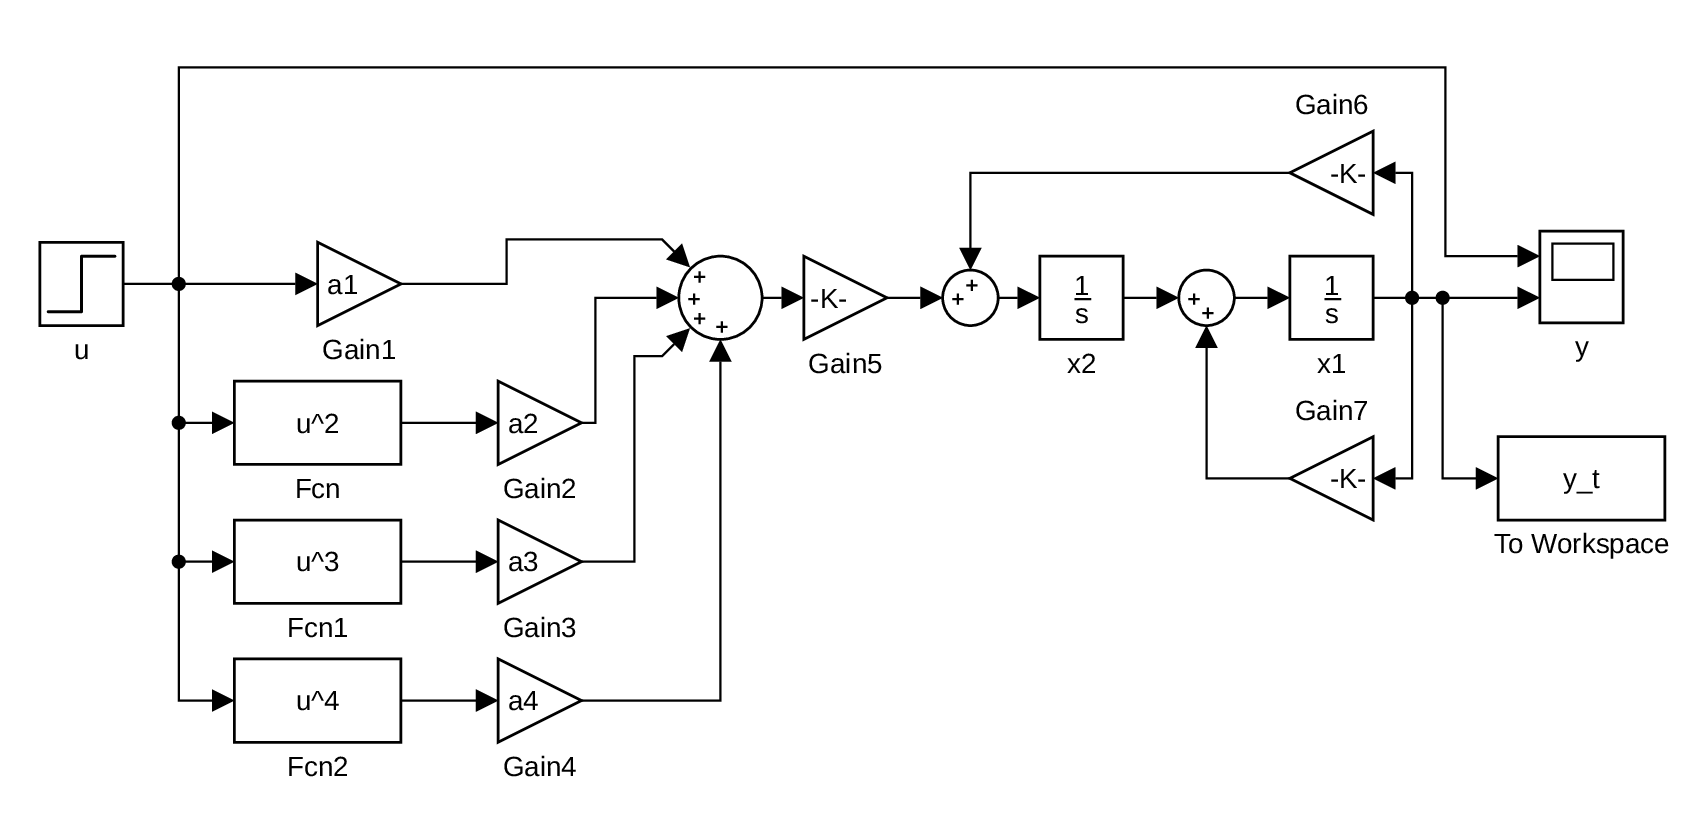
\includegraphics[scale=0.28]{dynamiczny_model_ciagly.png}
\caption{Reprezentacja graficzna dynamicznego modelu ciągłego }
\end{figure}


\section{Dynamiczny model dyskretny}

\subsection{Wyprowadzenie równania dynamicznego modelu dyskretnego}

Korzystając z metody aproksymacji wstecznej Eulera: 
\\

$\frac{x_1(k)- x_1(k-1)}{T_p} = -0.285714286x_1(k-1) +x_2(k-1)$
\\

$\frac{x_2(k)- x_2(k-1)}{T_p} = - 0.020408163x_1(k-1) - 0.021326531u(k-1) - 0.005612245u^2(k-1)\\
	\indent	- 0.106632653u^3(k-1) - 0.050510204u^4(k-1)$
\\

$y(k) = x_1(k)$
\\
\\
Po uproszczeniu: 
\\

$x_1(k) =(-0.285714286T_p+1)x_1(k-1)+T_px_2(k-1) $
\\

$x_2(k) = - 0.020408163T_px_1(k-1) + x_2(k-1) + T_p(-0.021326531u(k-1)-0.005612245u^2(k-1)\\
	\indent	- 0.106632653u^3(k-1)-0.050510204u^4(k-1))$
\\

$y(k) = x_1(k)$
\\
\\
W zapisie symbolicznym:
\\

$x_1(k) =(1-\frac{(T_1 + T_2)T_p}{T_1T_2})x_1(k-1)+T_px_2(k-1) $
\\

$x_2(k) = - \frac{T_p}{T_1T_2}x_1(k-1) + x_2(k-1) + T_p(\alpha_1u(k-1)+\alpha_2u^2(k-1)\\
	\indent	+ \alpha_3u^3(k-1)+\alpha_4u^4(k-1))$
\\

$y(k) = x_1(k)$
\\
\\
Gdzie : \\

$K  = 5.5, T_1 = 7, T_2 = 7, \alpha_1 = 0.19, \alpha_2 = -0.05, \alpha_3 = -0.95, \alpha_4 = -0.45, T_p$ - krok czasowy
\\


\subsection{Reprezentacja graficzna dynamicznego modelu dyskretnego}

\begin{figure}[ht]
\centering
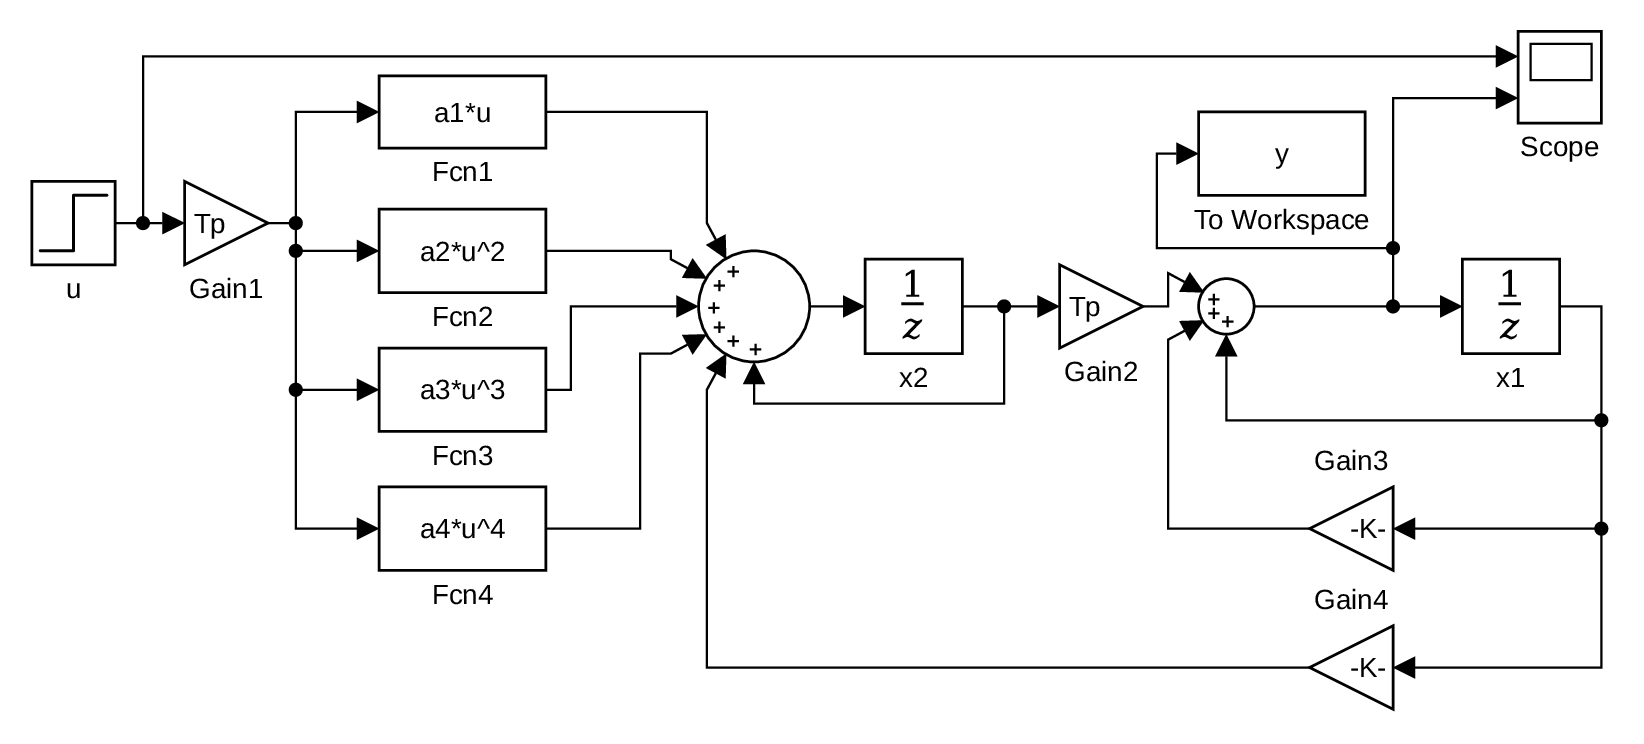
\includegraphics[scale=0.28]{dynamiczny_model_dyskretny.png}
\caption{Reprezentacja graficzna dynamicznego modelu dyskretnego}
\end{figure}

\section{Symulacje dynamicznego modelu ciągłego i dyskretnego}
\subsection{$T_p = 0.1$}
\begin{figure}[H]
\centering
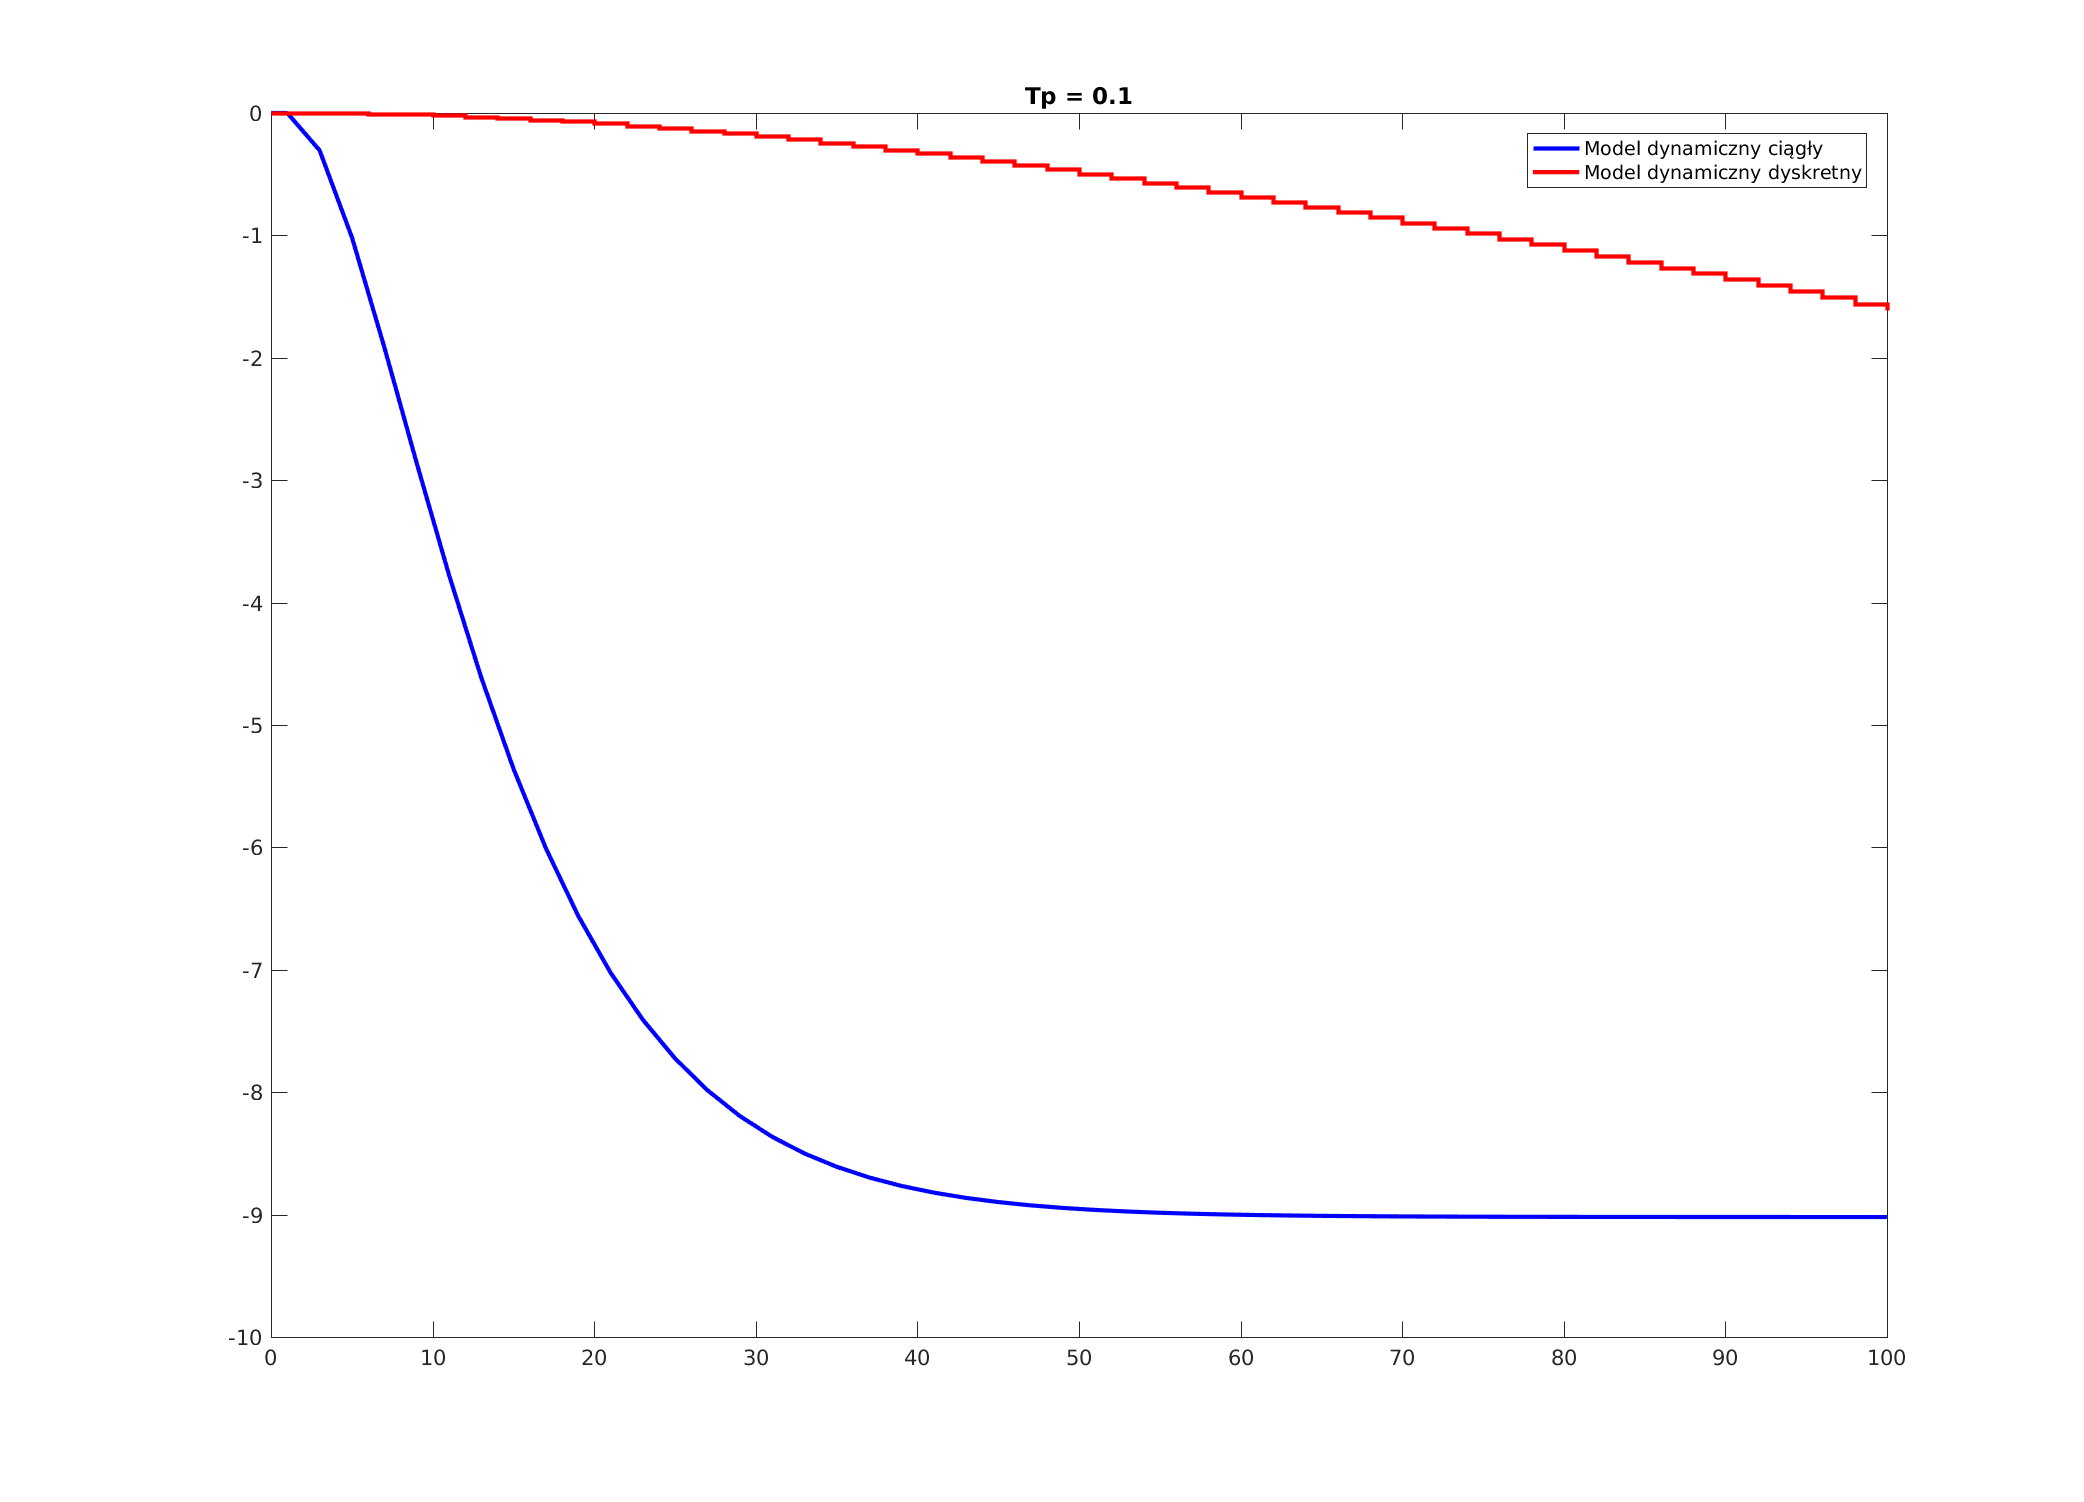
\includegraphics[scale=0.45]{tp_01.png}
\end{figure}
\subsection{$T_p = 0.25$}
\begin{figure}[H]
\centering
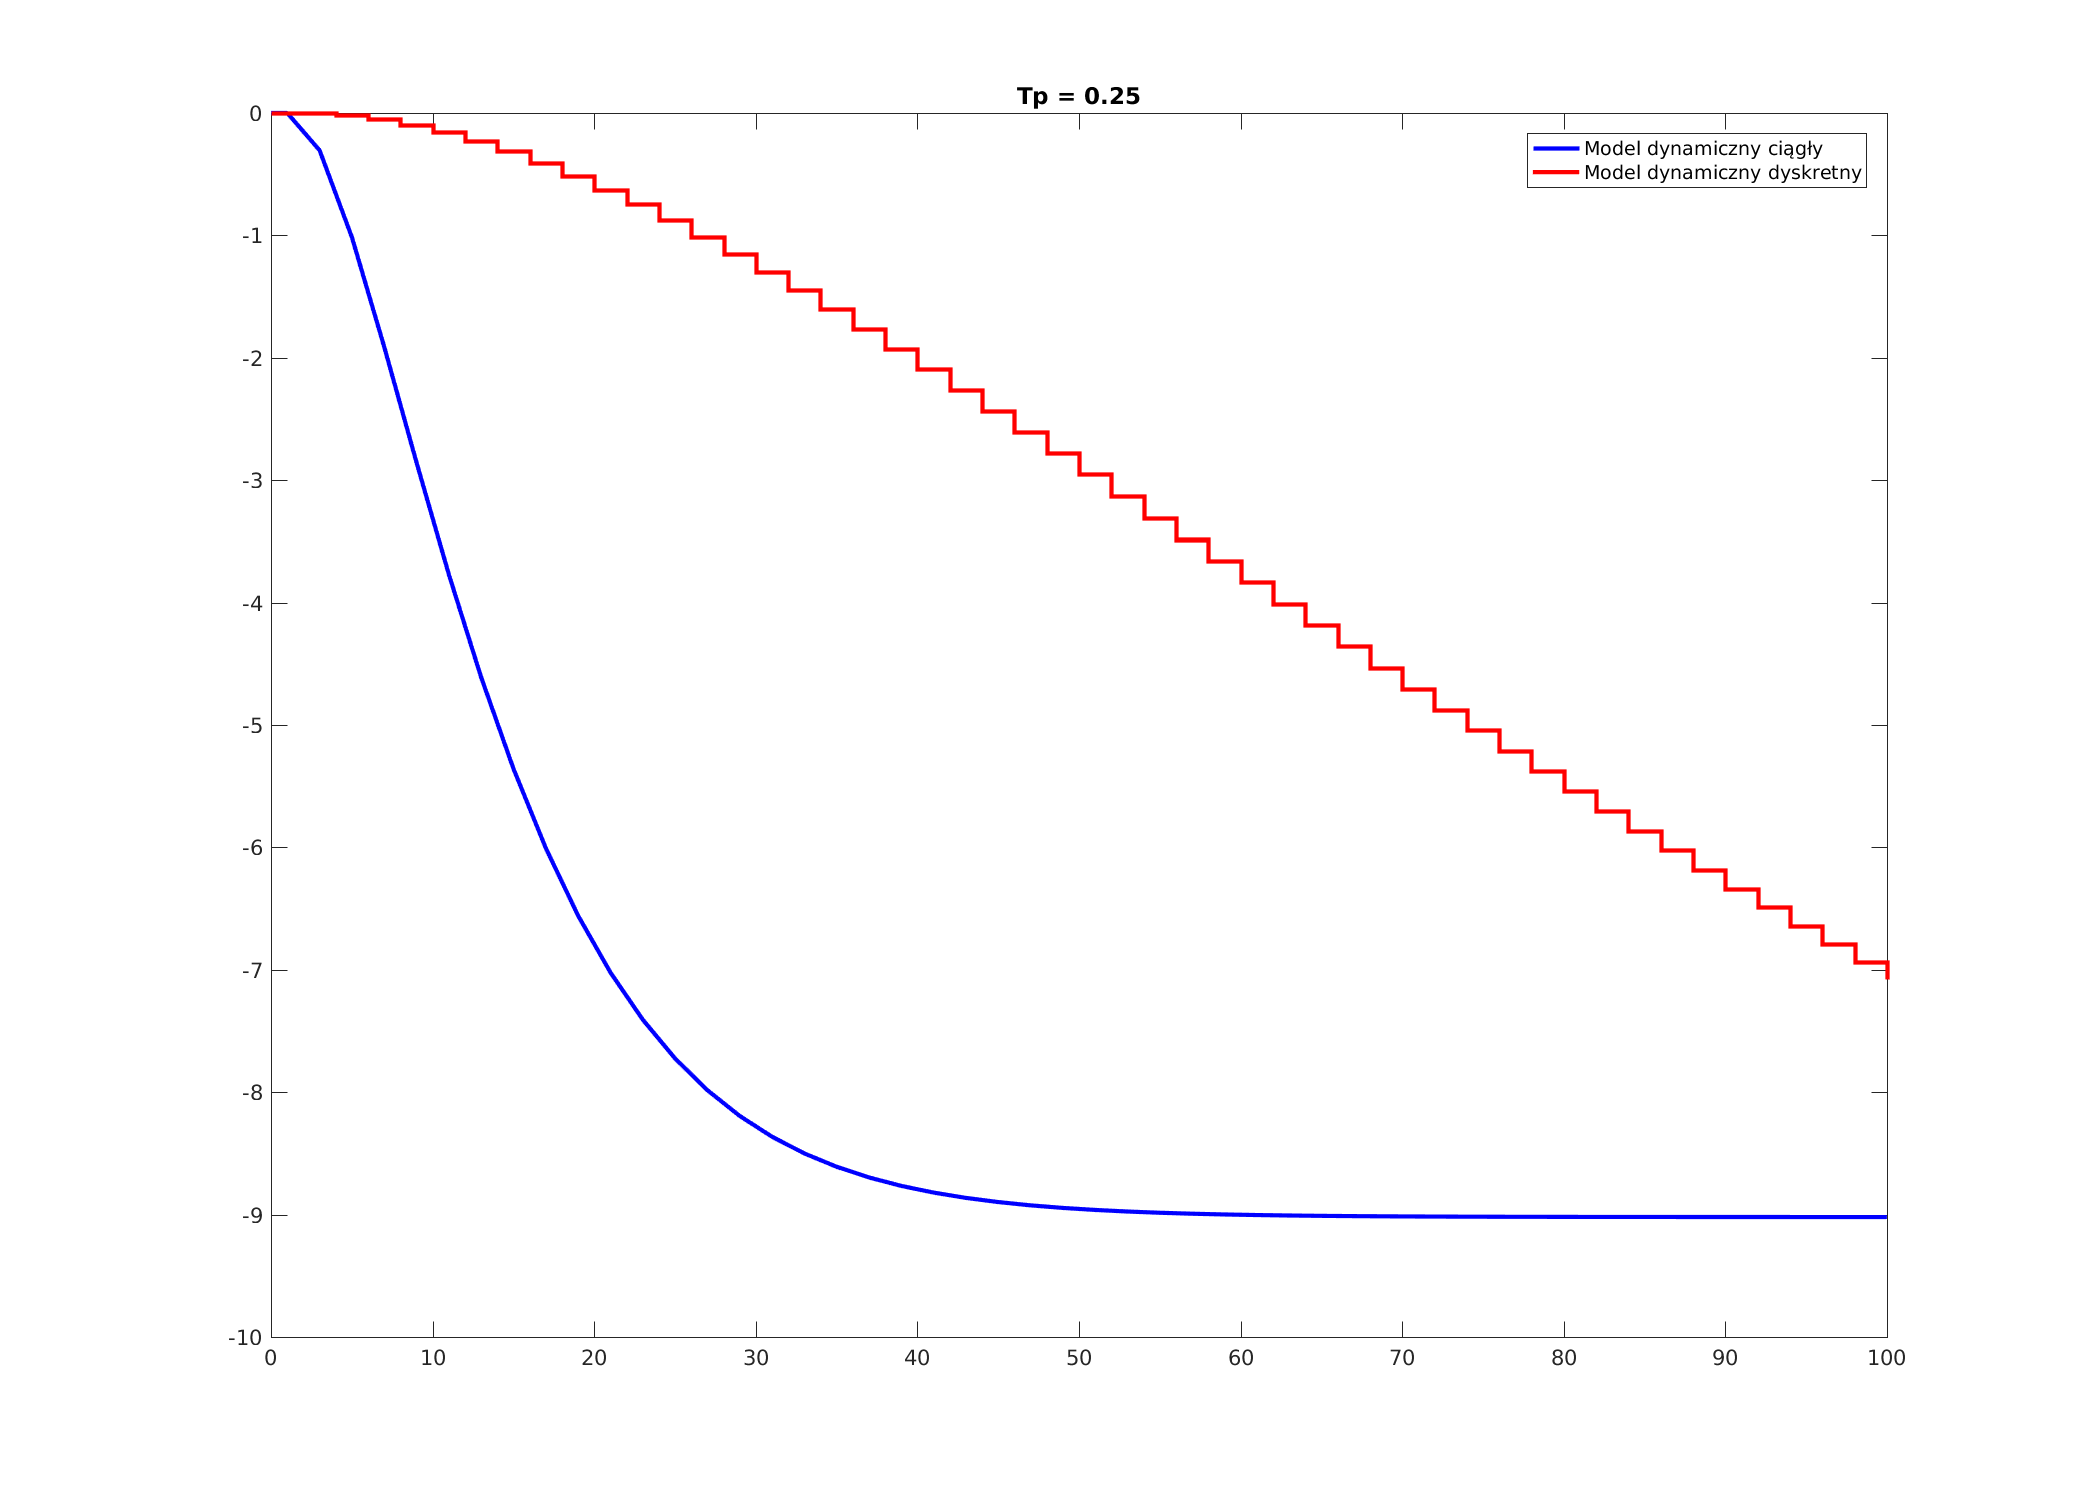
\includegraphics[scale=0.45]{tp_025.png}
\end{figure}

\subsection{$T_p = 0.5$}
\begin{figure}[H]
\centering
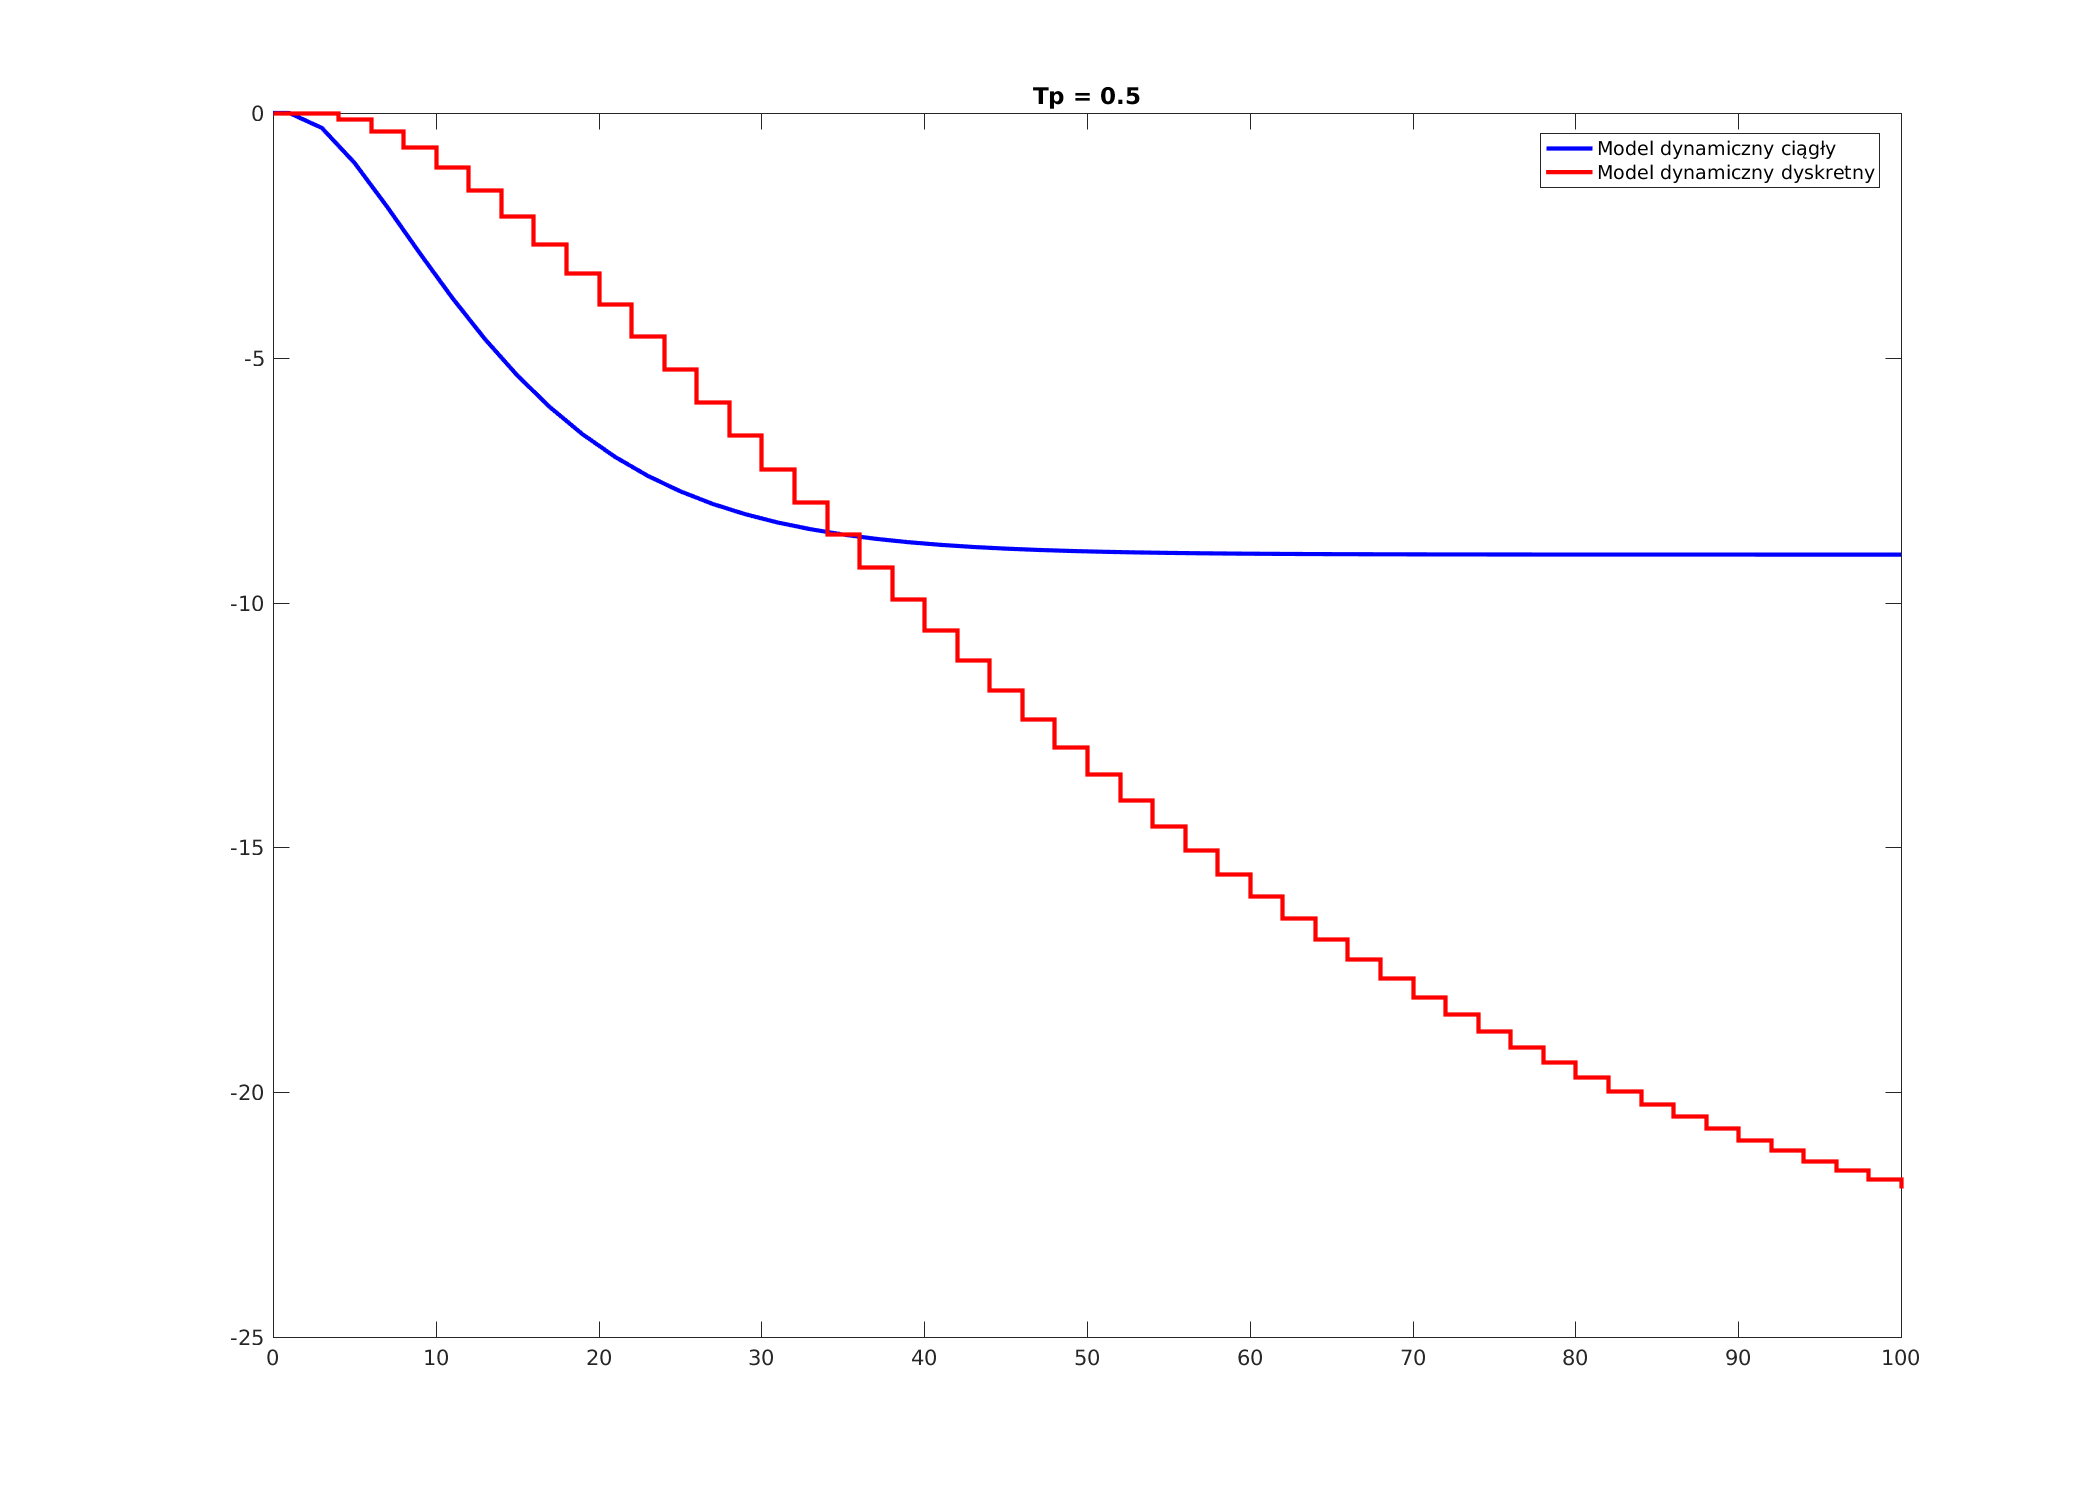
\includegraphics[scale=0.45]{tp_05.png}
\end{figure}

\subsection{$T_p = 1$}
\begin{figure}[H]
\centering
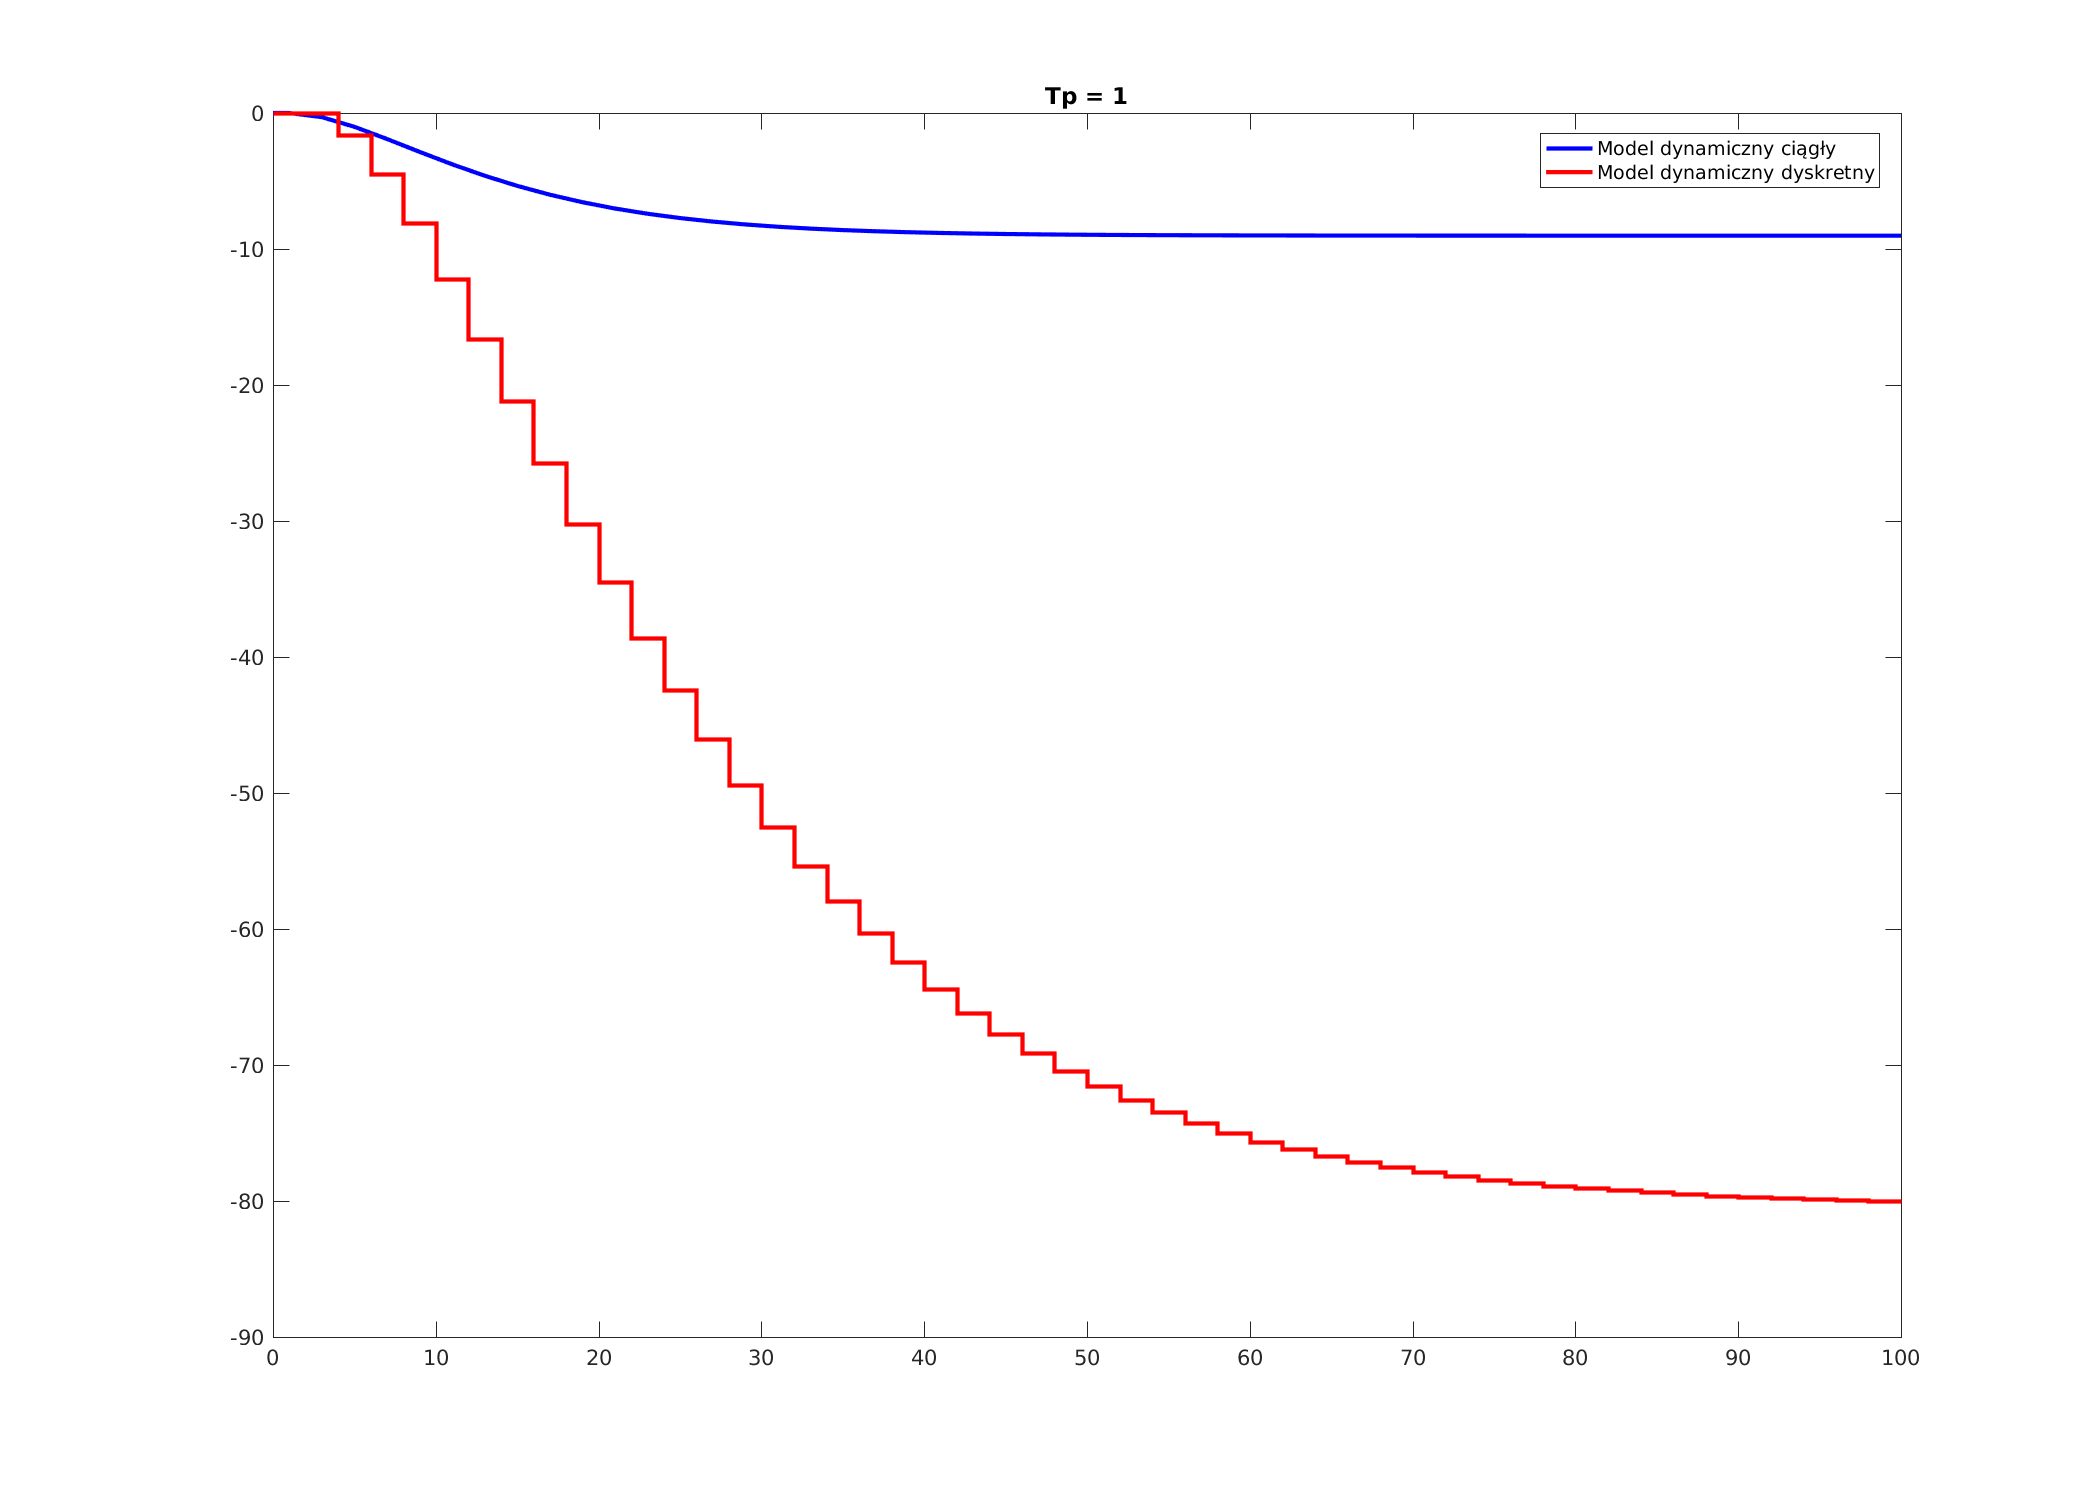
\includegraphics[scale=0.45]{tp_1.png}
\end{figure}

\subsection{$T_p = 2$}
\begin{figure}[H]
\centering
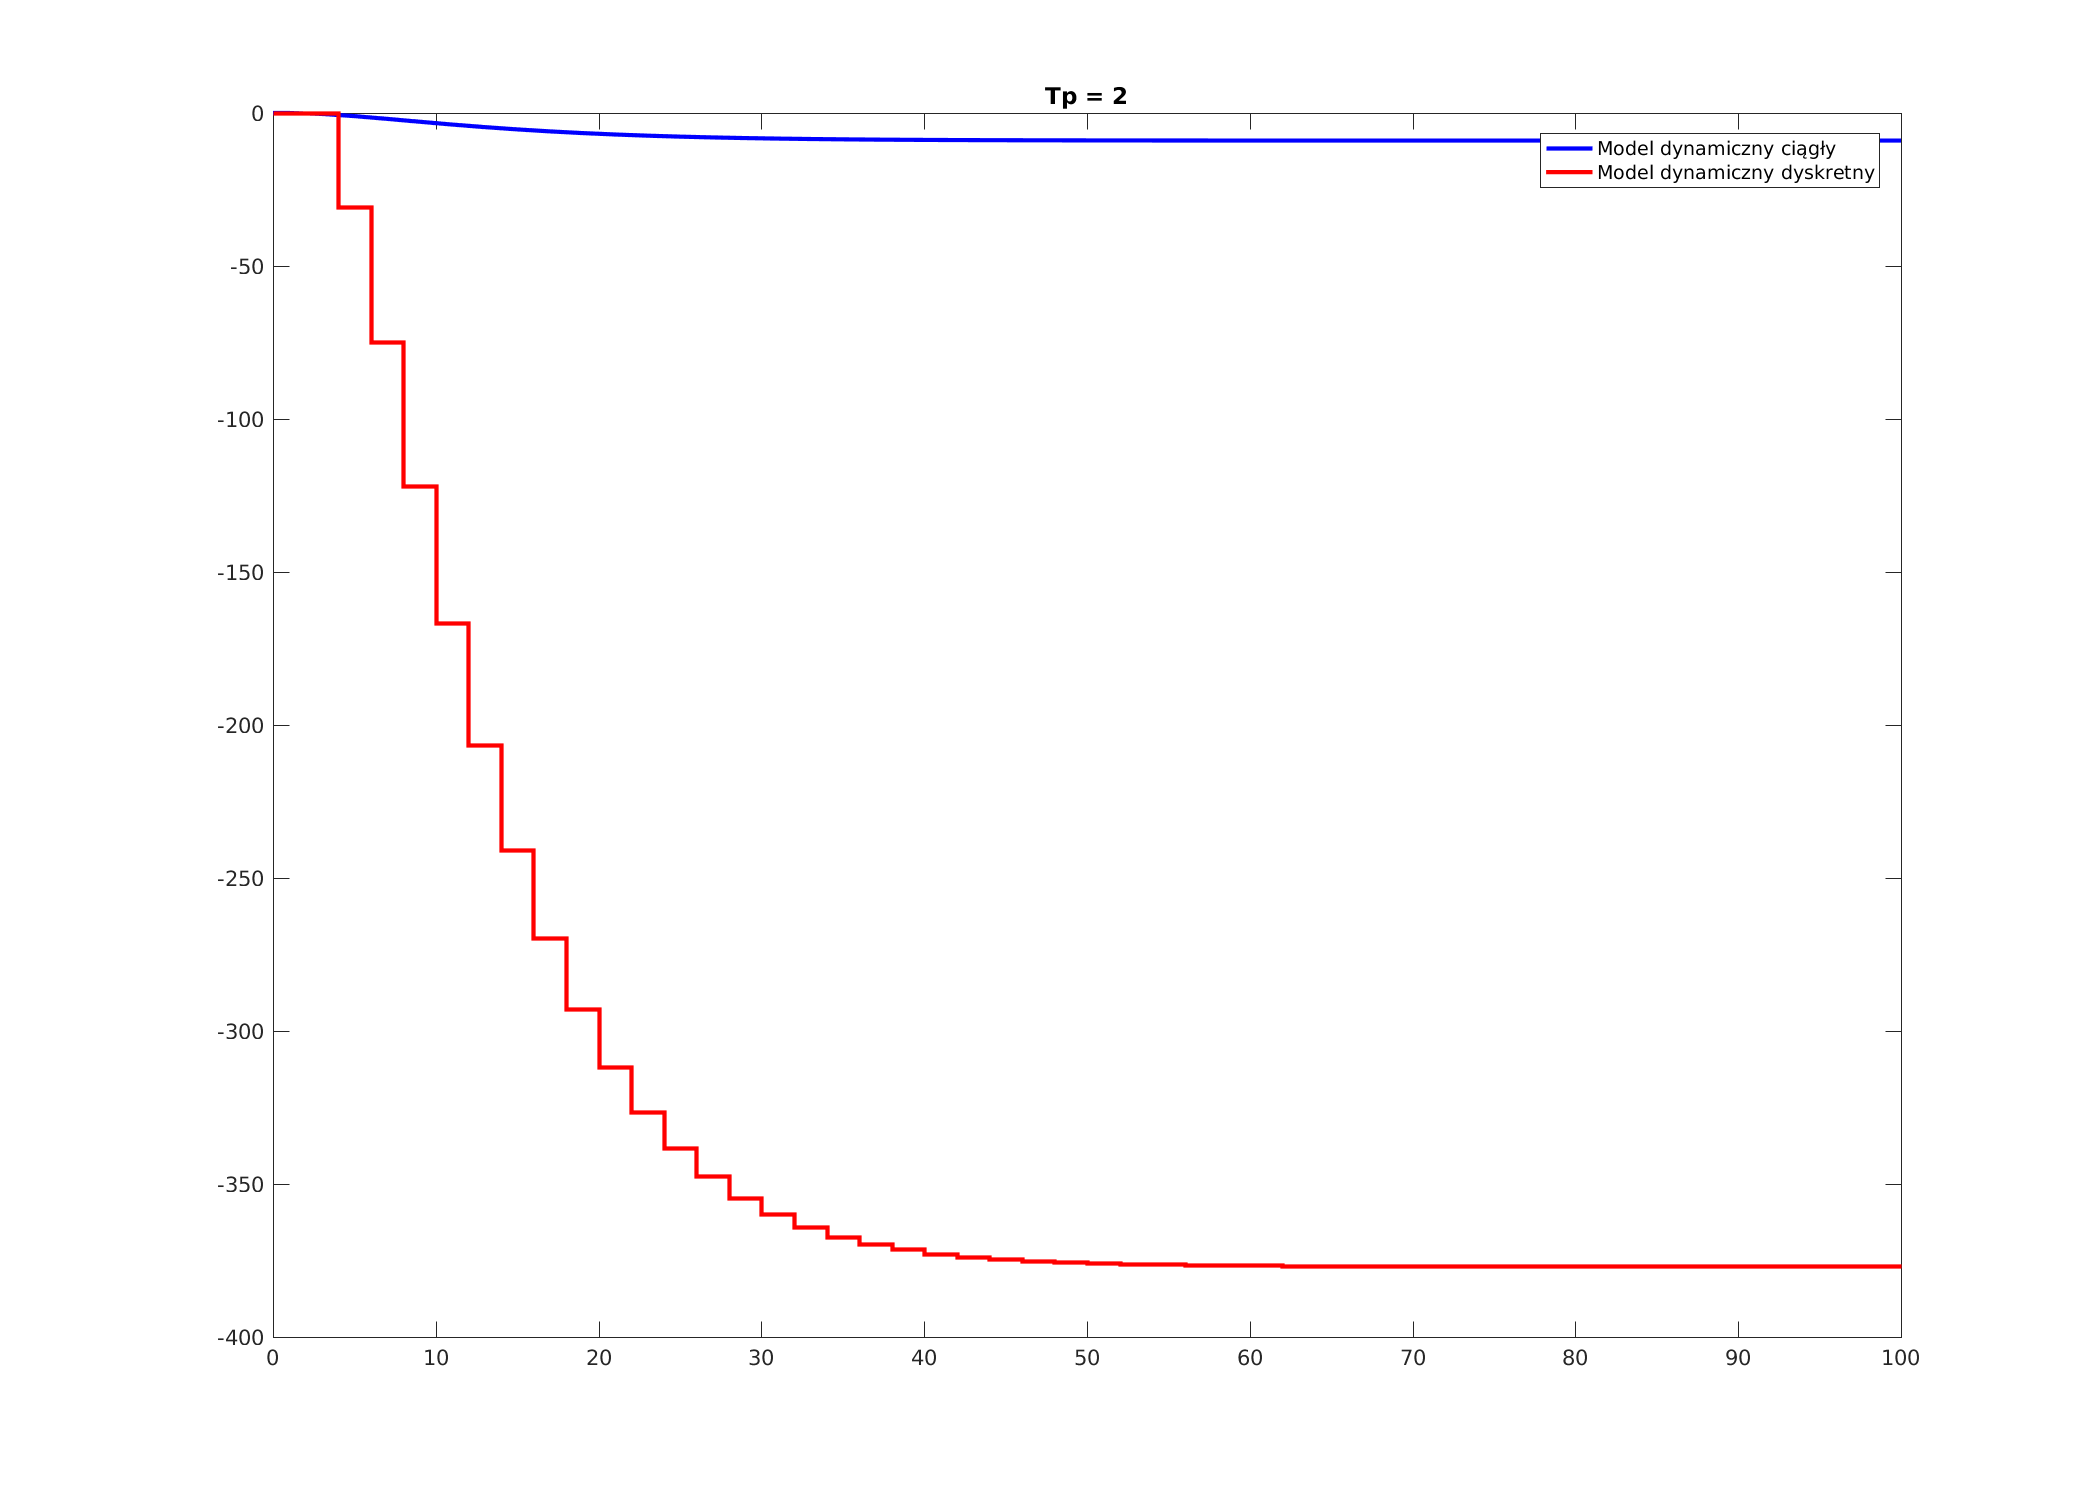
\includegraphics[scale=0.45]{tp_2.png}
\end{figure}
 
\section{Charakterystyka statyczna modelu ciągłego}
\subsection{Wyprowadzenie}


$\indent0 = -\frac{1}{T_{1}T_{2}}x_1 + \frac{K}{T_{1}T_{2}}(\alpha_1u + \alpha_2u^2 + \alpha_3u^3 + \alpha_4u^4)$
\\

$\frac{1}{T_{1}T_{2}}x_1 =  \frac{K}{T_{1}T_{2}}(\alpha_1u + \alpha_2u^2 + \alpha_3u^3 + \alpha_4u^4)/\cdot T_1T_2$
\\

$y = x_1 = K(\alpha_1u + \alpha_2u^2 + \alpha_3u^3 + \alpha_4u^4)$\\

Gdzie : \\

$K  = 5.5,\alpha_1 = 0.19, \alpha_2 = -0.05, \alpha_3 = -0.95, \alpha_4 = -0.45$
\subsection{Wykres}
\begin{figure}[H]
\centering
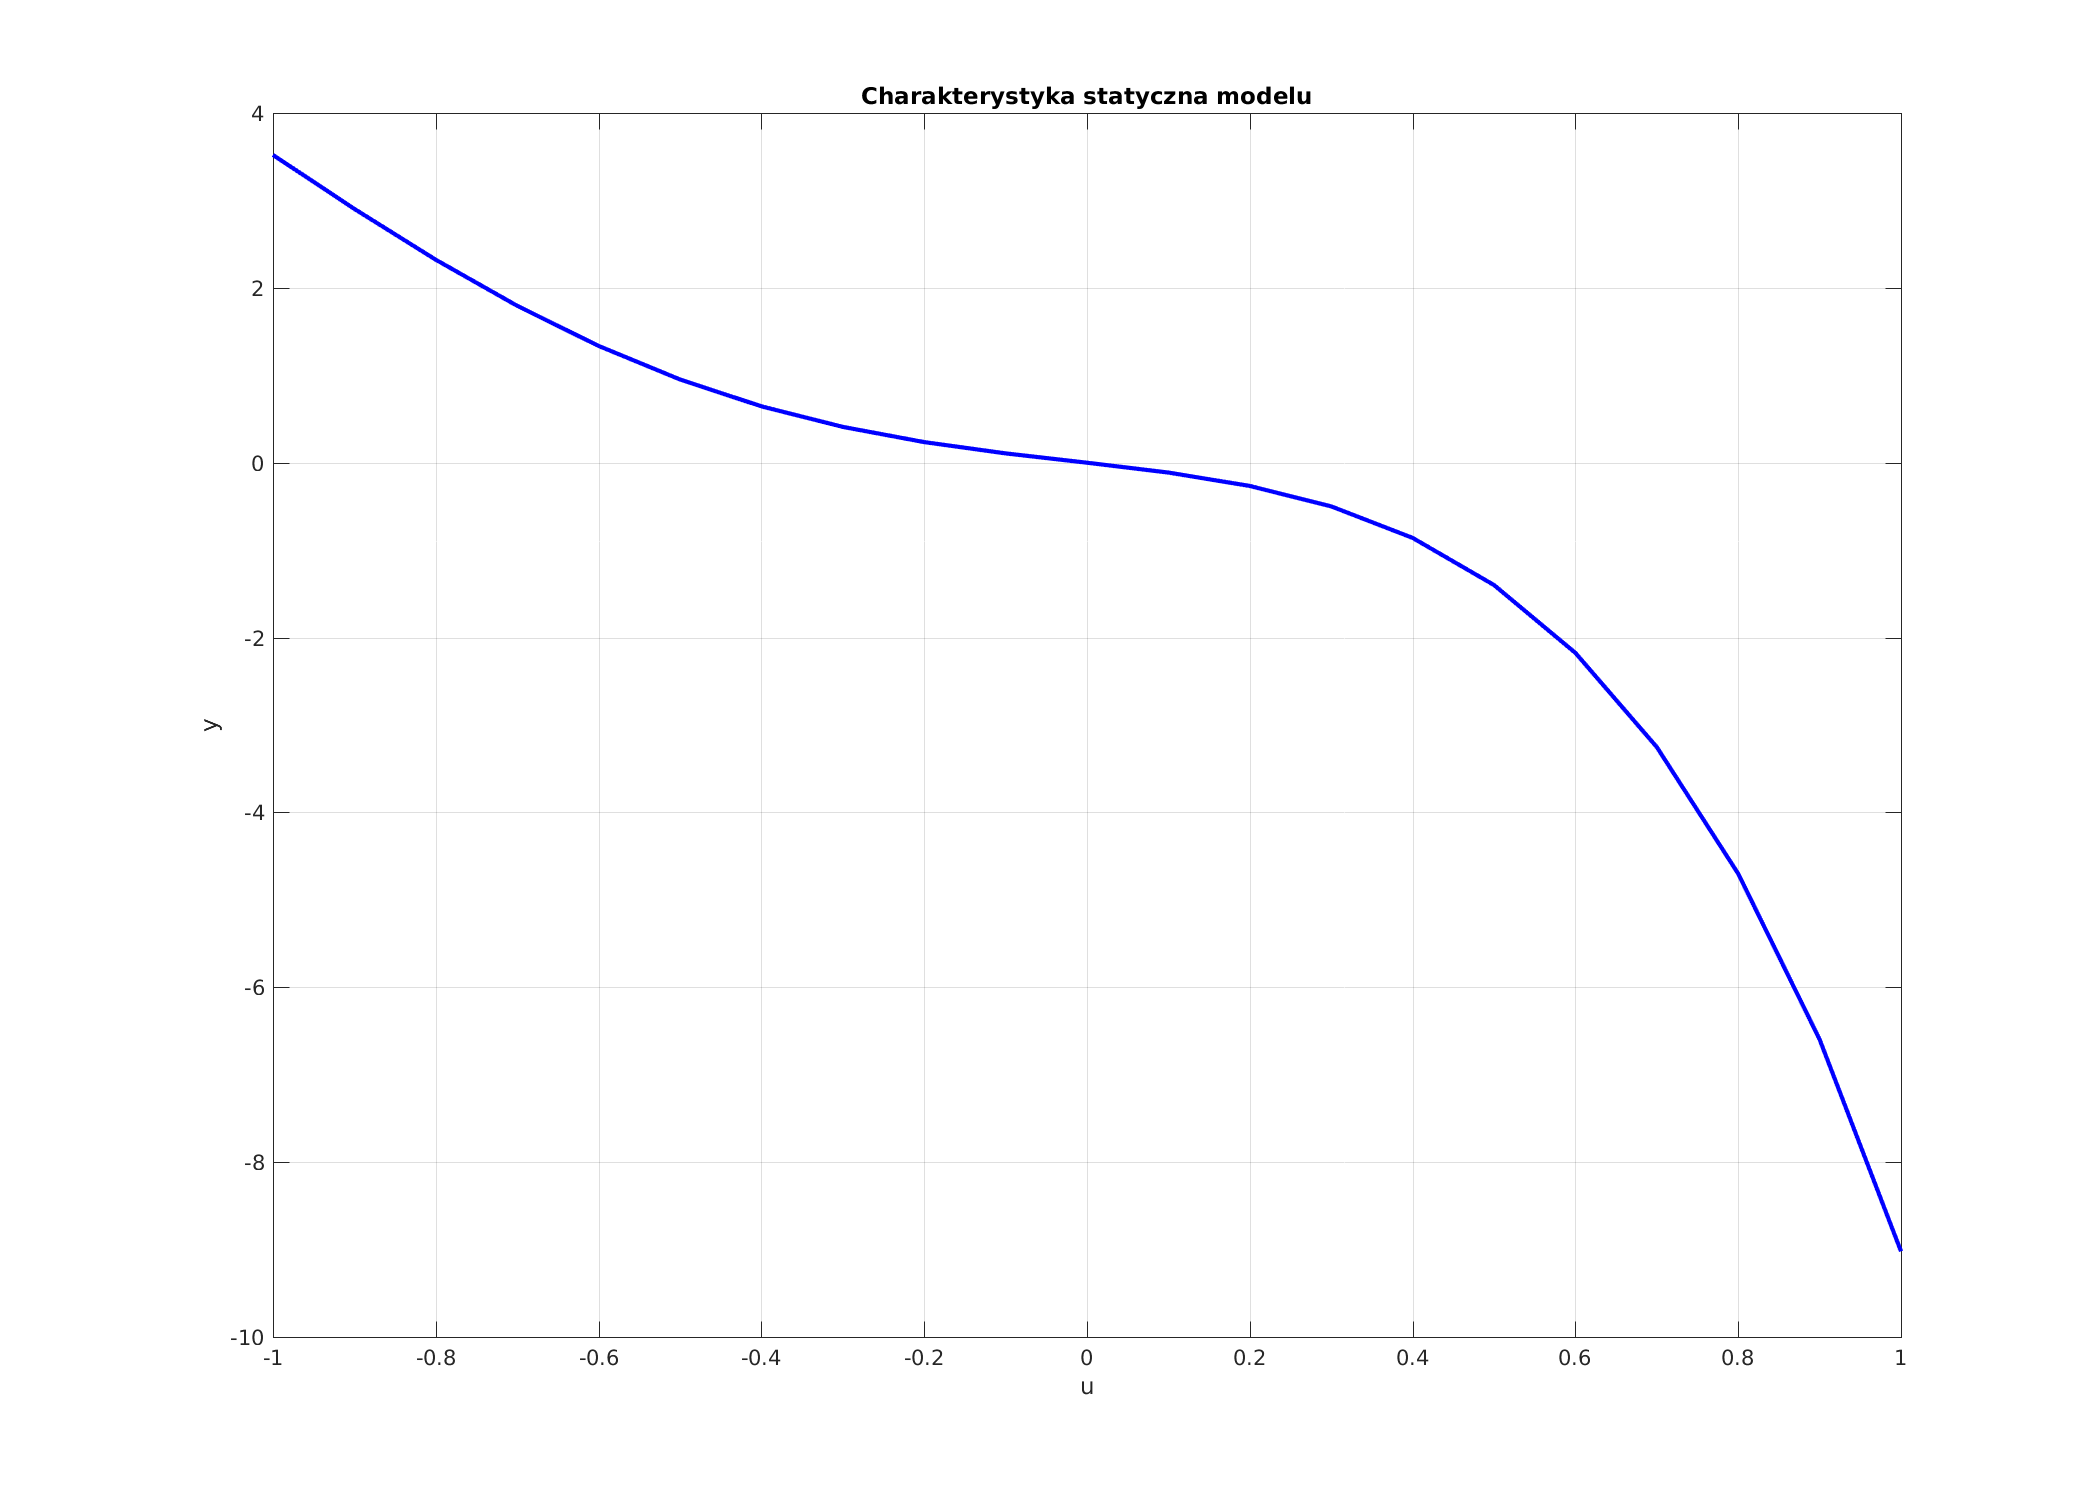
\includegraphics[scale=0.5]{statyczna.png}
\caption{Wykres charakterystyki statycznej modelu ciągłego}
\end{figure}


\section{Charakterystyka statyczna zlinearyzowana}

$\indent \overline{u}$ - punkt linearyzacji 
\\

$y_{stat} = K(\alpha_1\overline{u} + \alpha_2\overline{u}^2 + \alpha_3\overline{u}^3 + \alpha_4\overline{u}^4)
+ K(\alpha_1 + \alpha_22\overline{u} + \alpha_33\overline{u}^2 + \alpha_44\overline{u}^3)(u-\overline{u})$
\\

$y_{stat} = K(\alpha_1u + \alpha_2(2\overline{u}u - \overline{u}^2)+ \alpha_3(3\overline{u}^2u-2\overline{u}^3) + \alpha_4(4\overline{u}^3u - 3\overline{u}^4))$

\section{Wykresy zlinearyzowanej charakterystyki statycznej}
\begin{figure}[H]
\centering
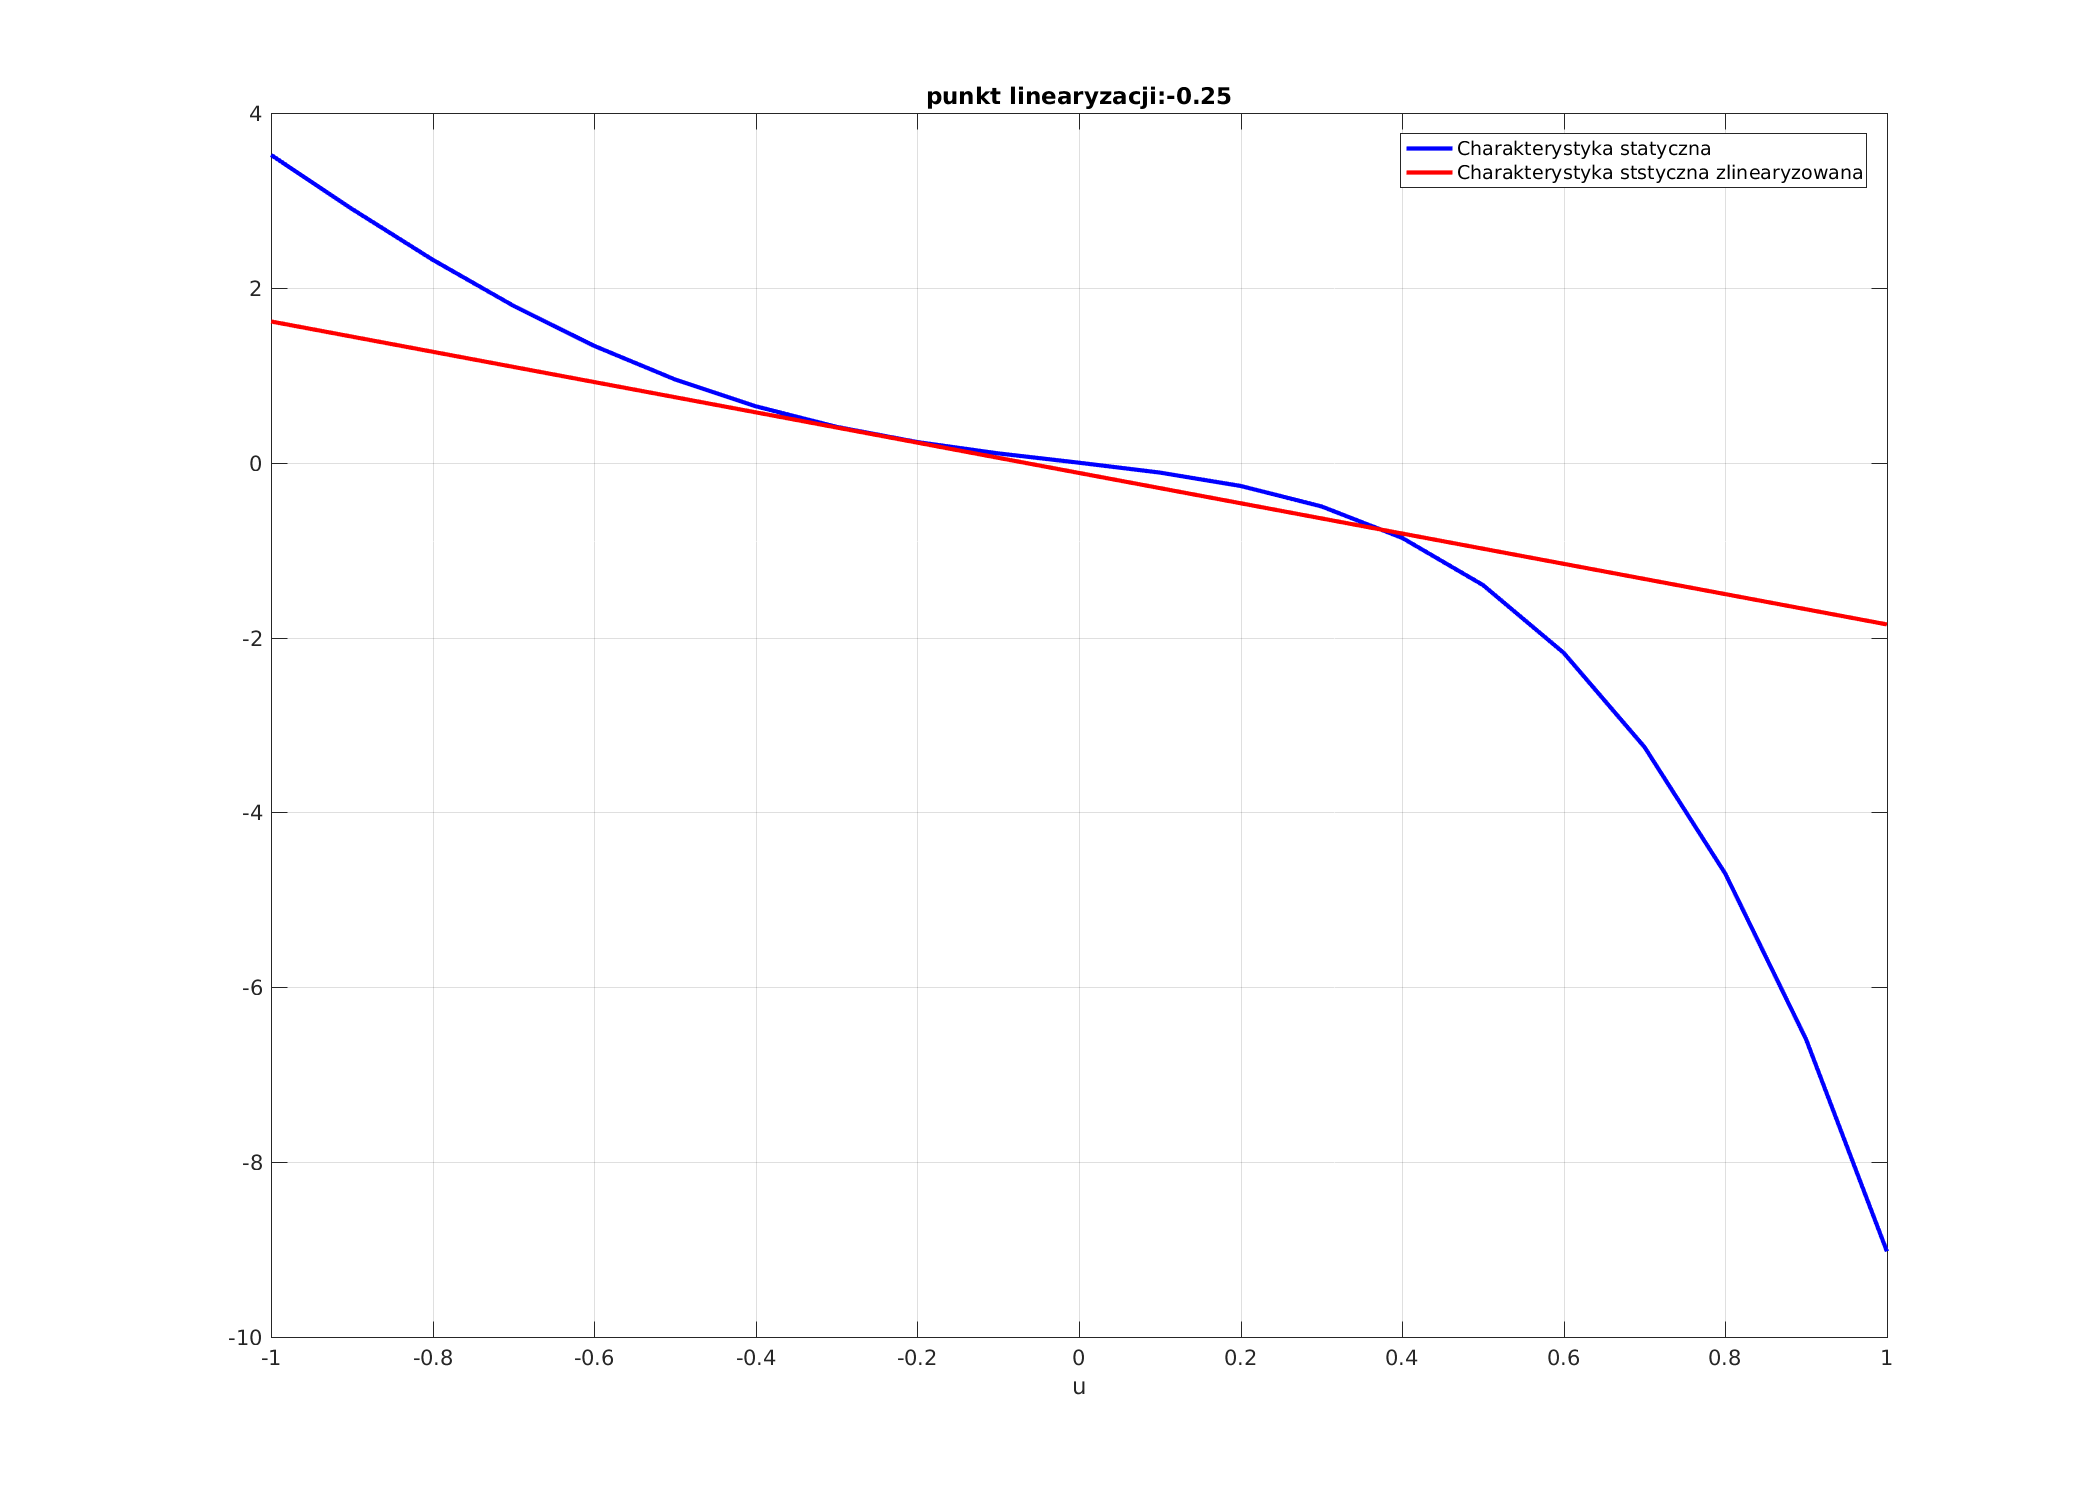
\includegraphics[scale=0.45]{6_-0,25.png}
\end{figure}
\begin{figure}[H]
\centering
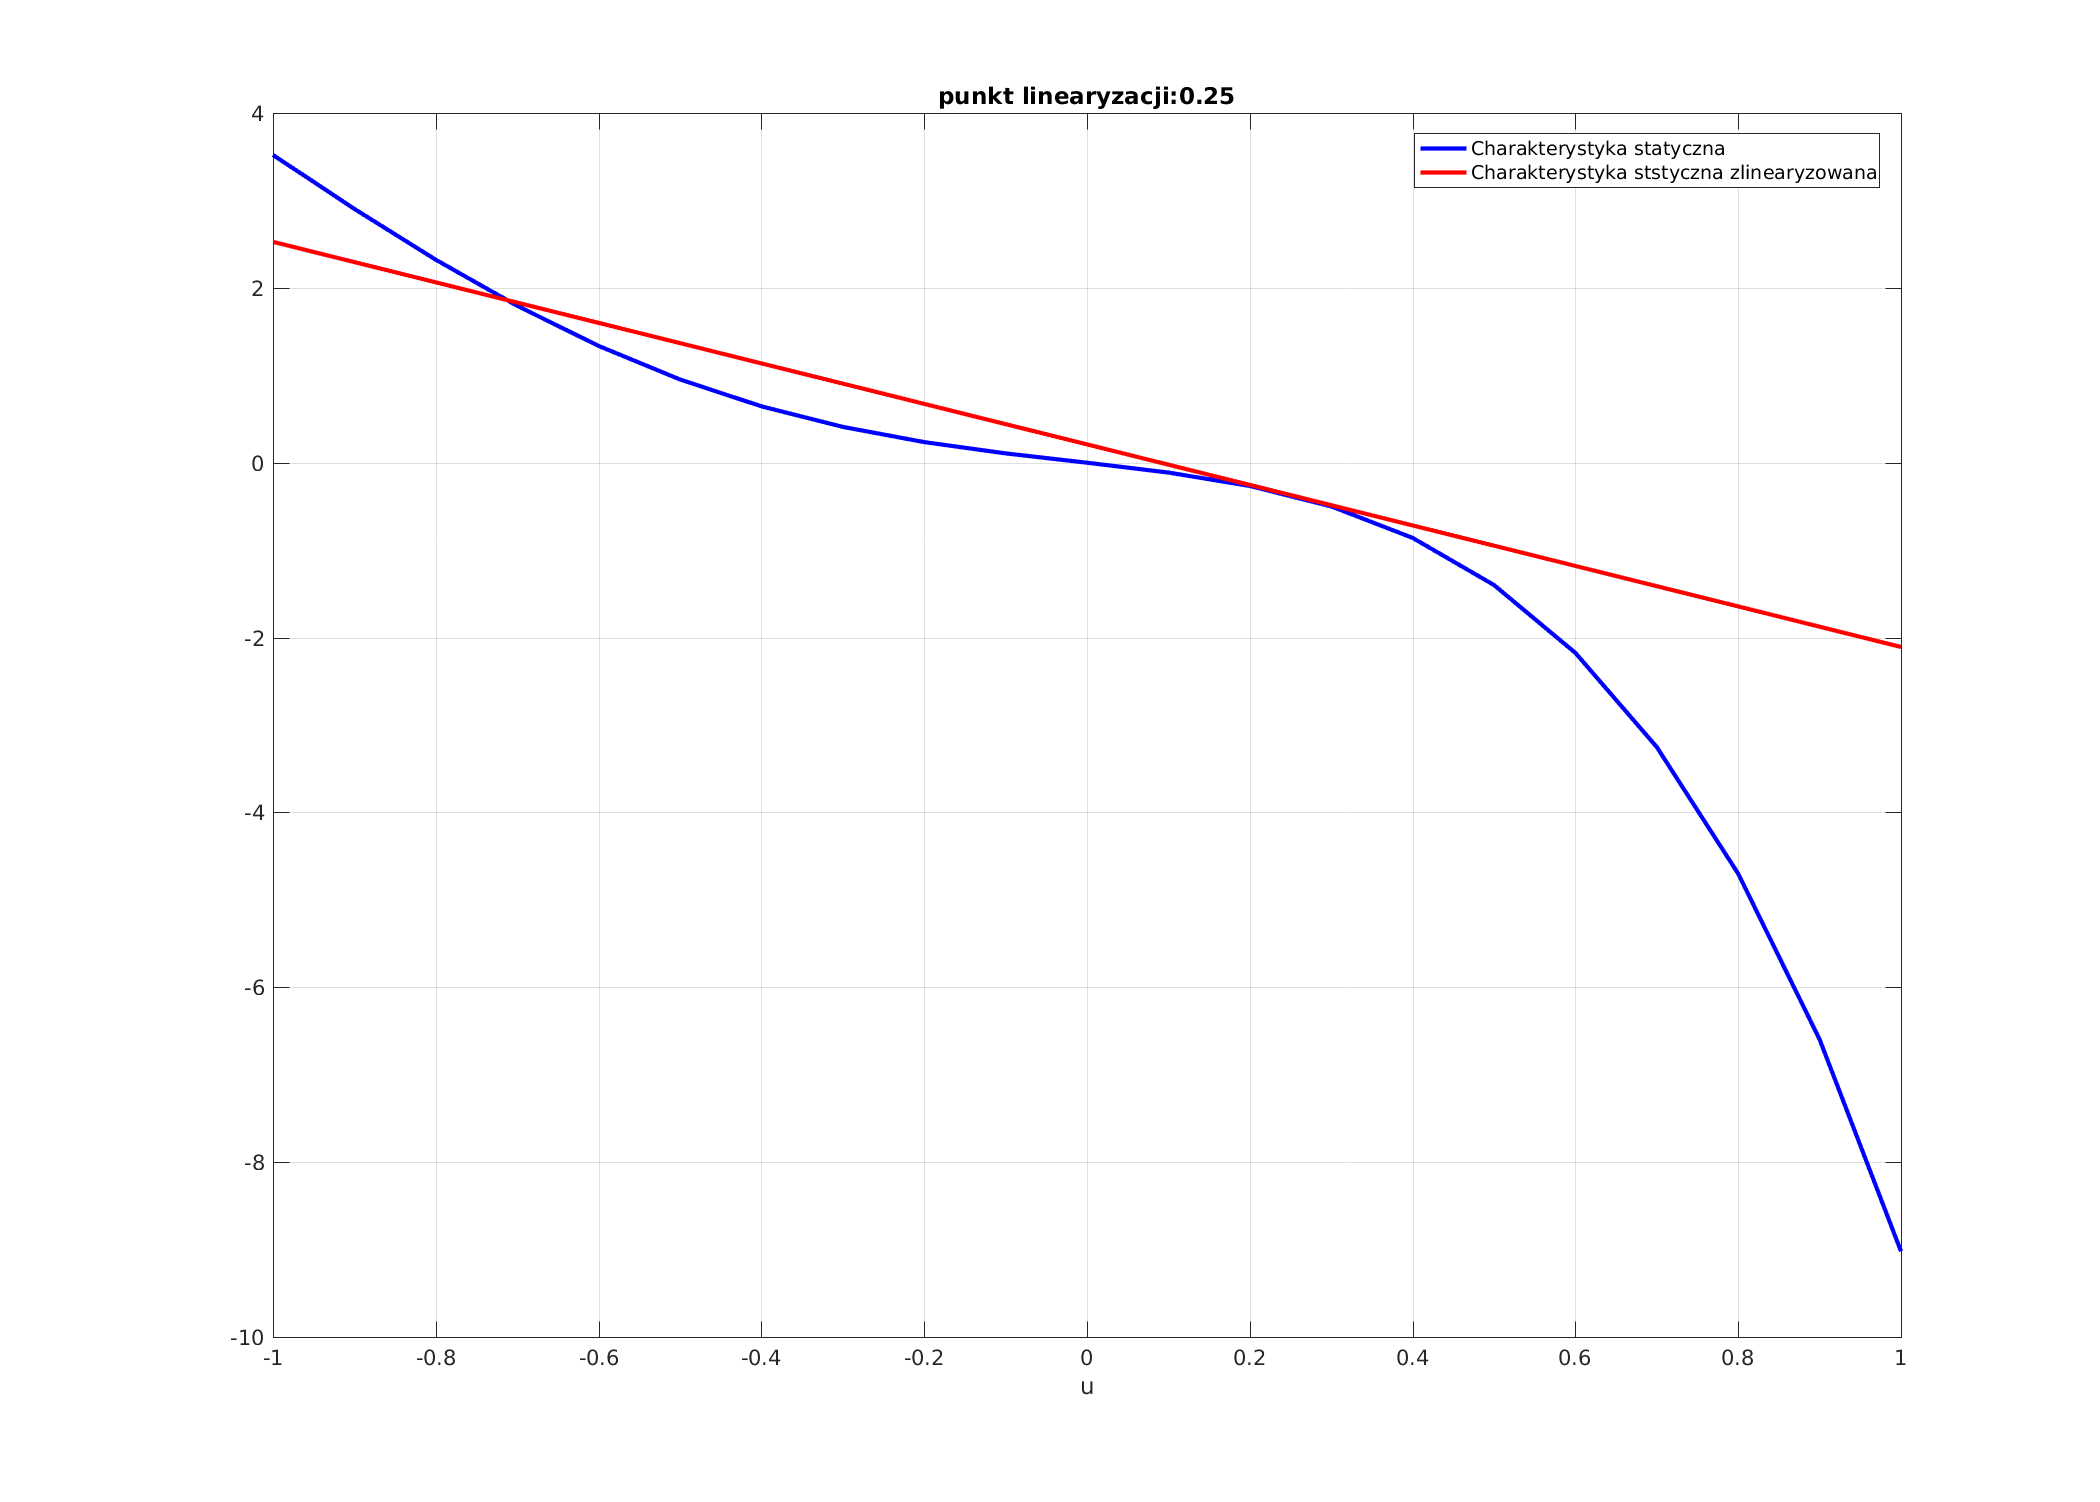
\includegraphics[scale=0.45]{6_0,25.png}
\end{figure}
\begin{figure}[H]
\centering
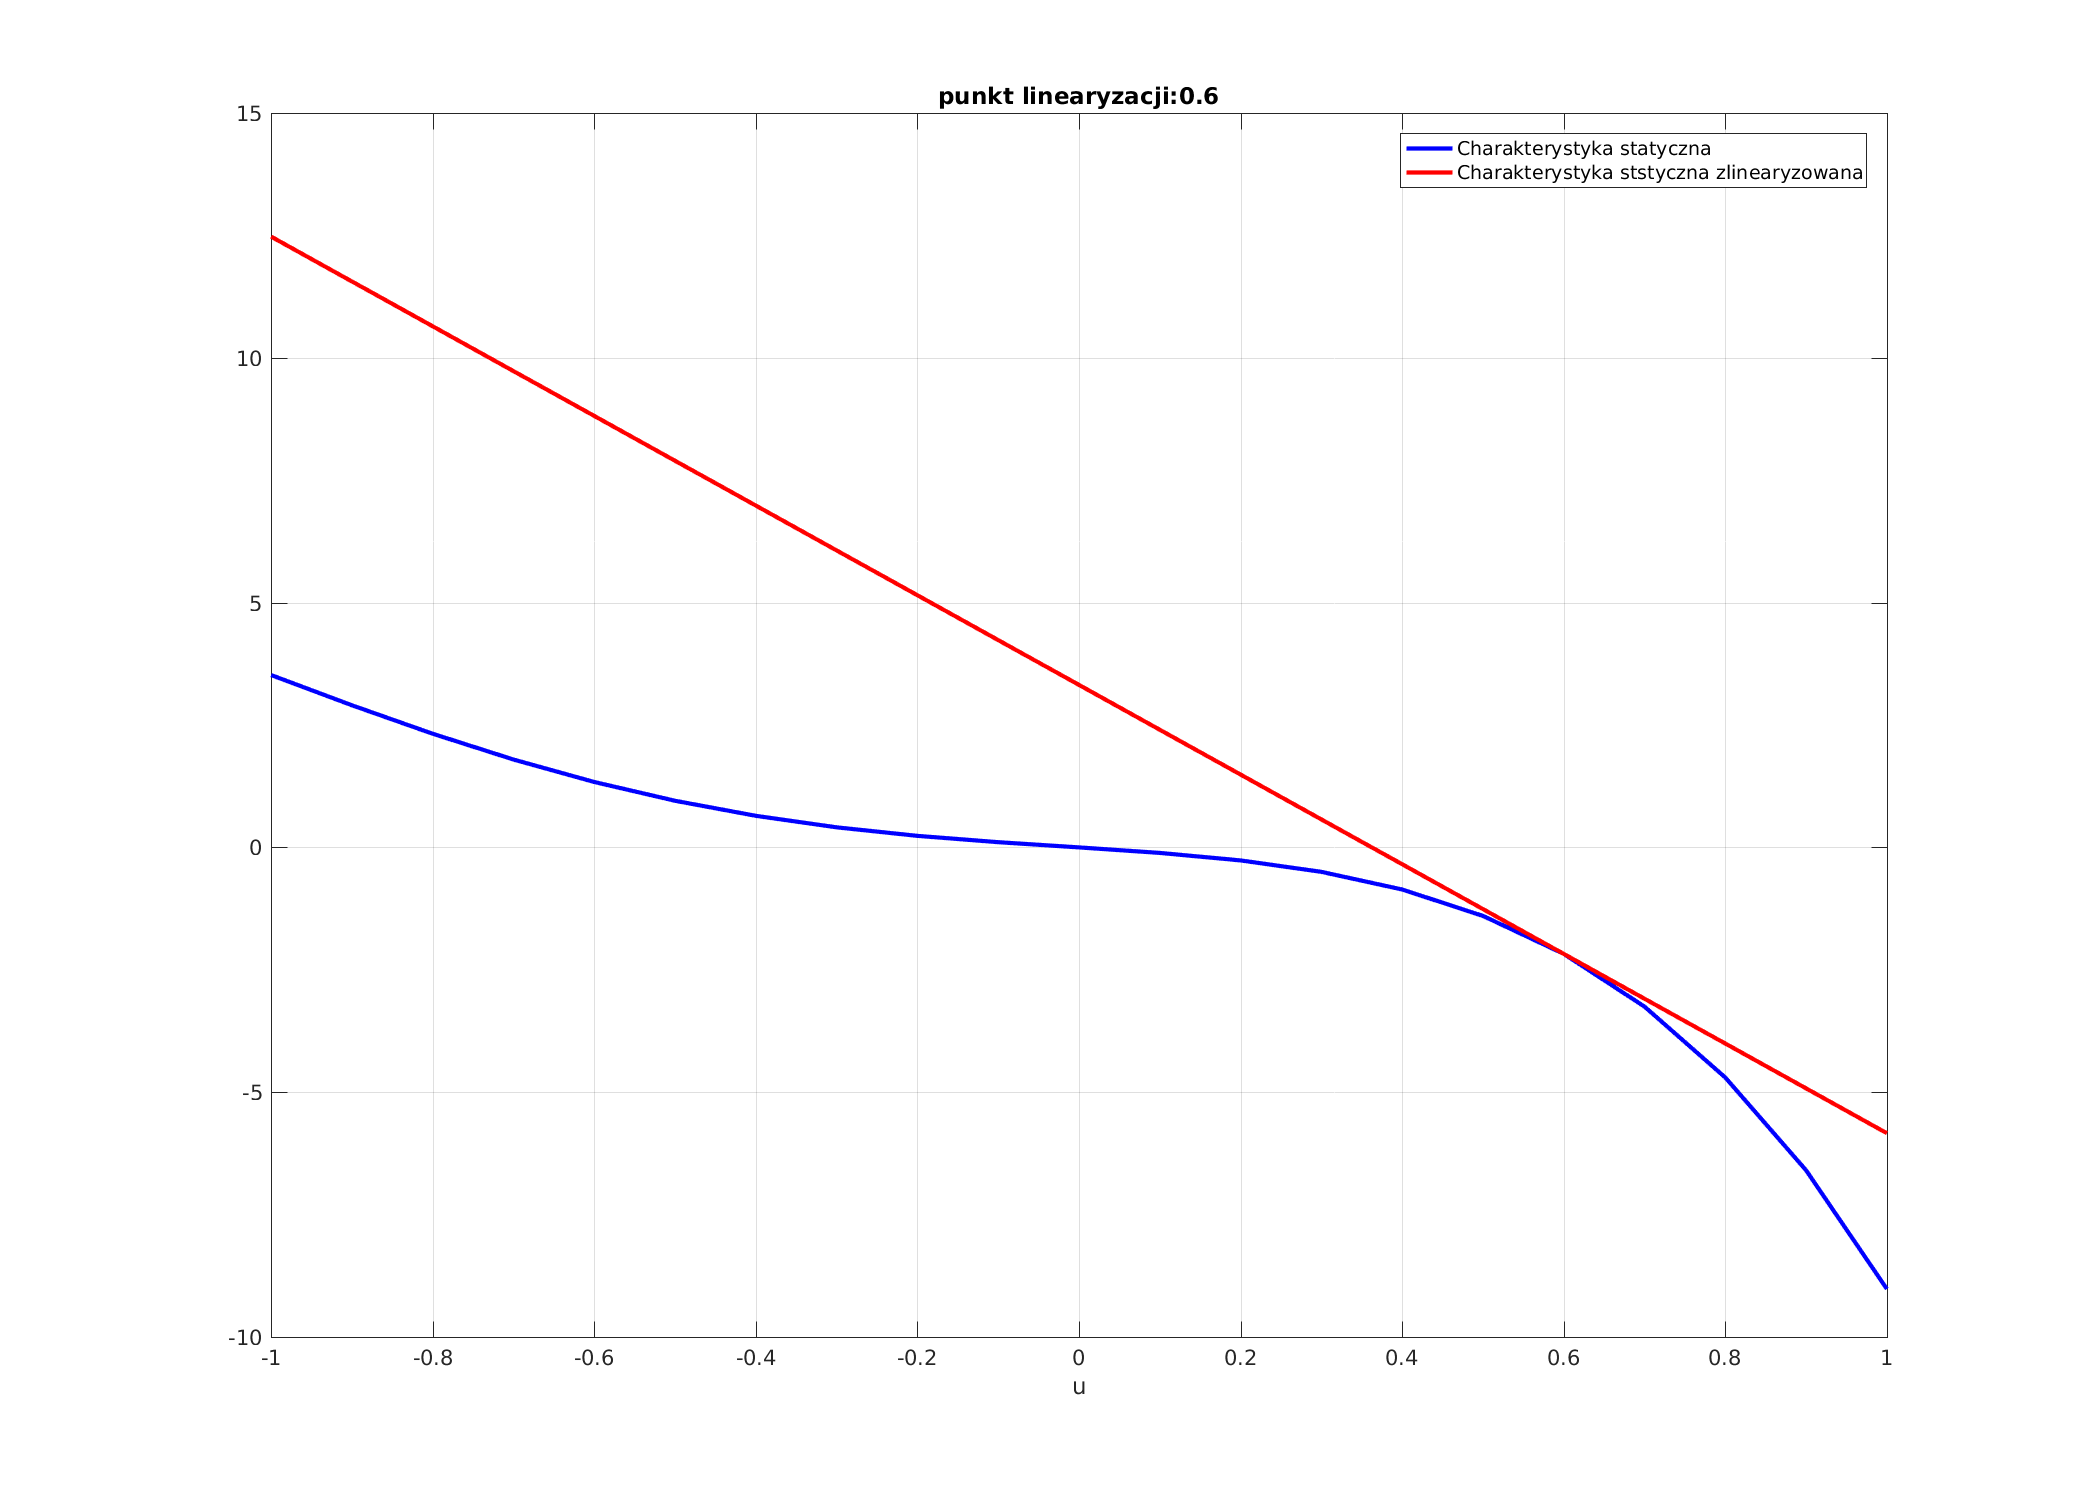
\includegraphics[scale=0.45]{6_0,6.png}
\end{figure}
\begin{figure}[H]
\centering
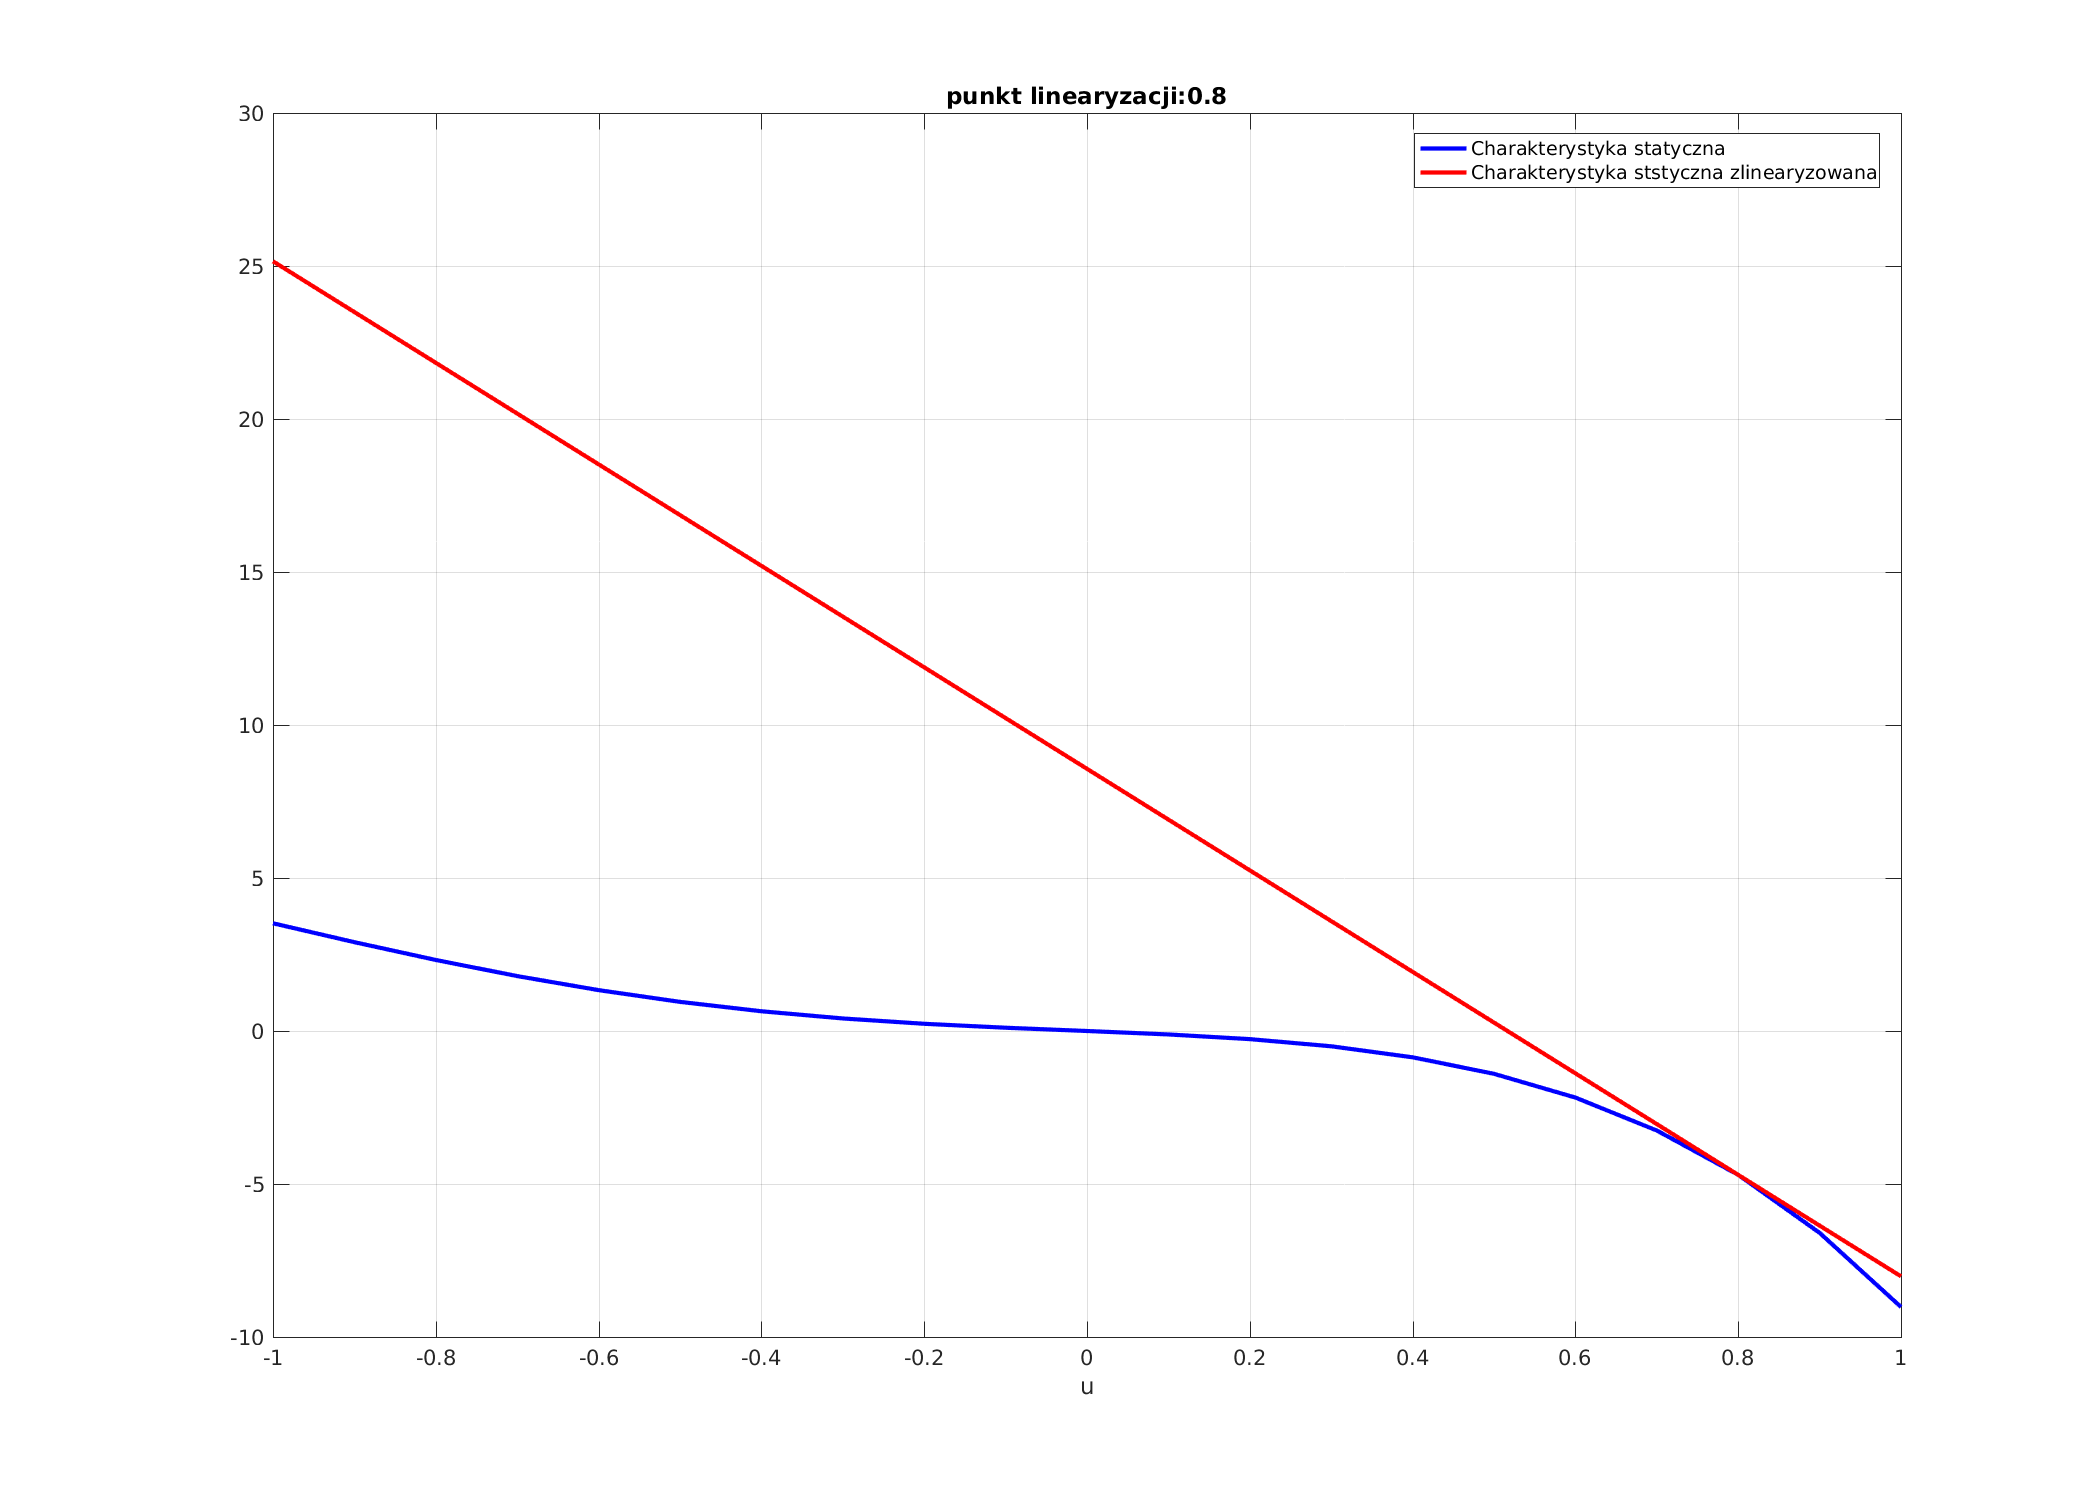
\includegraphics[scale=0.45]{6_0,8.png}
\end{figure}

\section{Dynamiczny dyskretny model zlinearyzowany}
Dynamiczny model dyskretny opisany jest równianiami:
\\

$x_1(k) =(1-\frac{(T_1 + T_2)T_p}{T_1T_2})x_1(k-1)+T_px_2(k-1) $
\\

$x_2(k) = - \frac{T_p}{T_1T_2}x_1(k-1) + x_2(k-1) + T_p(\alpha_1u(k-1)+\alpha_2u^2(k-1)\\
	\indent	+ \alpha_3u^3(k-1)+\alpha_4u^4(k-1))$
\\

$y(k) = x_1(k)$
\\
\\

\noindent Aby otrzymać model liniowy należy zlinearyzować wszystkie nieliniowe elementy równań stanu:
\\

$\overline{u}$ - punkt linearyzacji 
\\

$\alpha_2u^2(k-1)+ \alpha_3u^3(k-1)+\alpha_4u^4(k-1) \approx \alpha_2\overline{u}^2 + \alpha_3\overline{u}^3 + \alpha_4\overline{u}^4 + (\alpha_22\overline{u} + \alpha_33\overline{u}^2 + \alpha_44\overline{u}^3)(u-\overline{u})  \\ \indent \approx \alpha_2(2\overline{u}u - \overline{u}^2)+ \alpha_3(3\overline{u}^2u-2\overline{u}^3) + \alpha_4(4\overline{u}^3u - 3\overline{u}^4)$
\\

\noindent po podstawieniu do równania modelu otrzymujemy: 
\\

$x_1(k) =(1-\frac{(T_1 + T_2)T_p}{T_1T_2})x_1(k-1)+T_px_2(k-1) $
\\

$x_2(k) = - \frac{T_p}{T_1T_2}x_1(k-1) + x_2(k-1) + T_p(\alpha_1u(k-1)+\alpha_2(2\overline{u}u(k-1) - \overline{u}^2)+
\\ \indent \alpha_3(3\overline{u}^2u(k-1)-2\overline{u}^3) + \alpha_4(4\overline{u}^3u(k-1) - 3\overline{u}^4))$
\\

$y(k) = x_1(k)$\\
\\
Gdzie : \\

$K  = 5.5, T_1 = 7, T_2 = 7, \alpha_1 = 0.19, \alpha_2 = -0.05, \alpha_3 = -0.95, \alpha_4 = -0.45, T_p$ - krok czasowy
\\

\section{Reprezentacja graficzna zlinearyzowanego dynamicznego modelu dyskretnego}\
\begin{figure}[H]
\centering
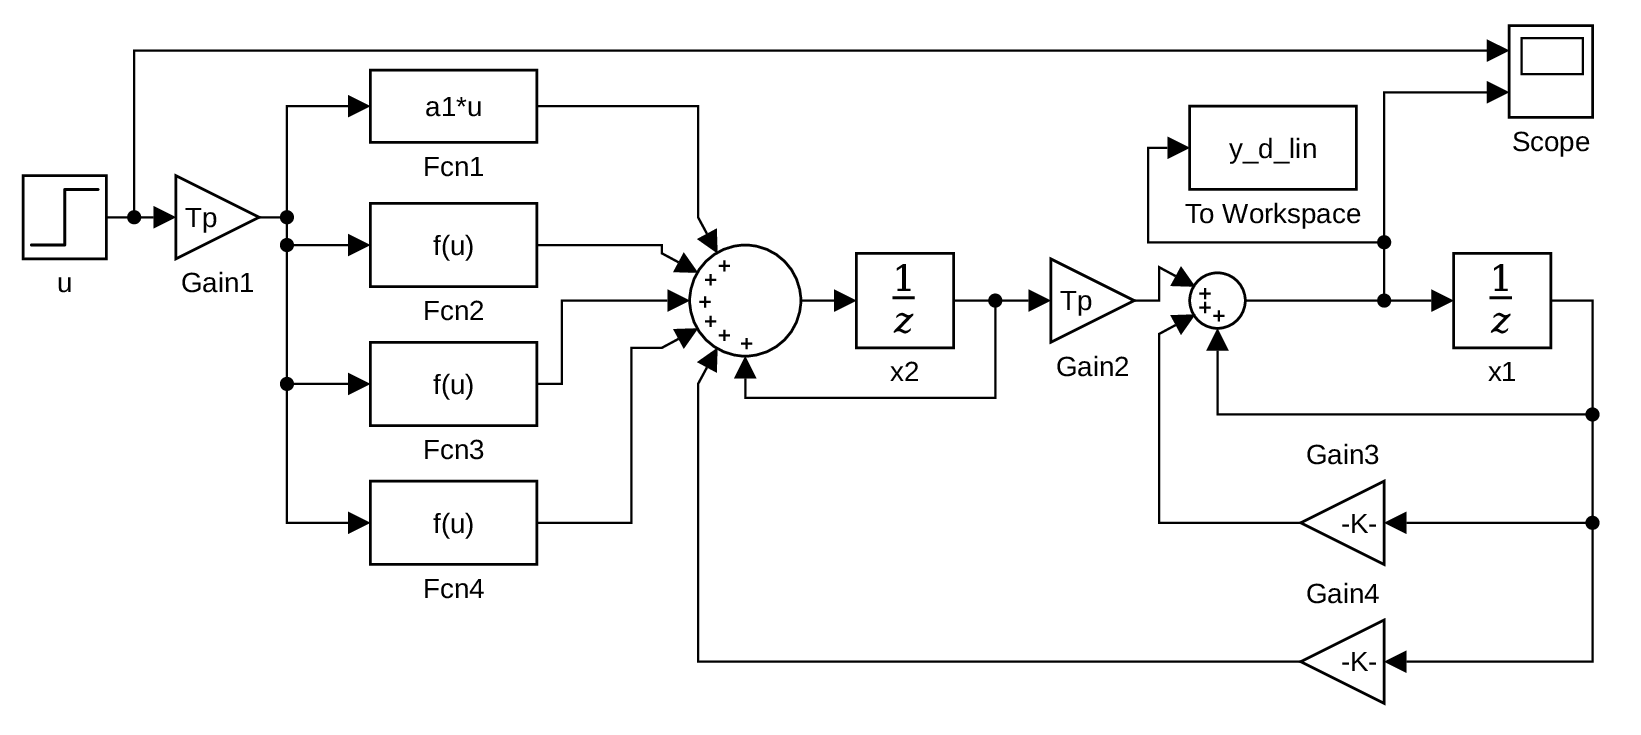
\includegraphics[scale=0.25]{dynamiczny_model_dyskretny_zlinearyzowany.png}
\caption{Reprezentacja graficzna dynamicznego modelu dyskretnego zlinearyzowanego }
\end{figure}

\section{Symulacja dynamicznego modelu dyskretnego}
\begin{figure}[H]
\centering
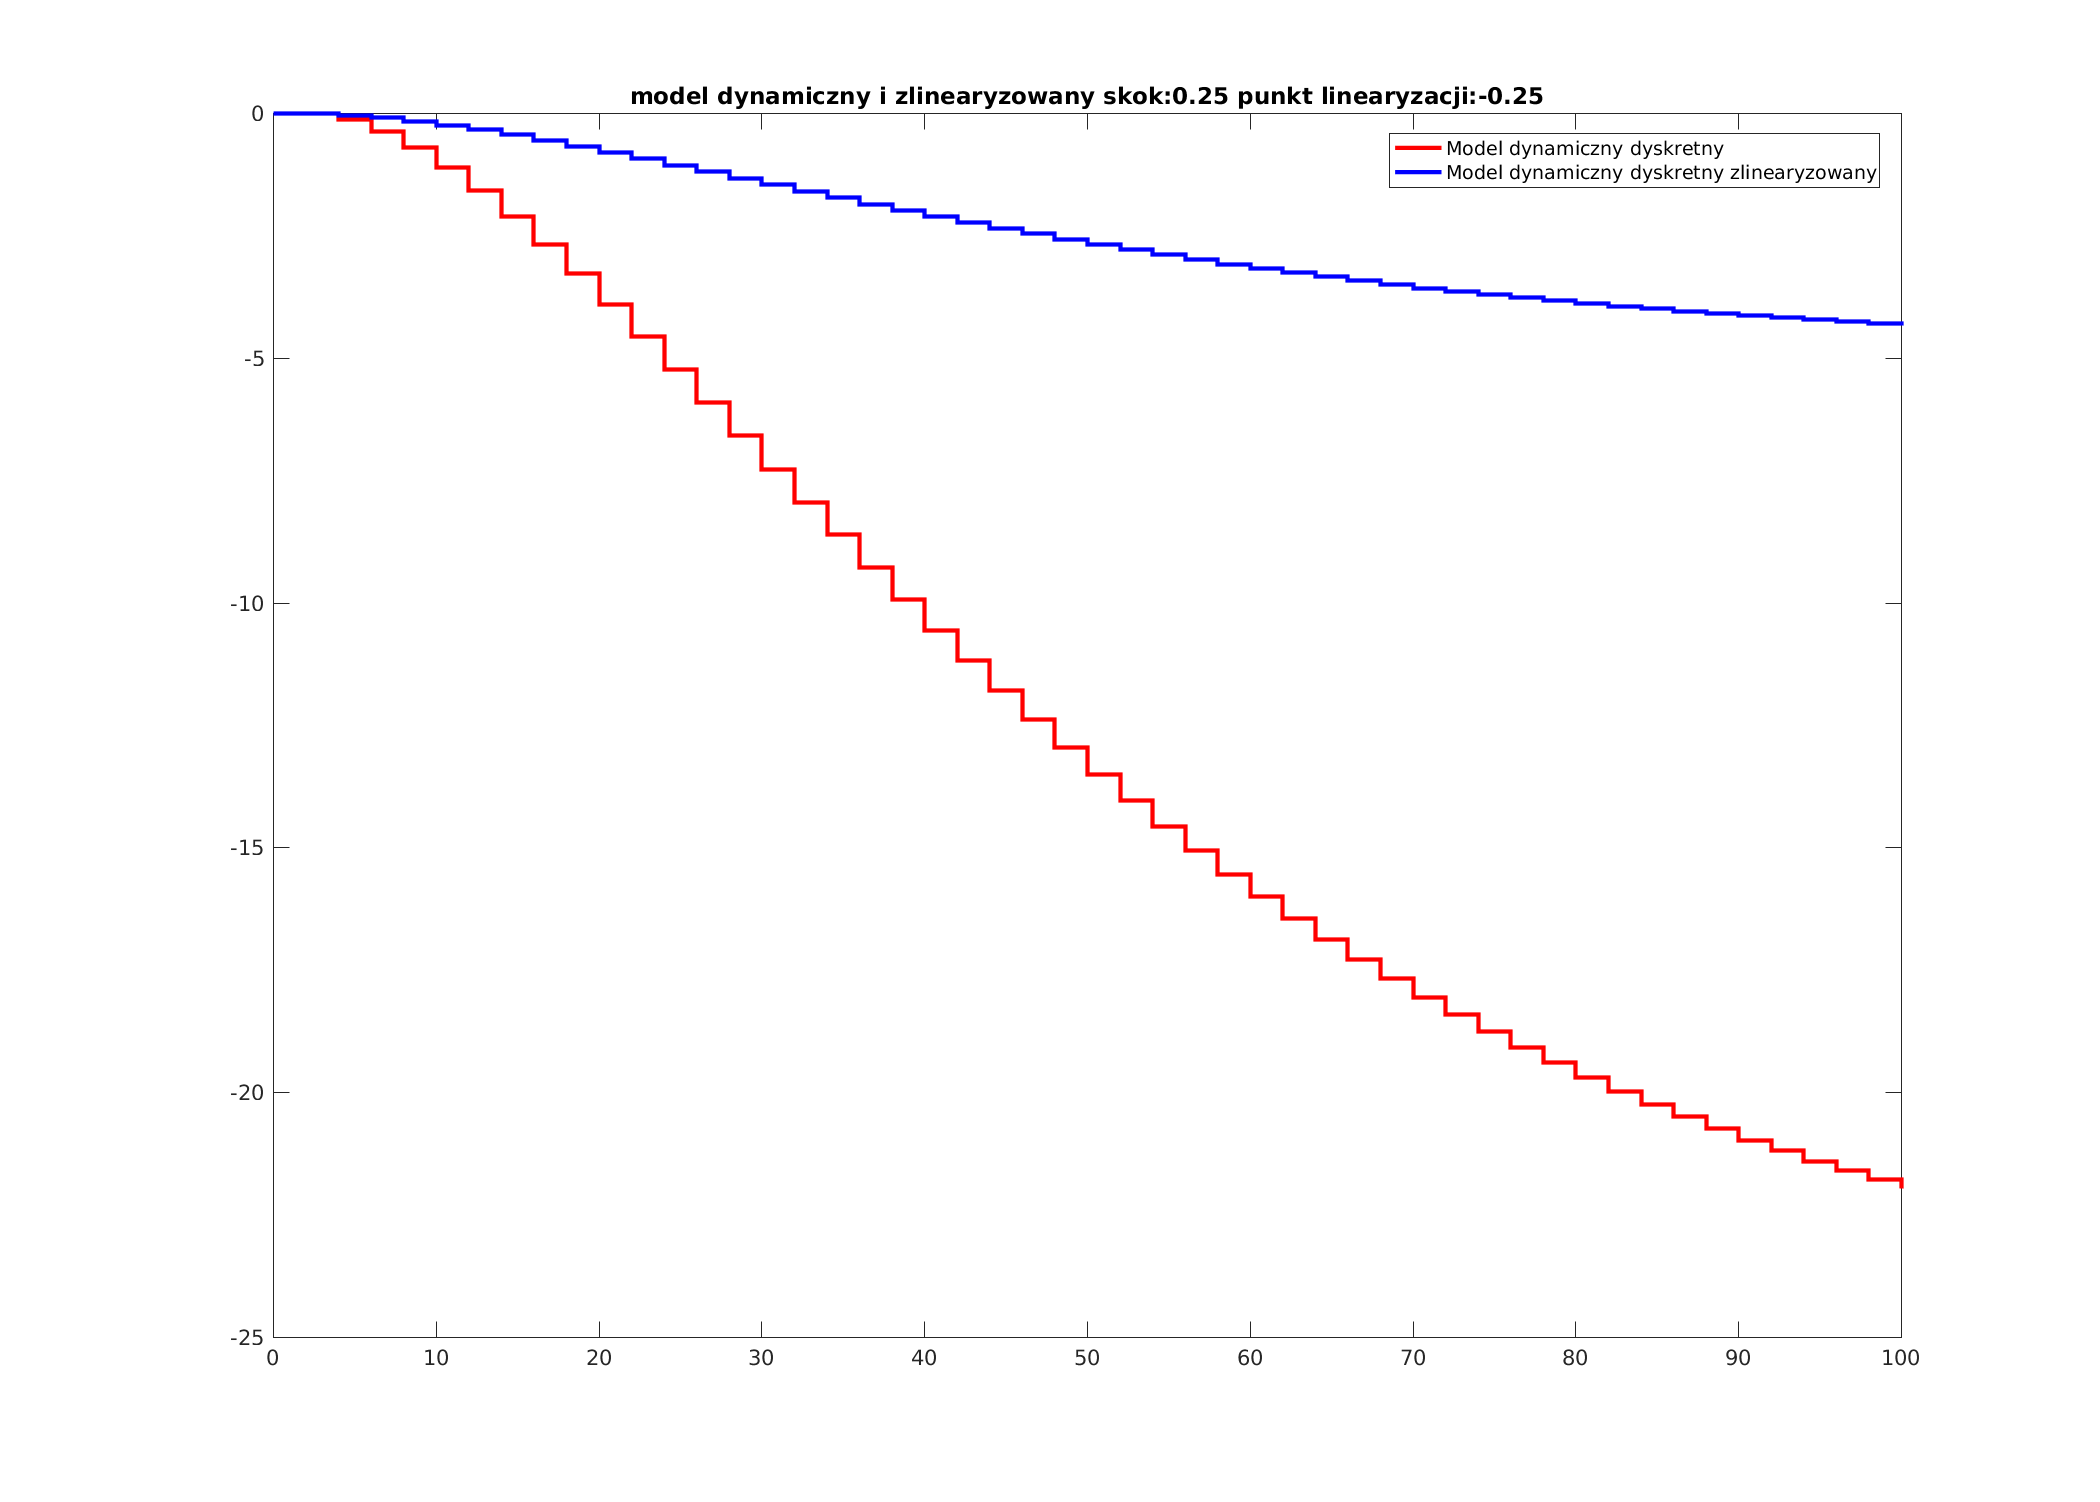
\includegraphics[scale=0.45]{925m25.png}
\end{figure}
\begin{figure}[H]
\centering
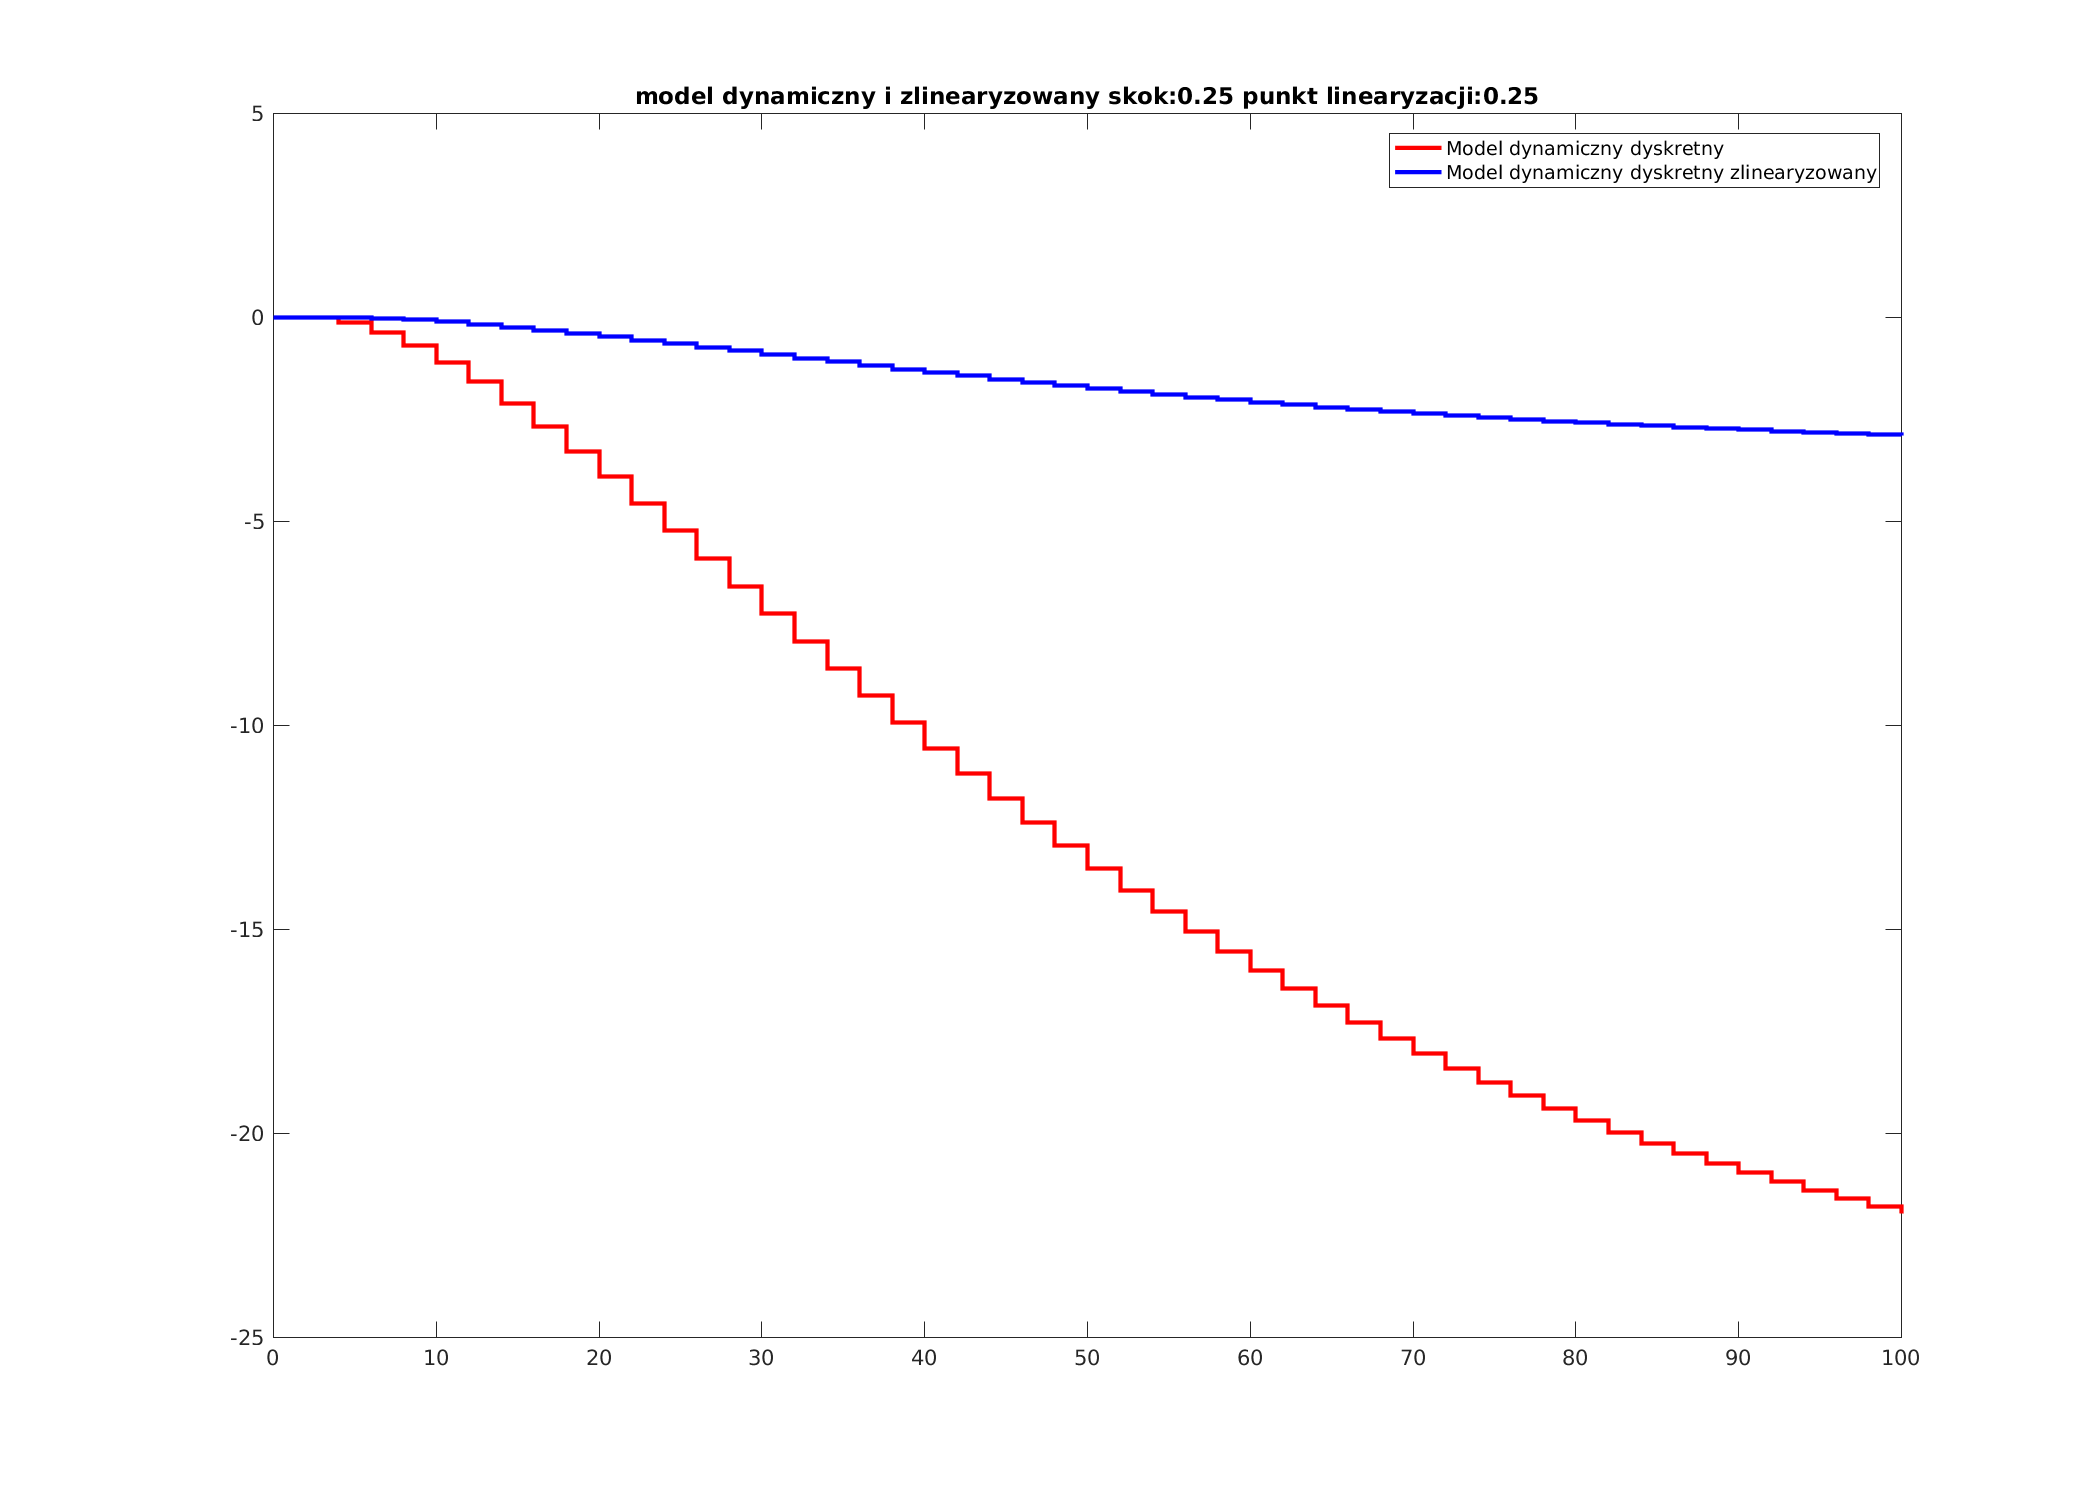
\includegraphics[scale=0.45]{92525.png}
\end{figure}
\begin{figure}[H]
\centering
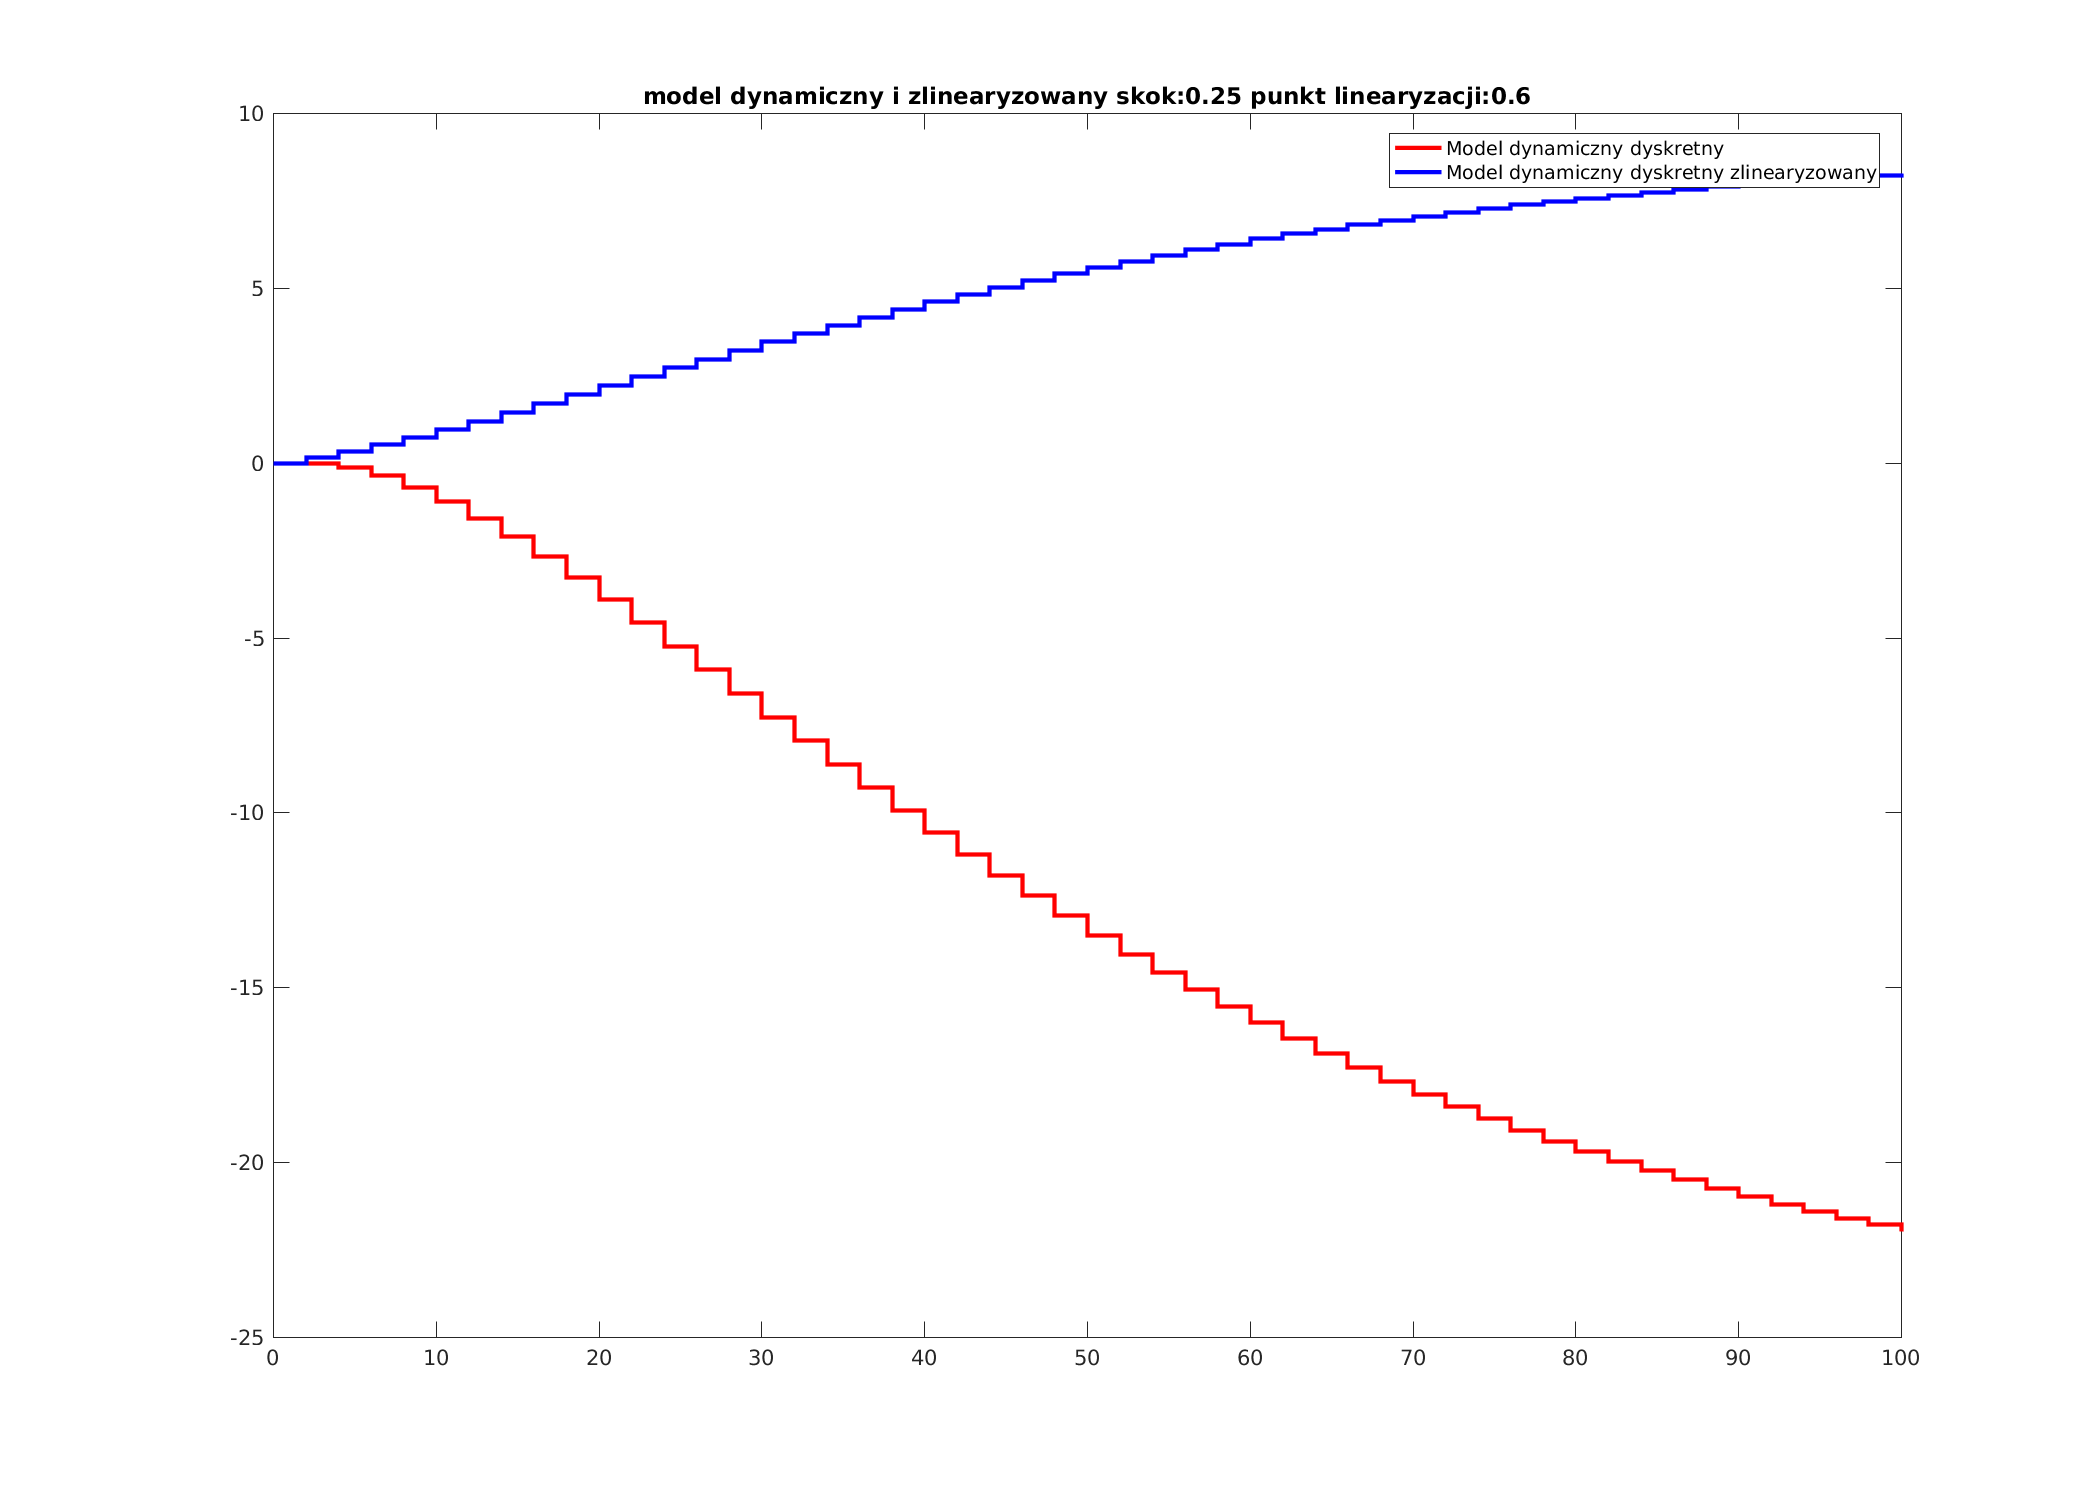
\includegraphics[scale=0.45]{9256.png}
\end{figure}
\begin{figure}[H]
\centering
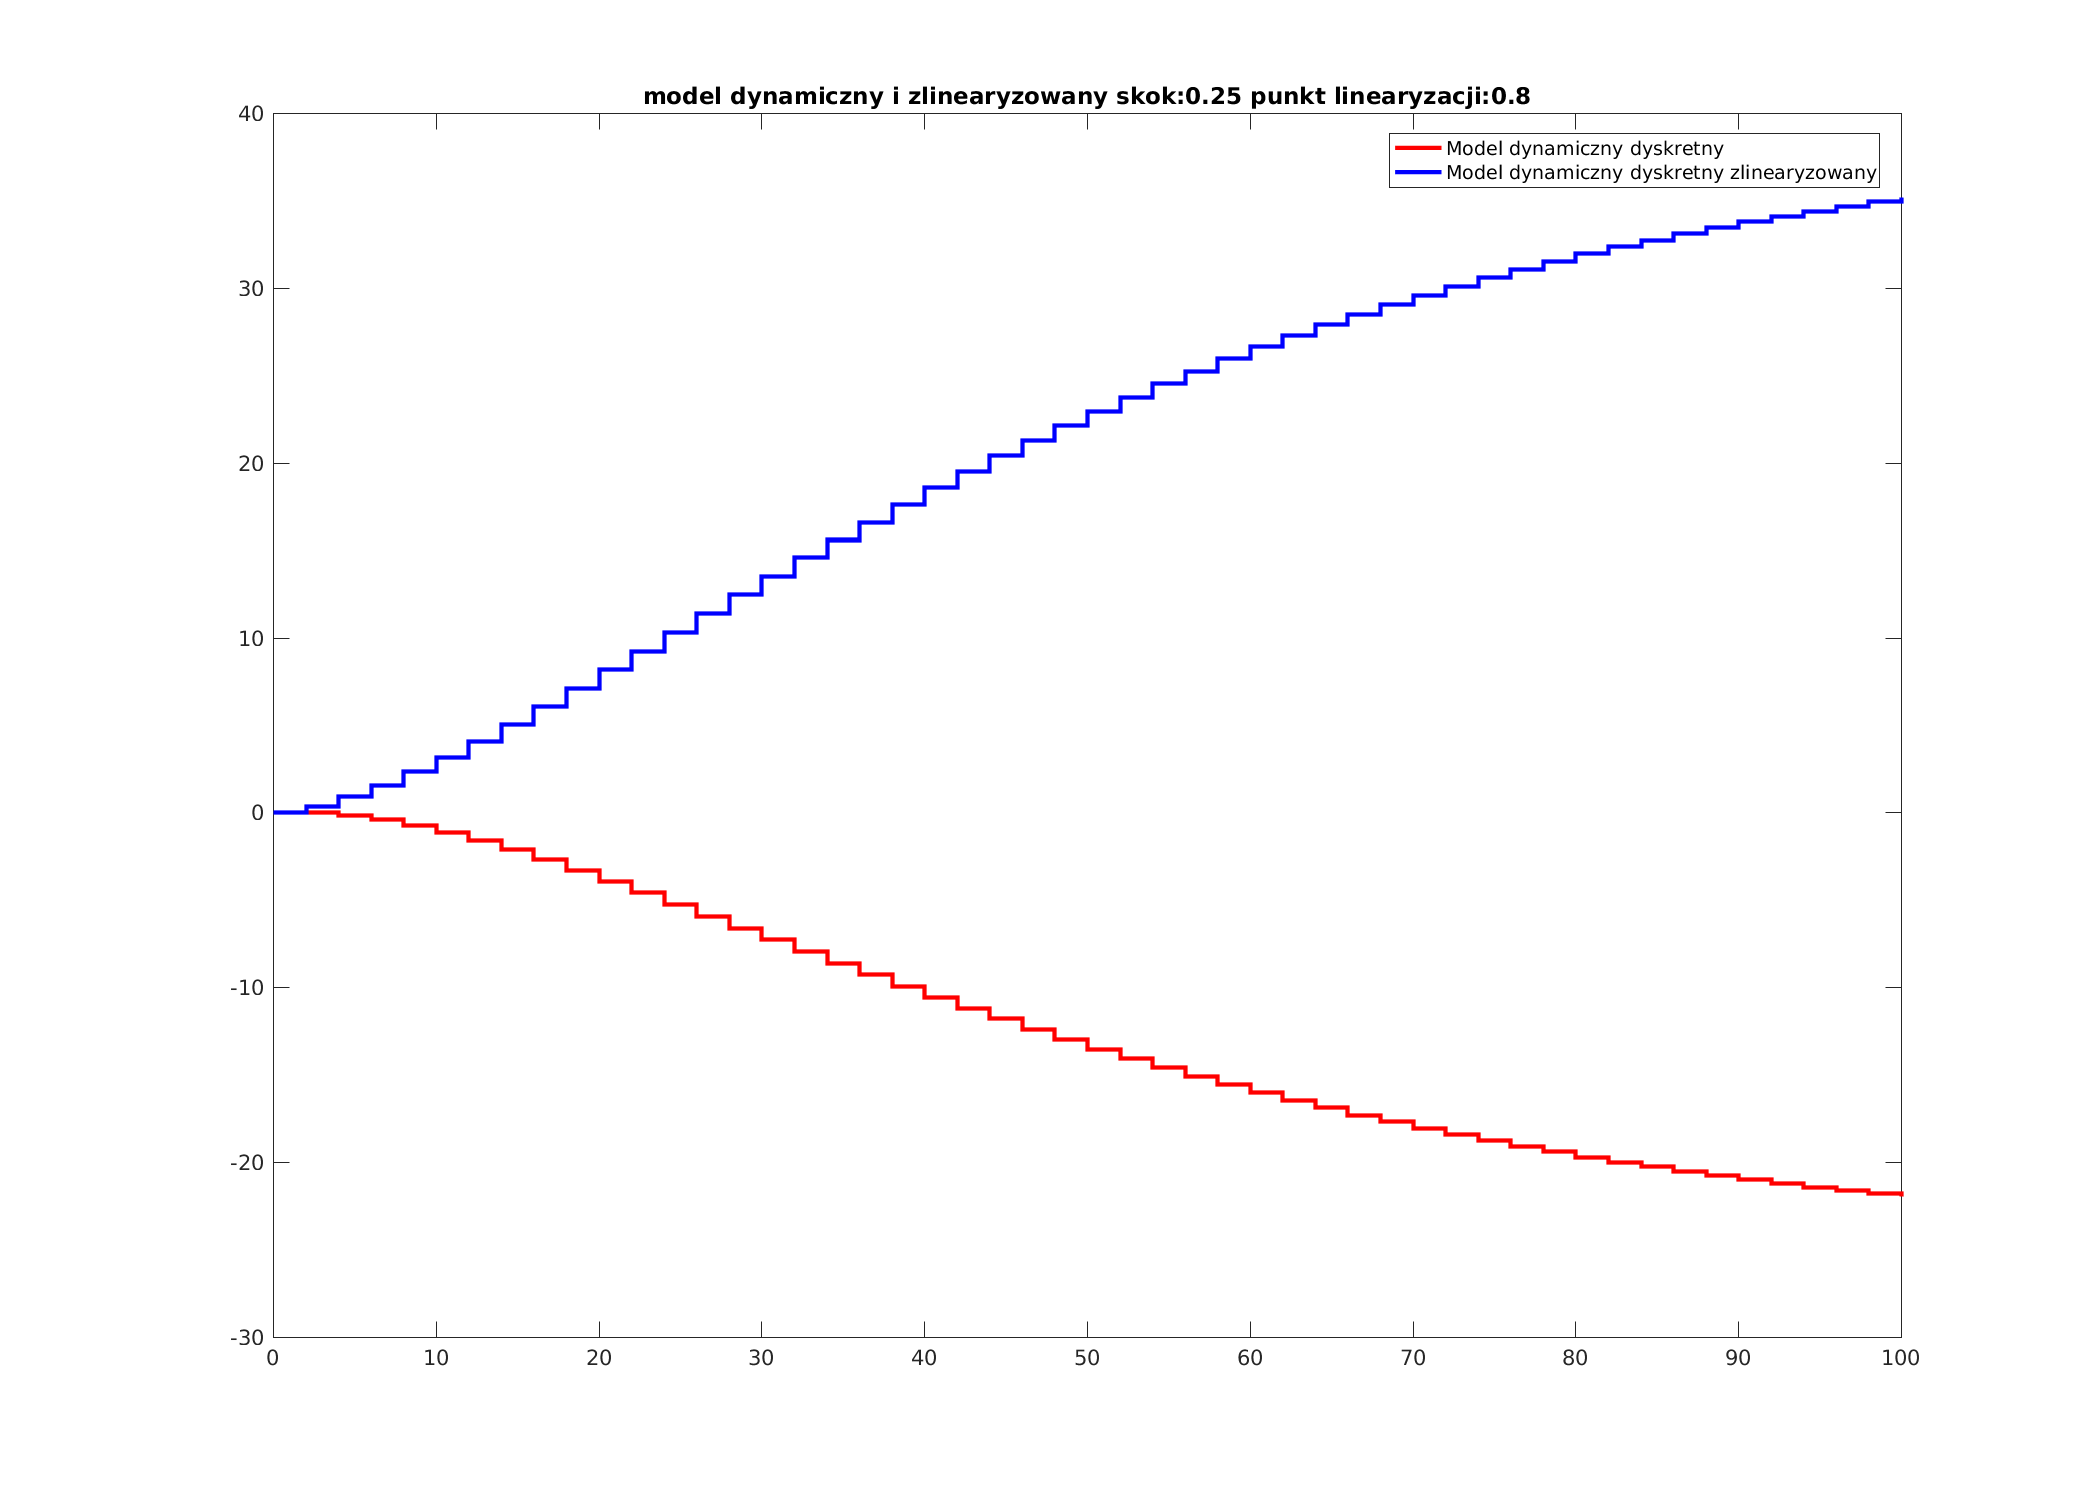
\includegraphics[scale=0.45]{9258.png}
\end{figure}

\begin{figure}[H]
\centering
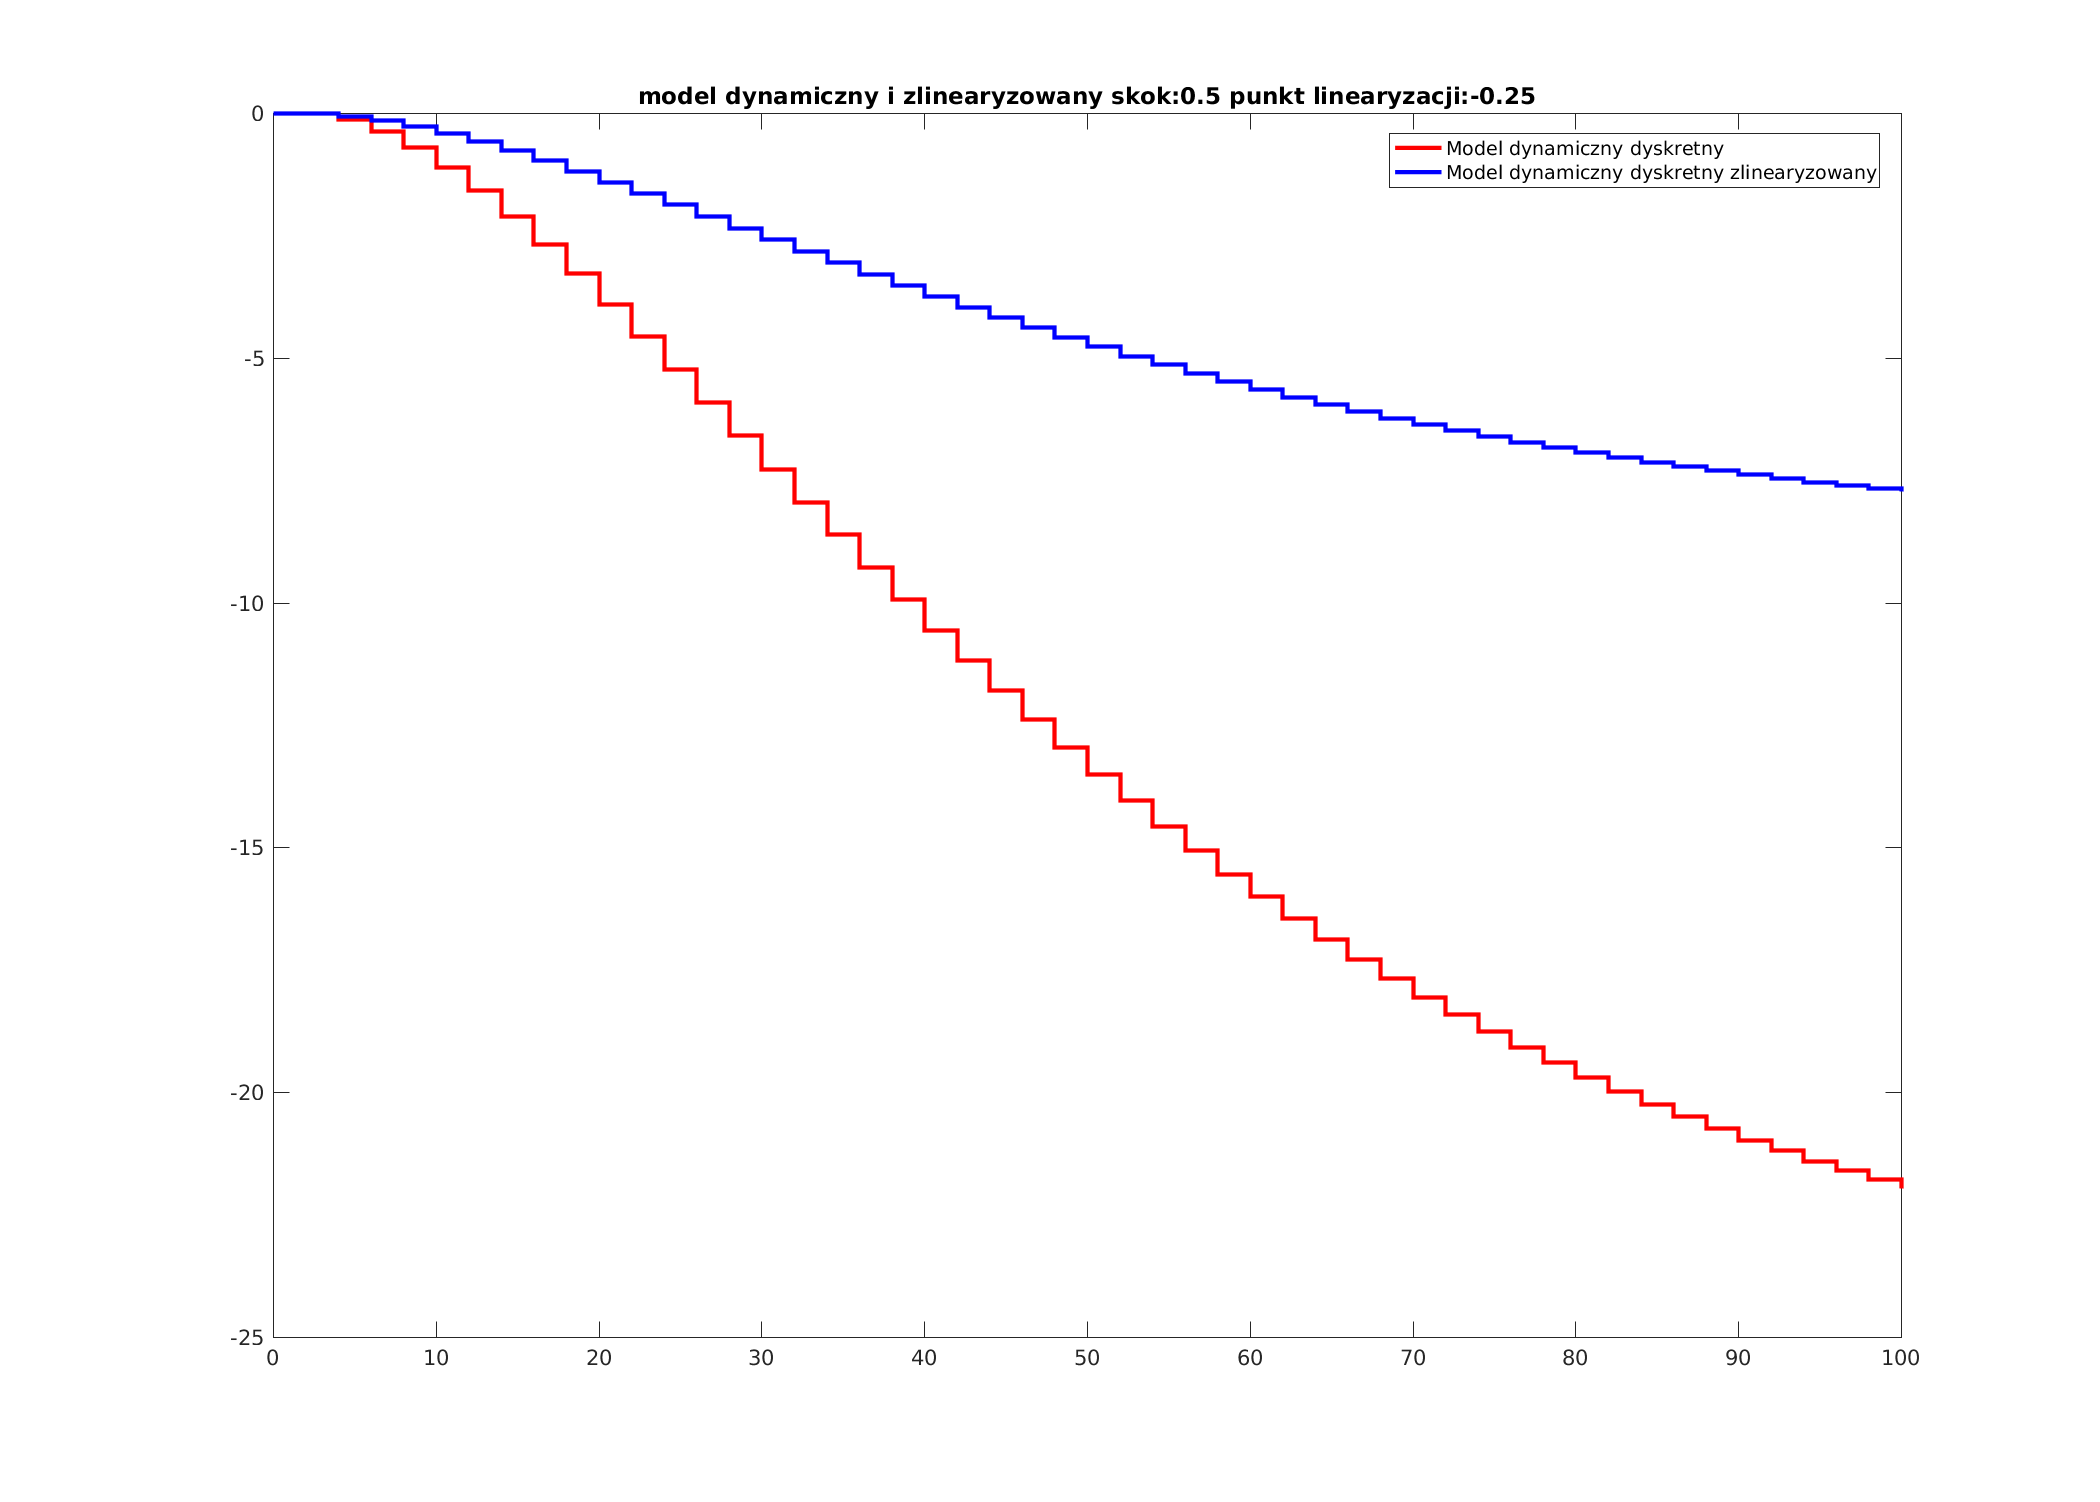
\includegraphics[scale=0.45]{95m25.png}
\end{figure}
\begin{figure}[H]
\centering
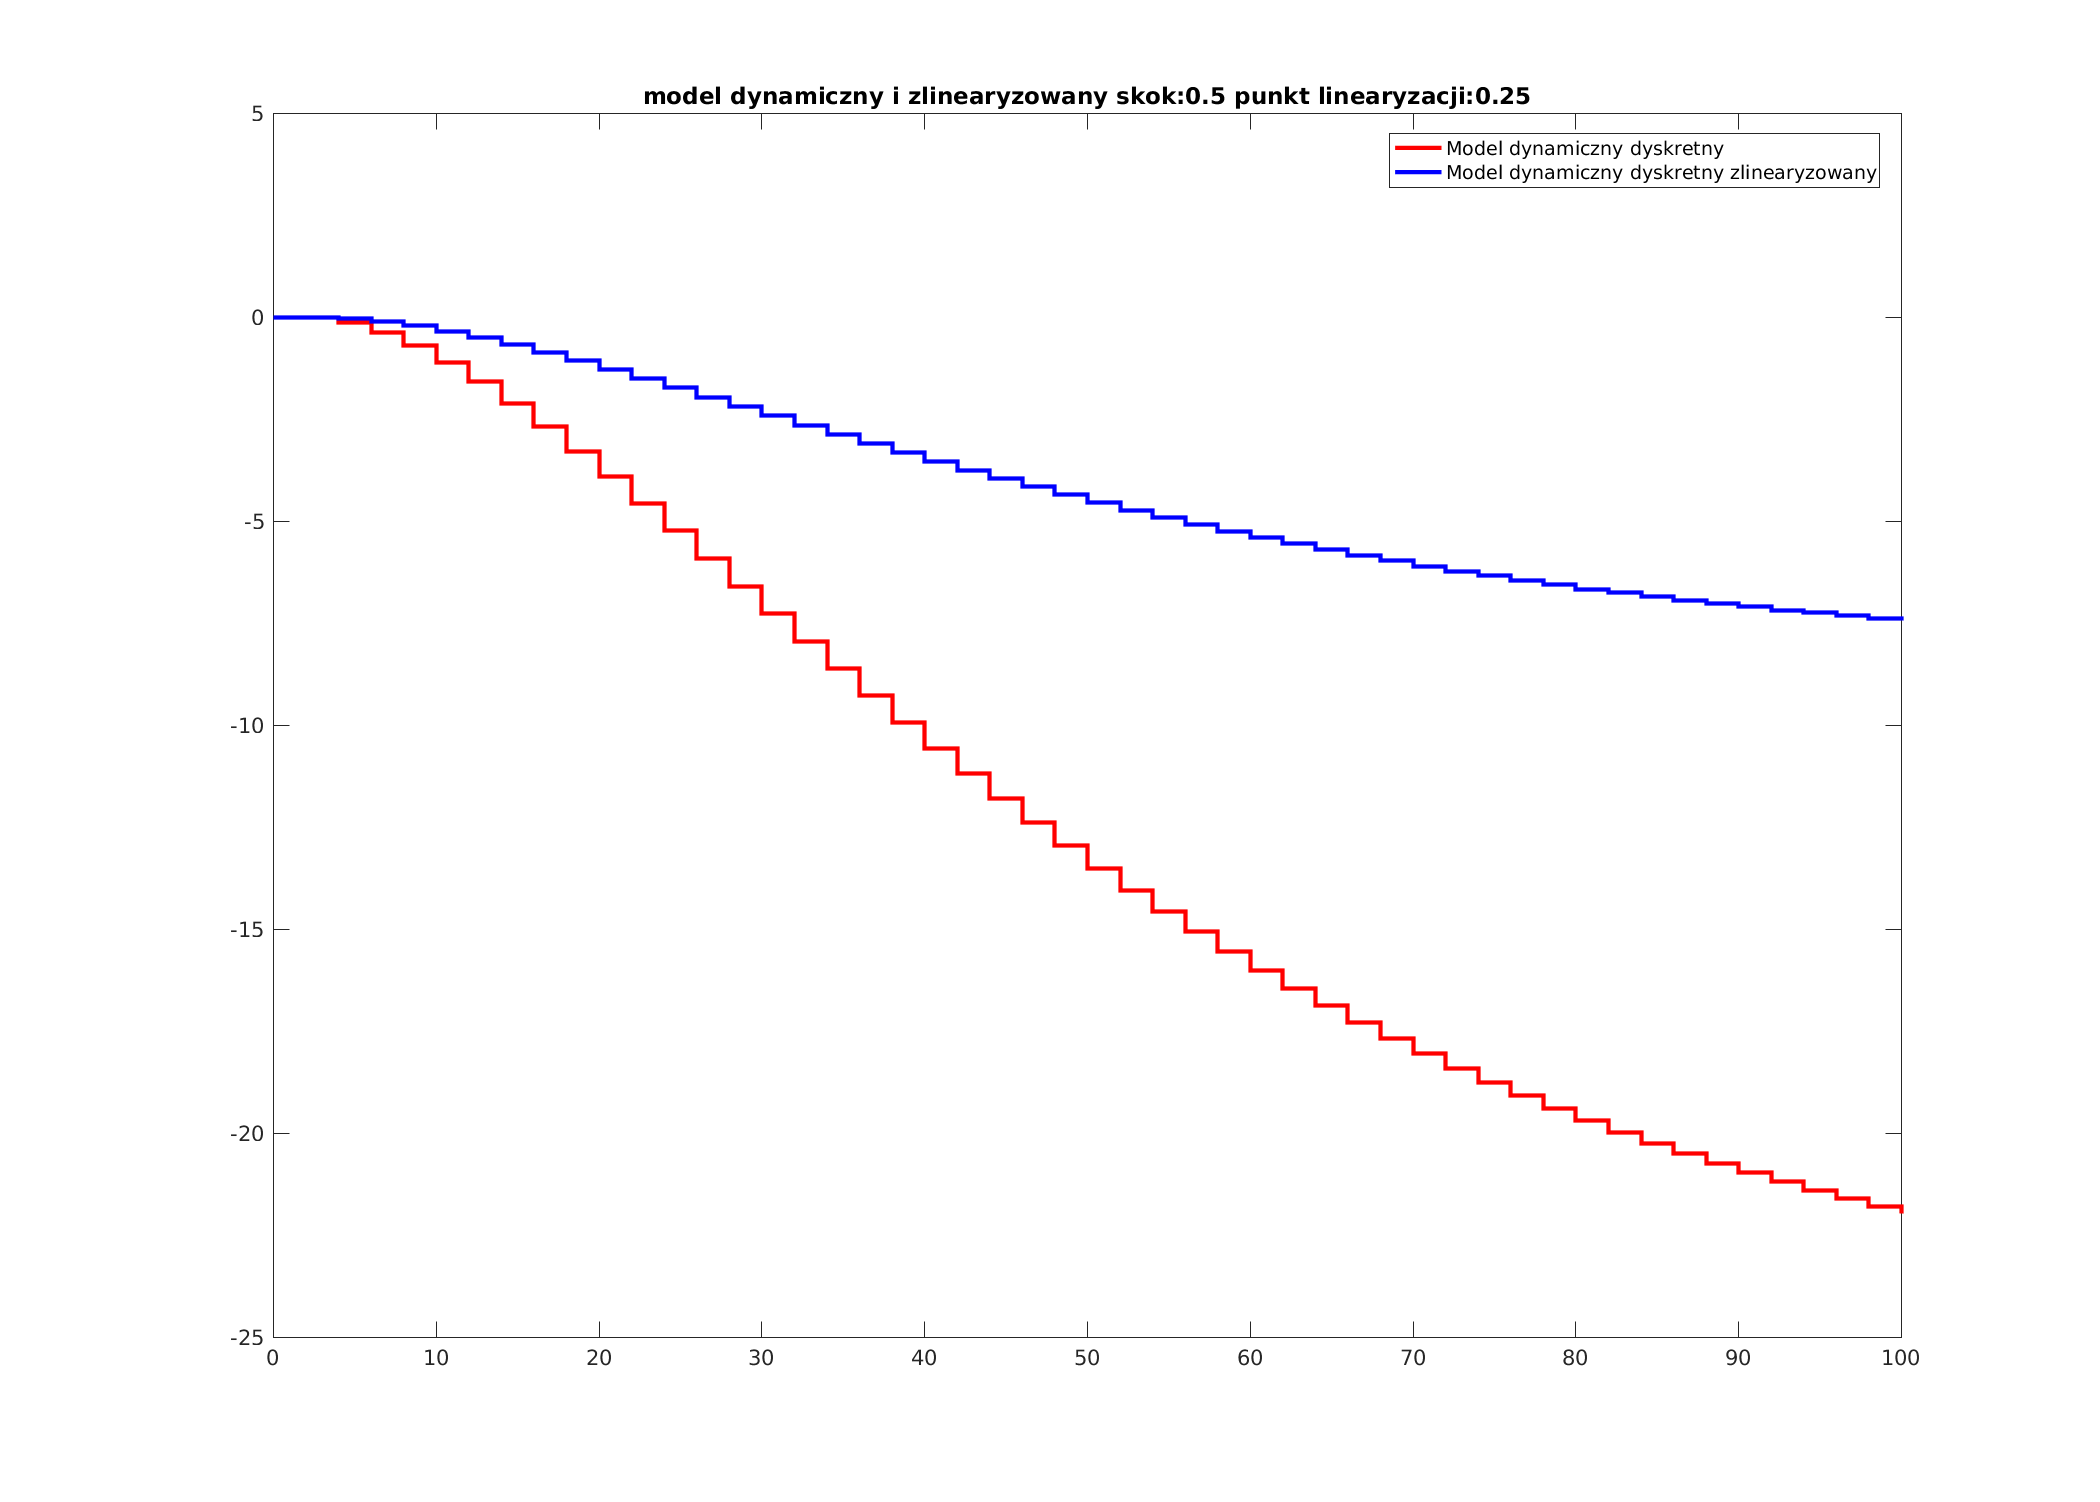
\includegraphics[scale=0.45]{9525.png}
\end{figure}
\begin{figure}[H]
\centering
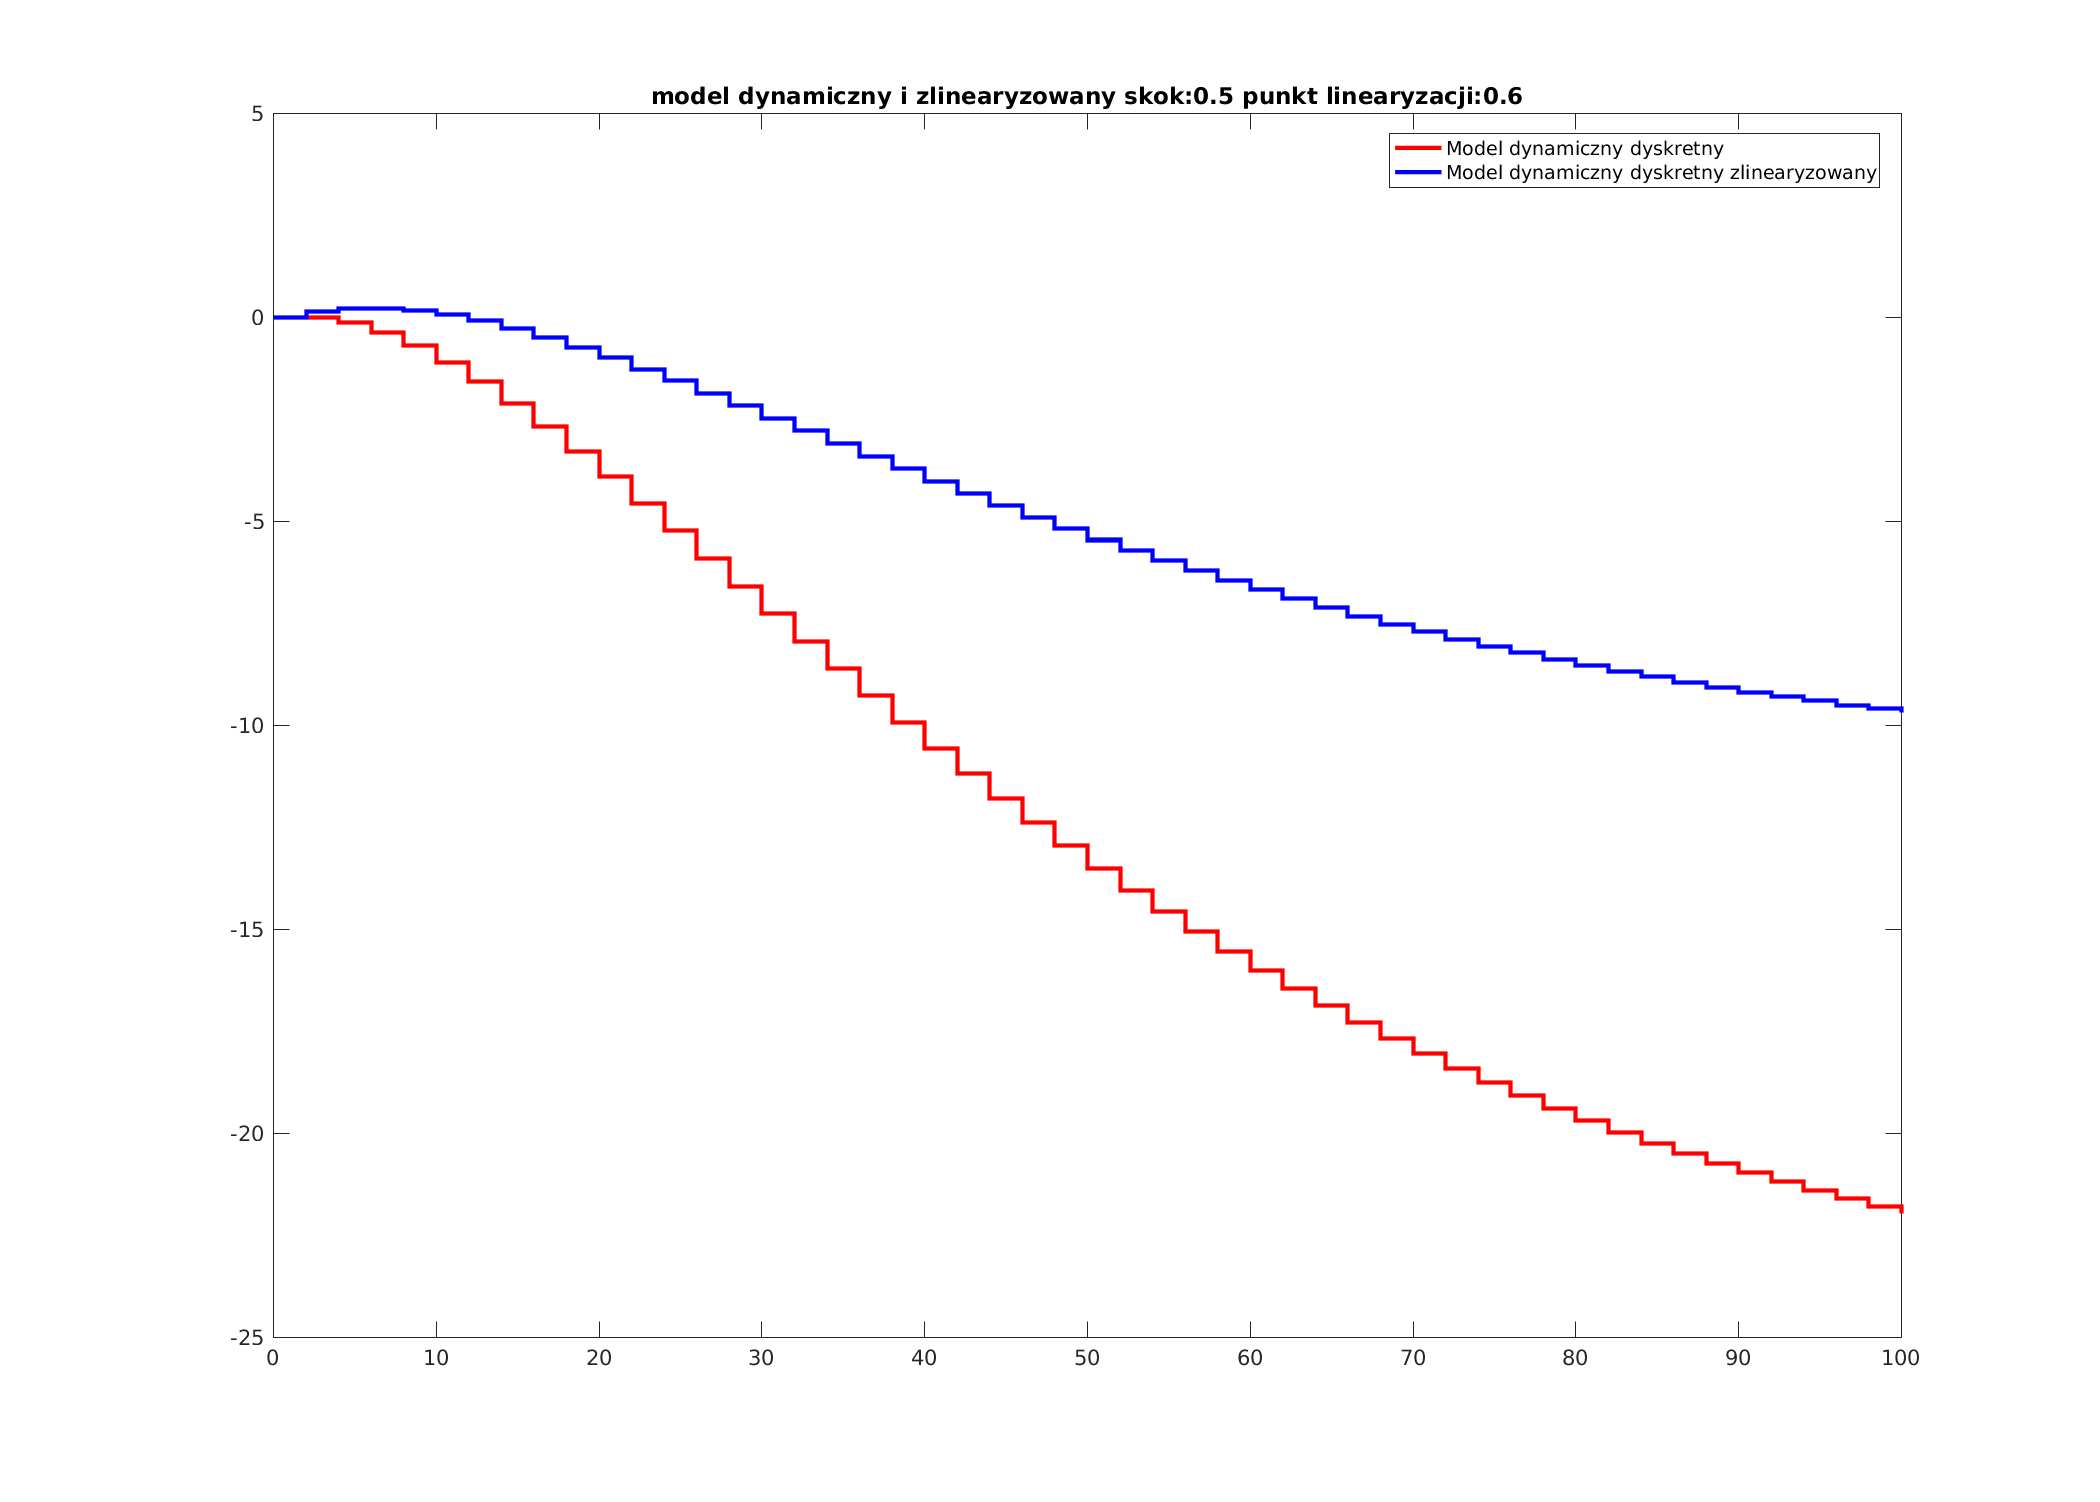
\includegraphics[scale=0.45]{956.png}
\end{figure}
\begin{figure}[H]
\centering
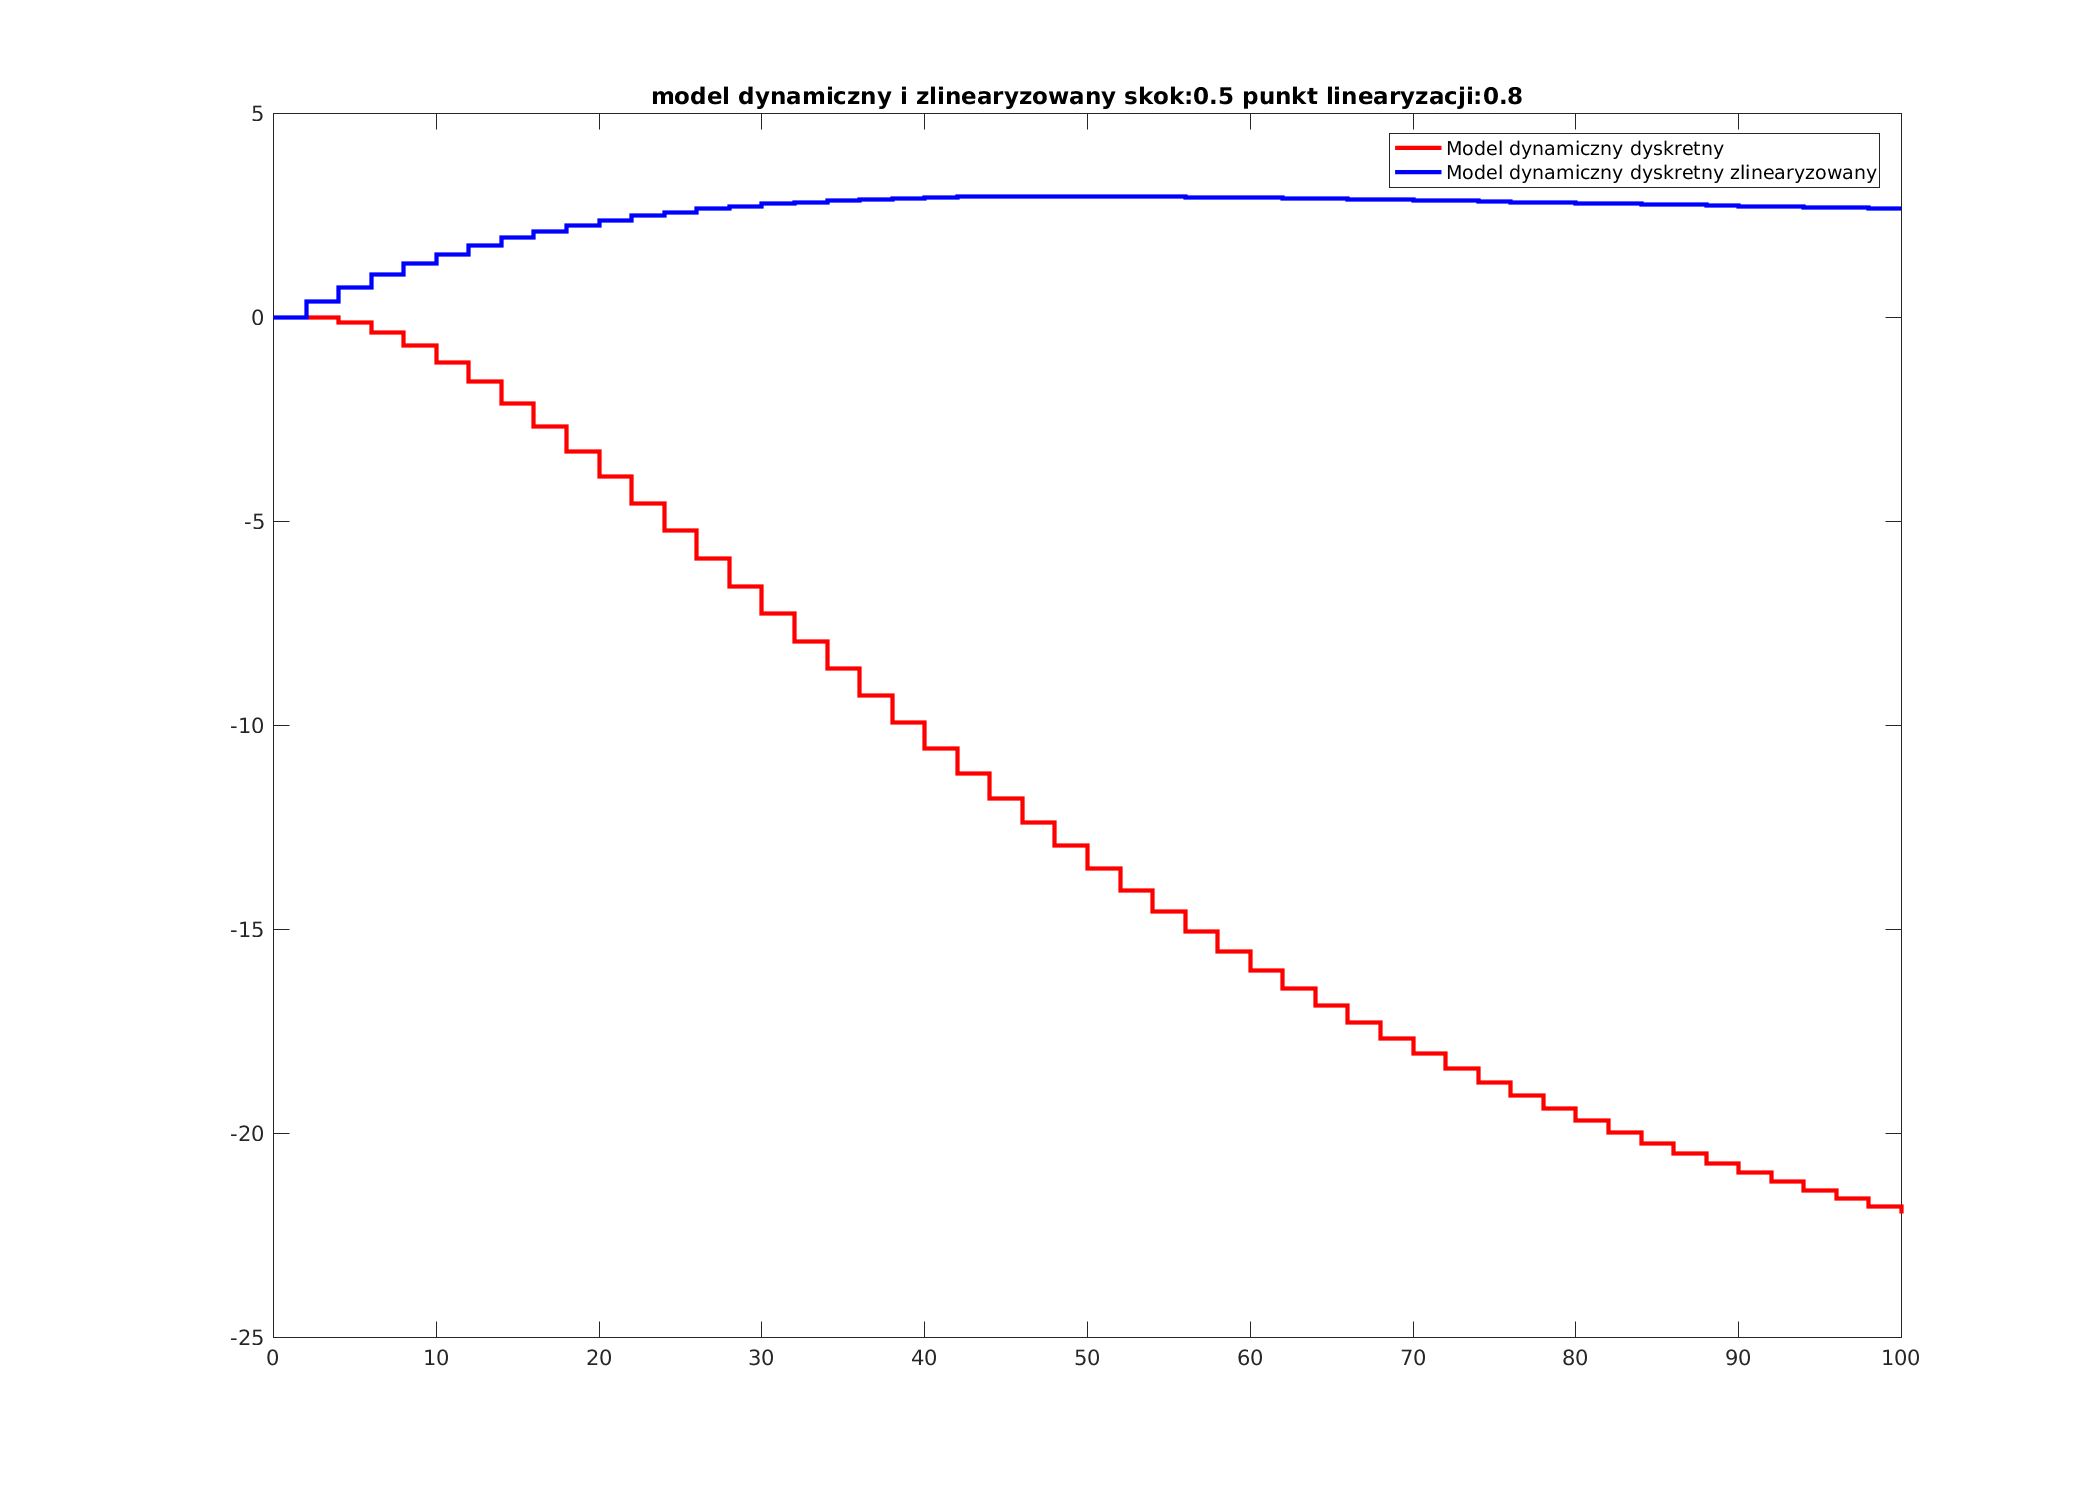
\includegraphics[scale=0.45]{958.png}
\end{figure}

\begin{figure}[H]
\centering
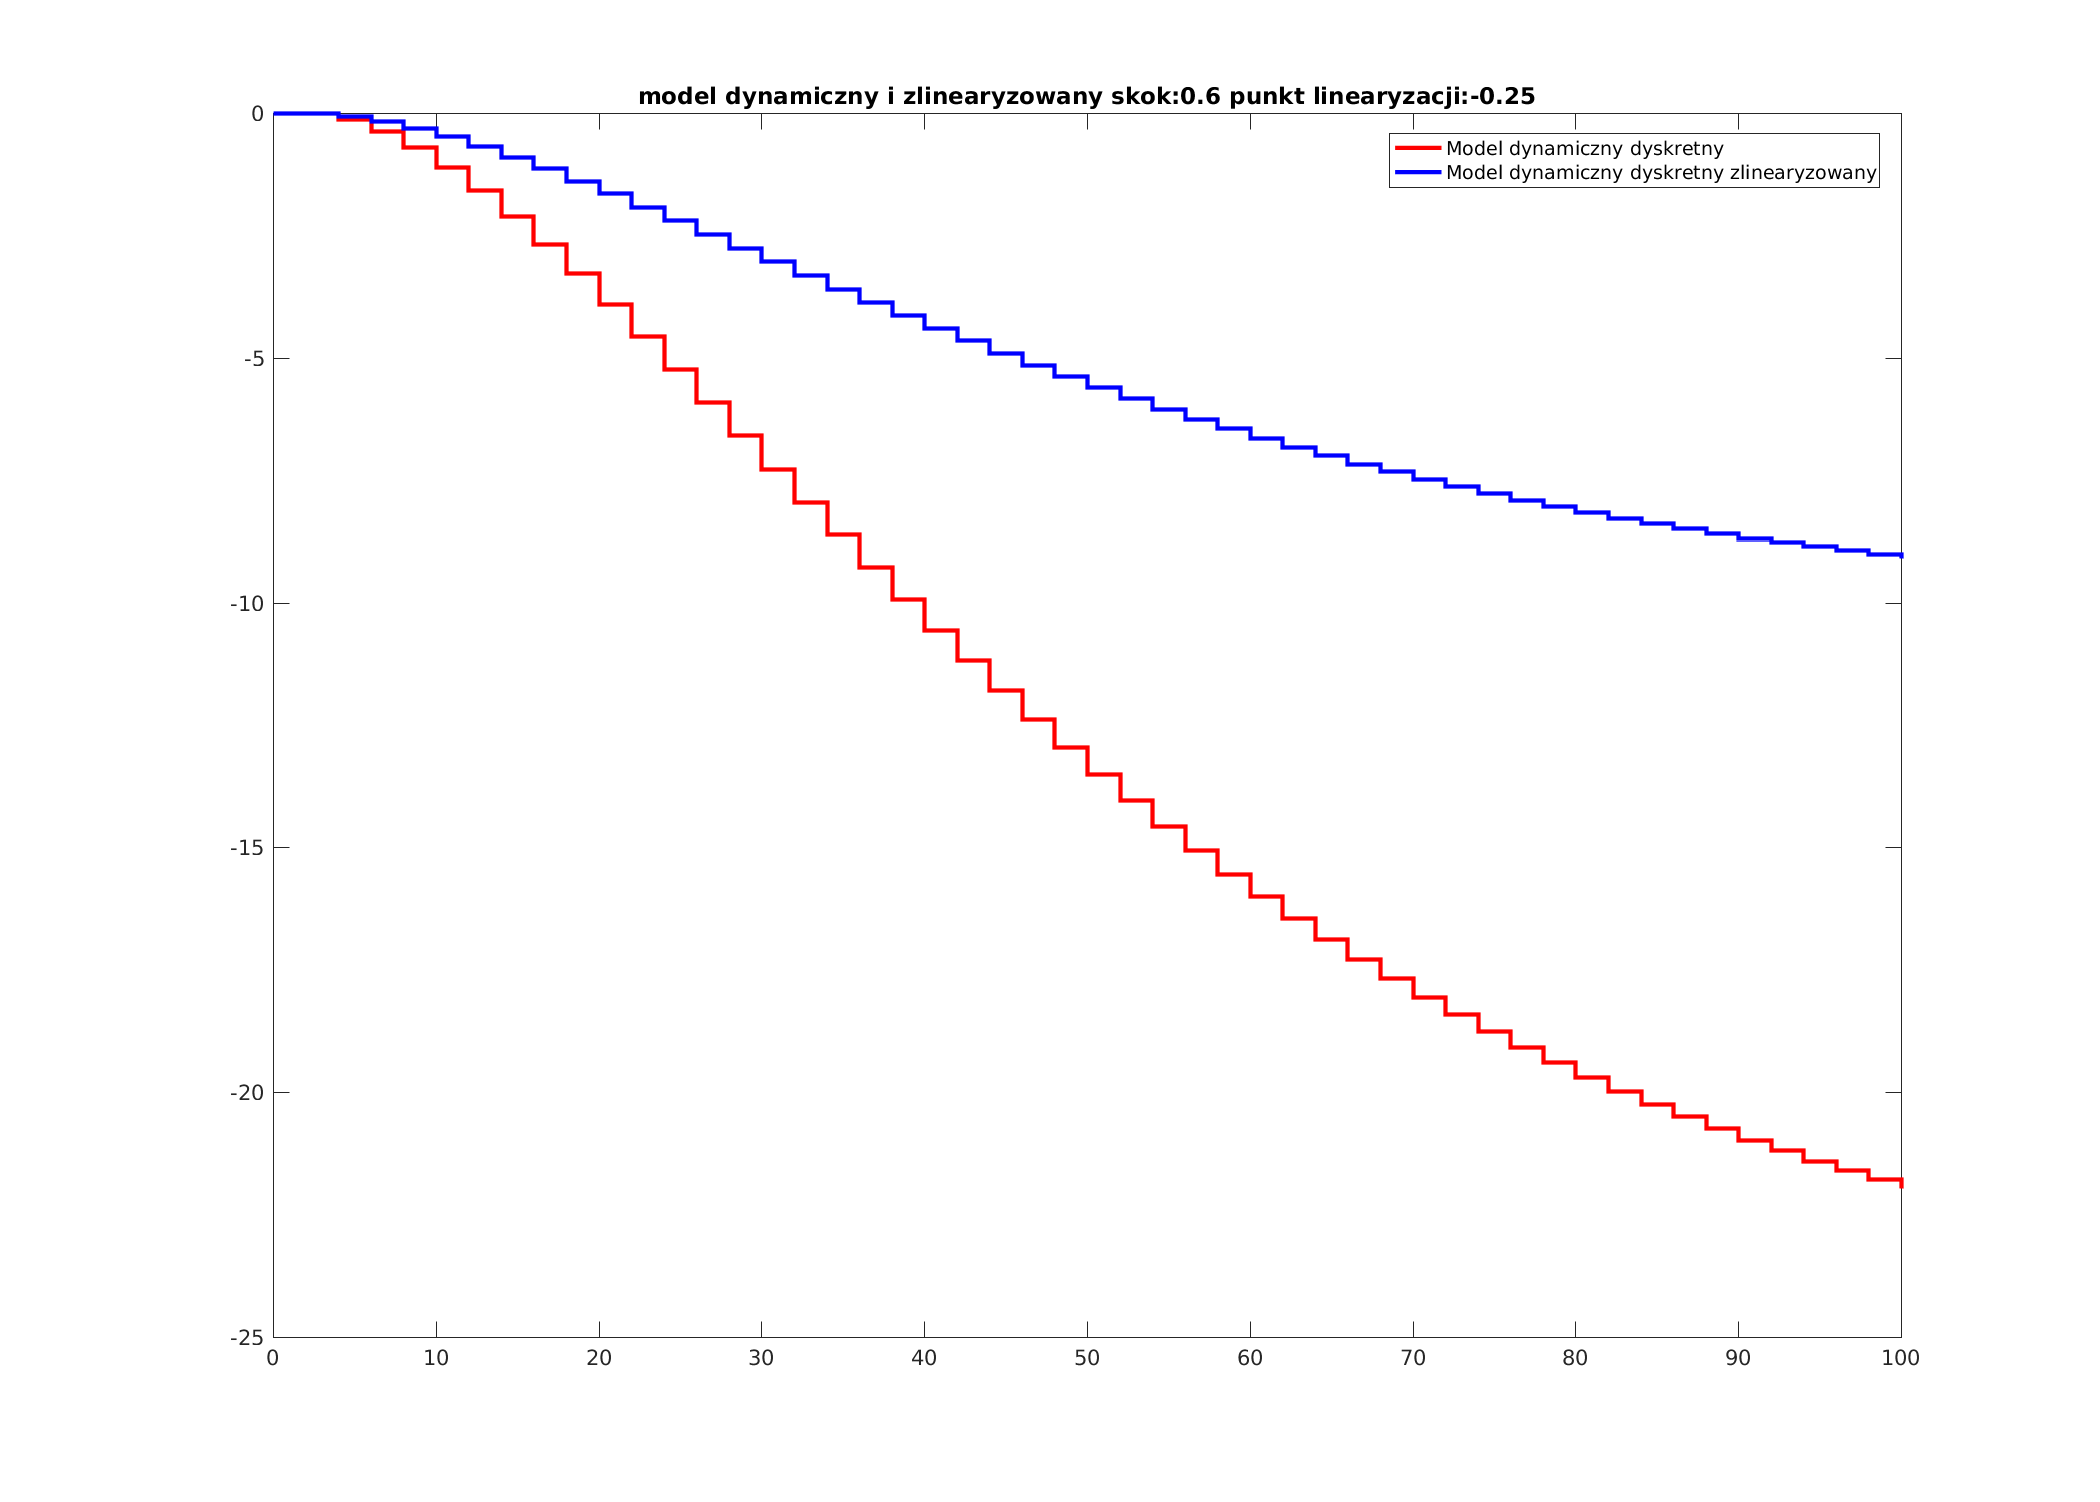
\includegraphics[scale=0.45]{96m25.png}
\end{figure}
\begin{figure}[H]
\centering
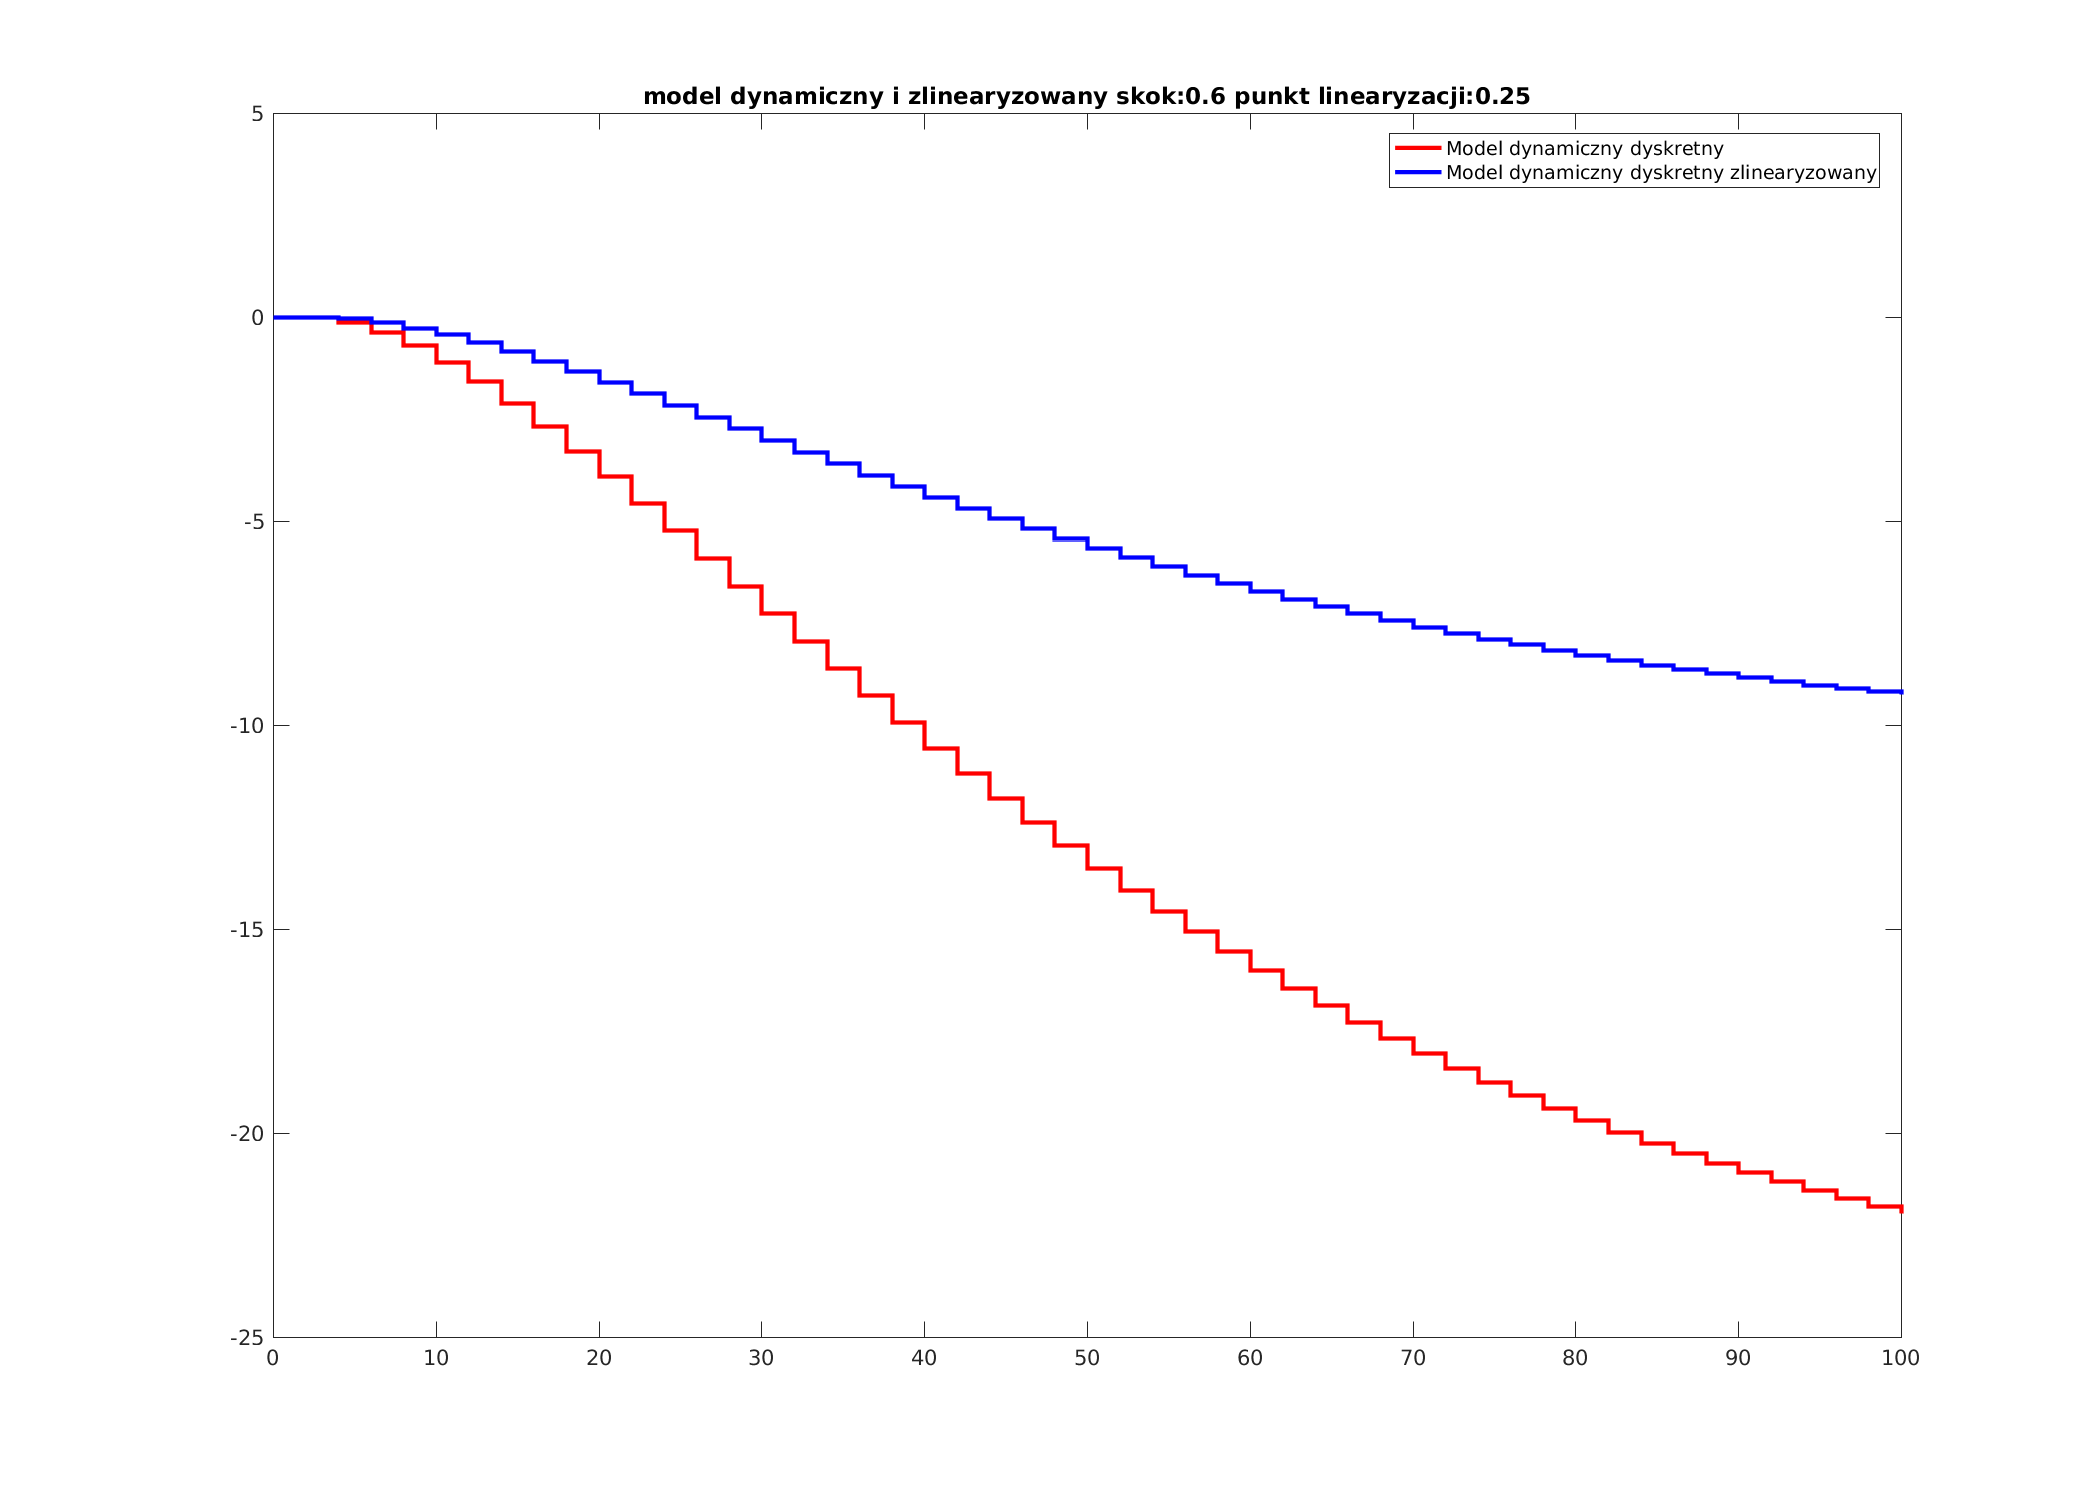
\includegraphics[scale=0.45]{9625.png}
\end{figure}
\begin{figure}[H]
\centering
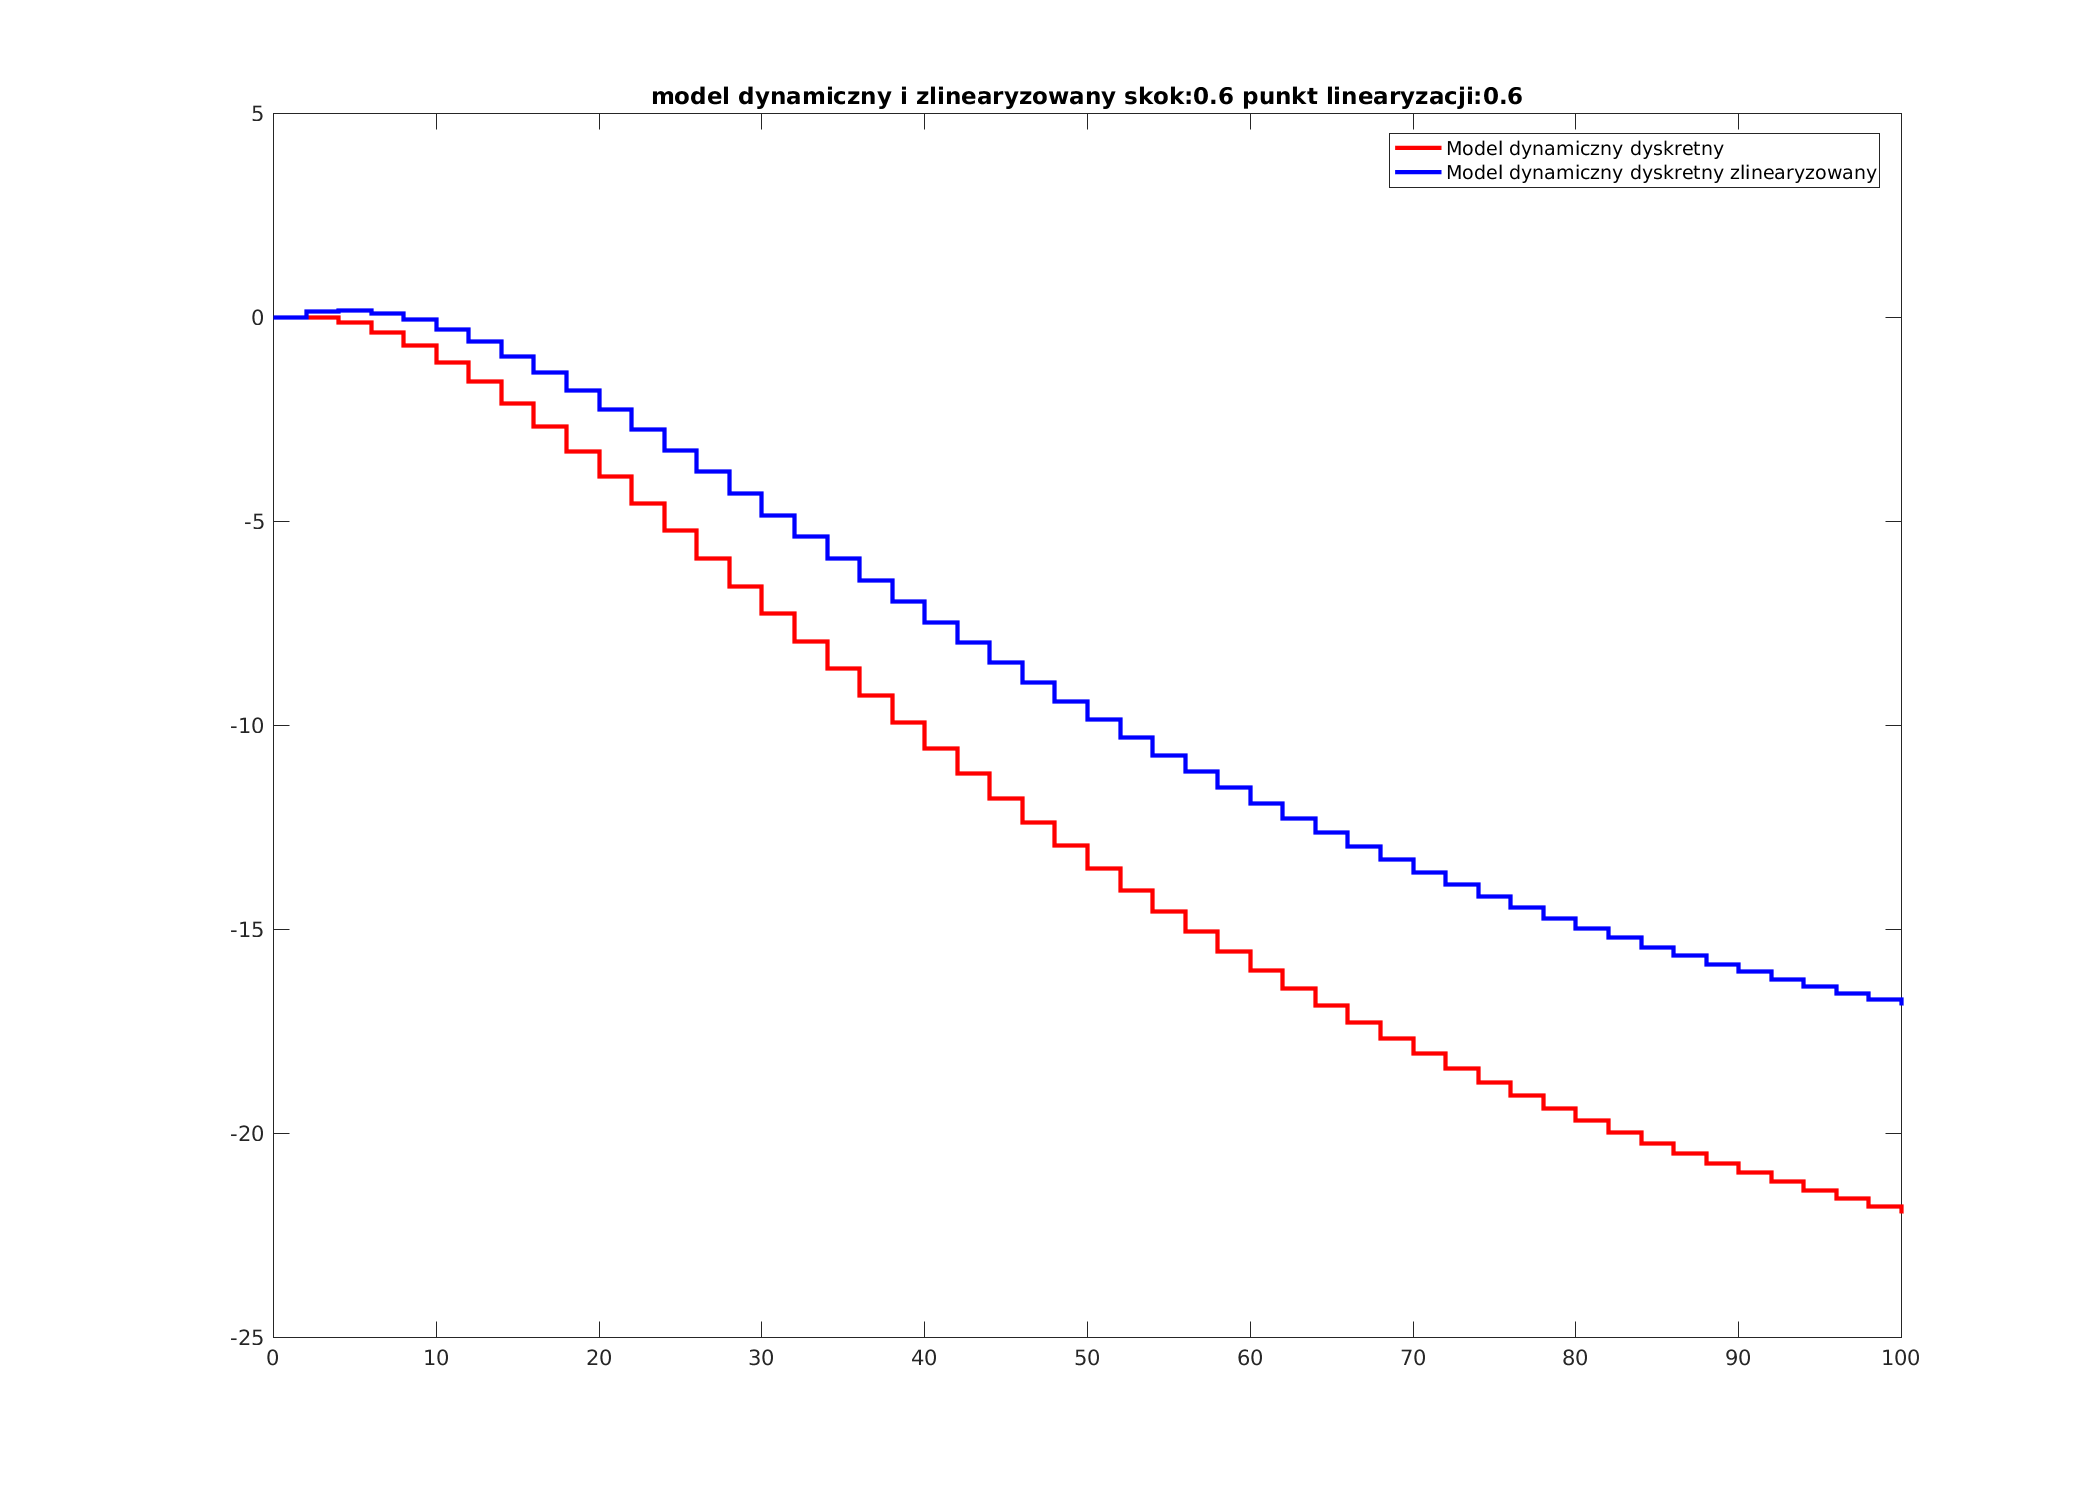
\includegraphics[scale=0.45]{966.png}
\end{figure}
\begin{figure}[H]
\centering
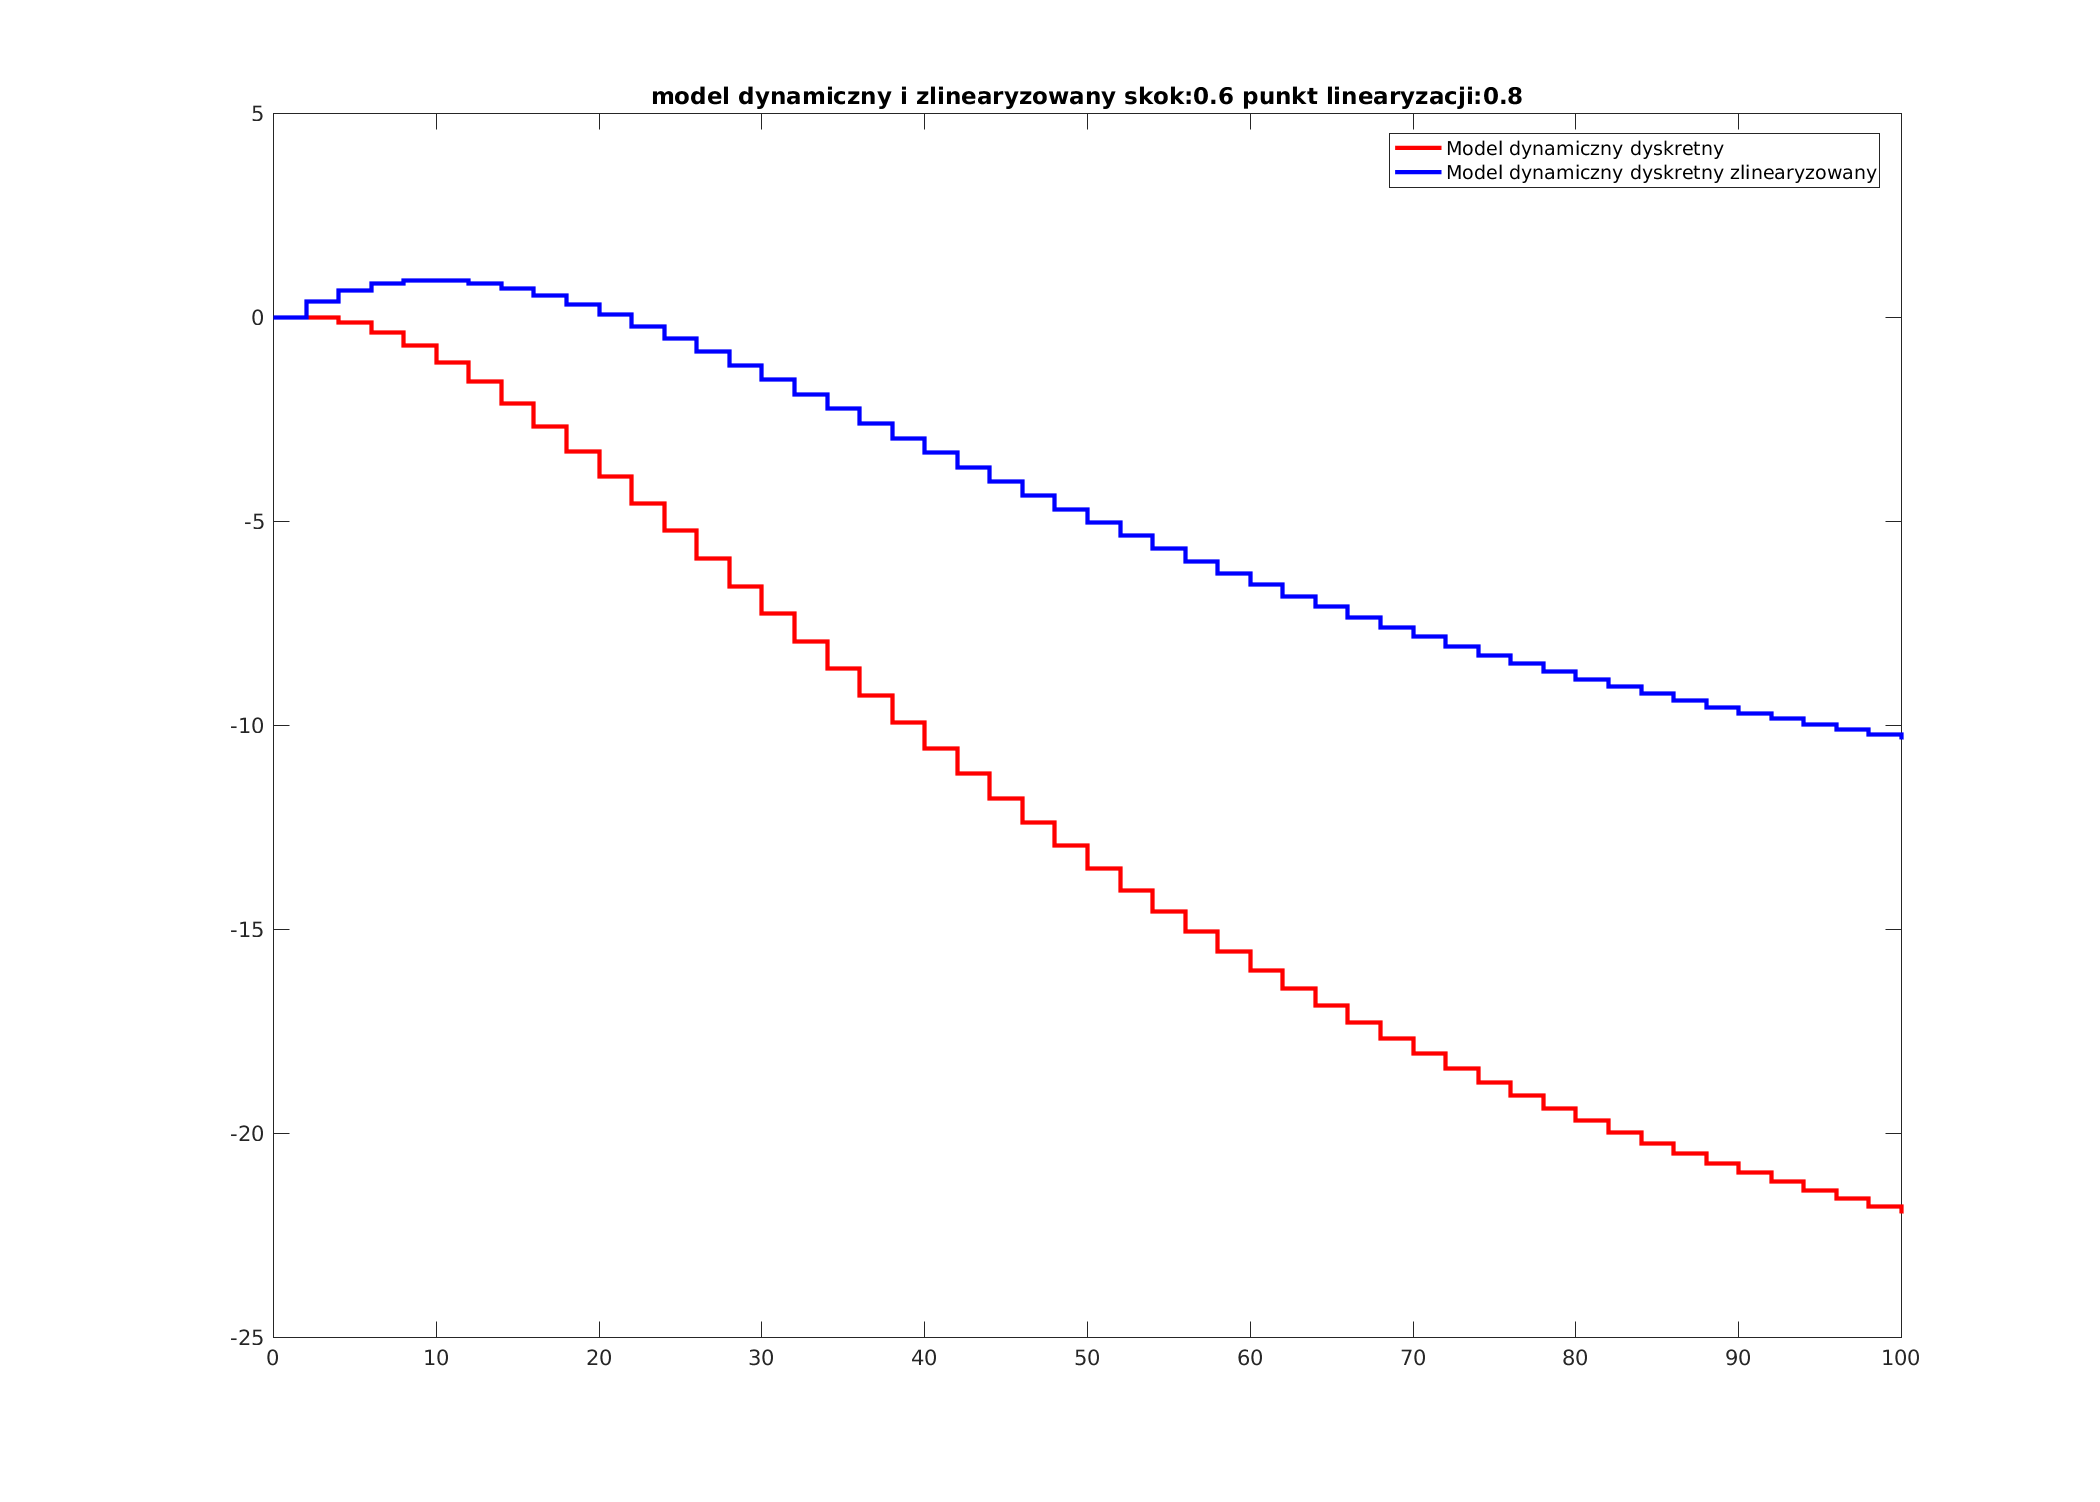
\includegraphics[scale=0.45]{968.png}
\end{figure}

\begin{figure}[H]
\centering
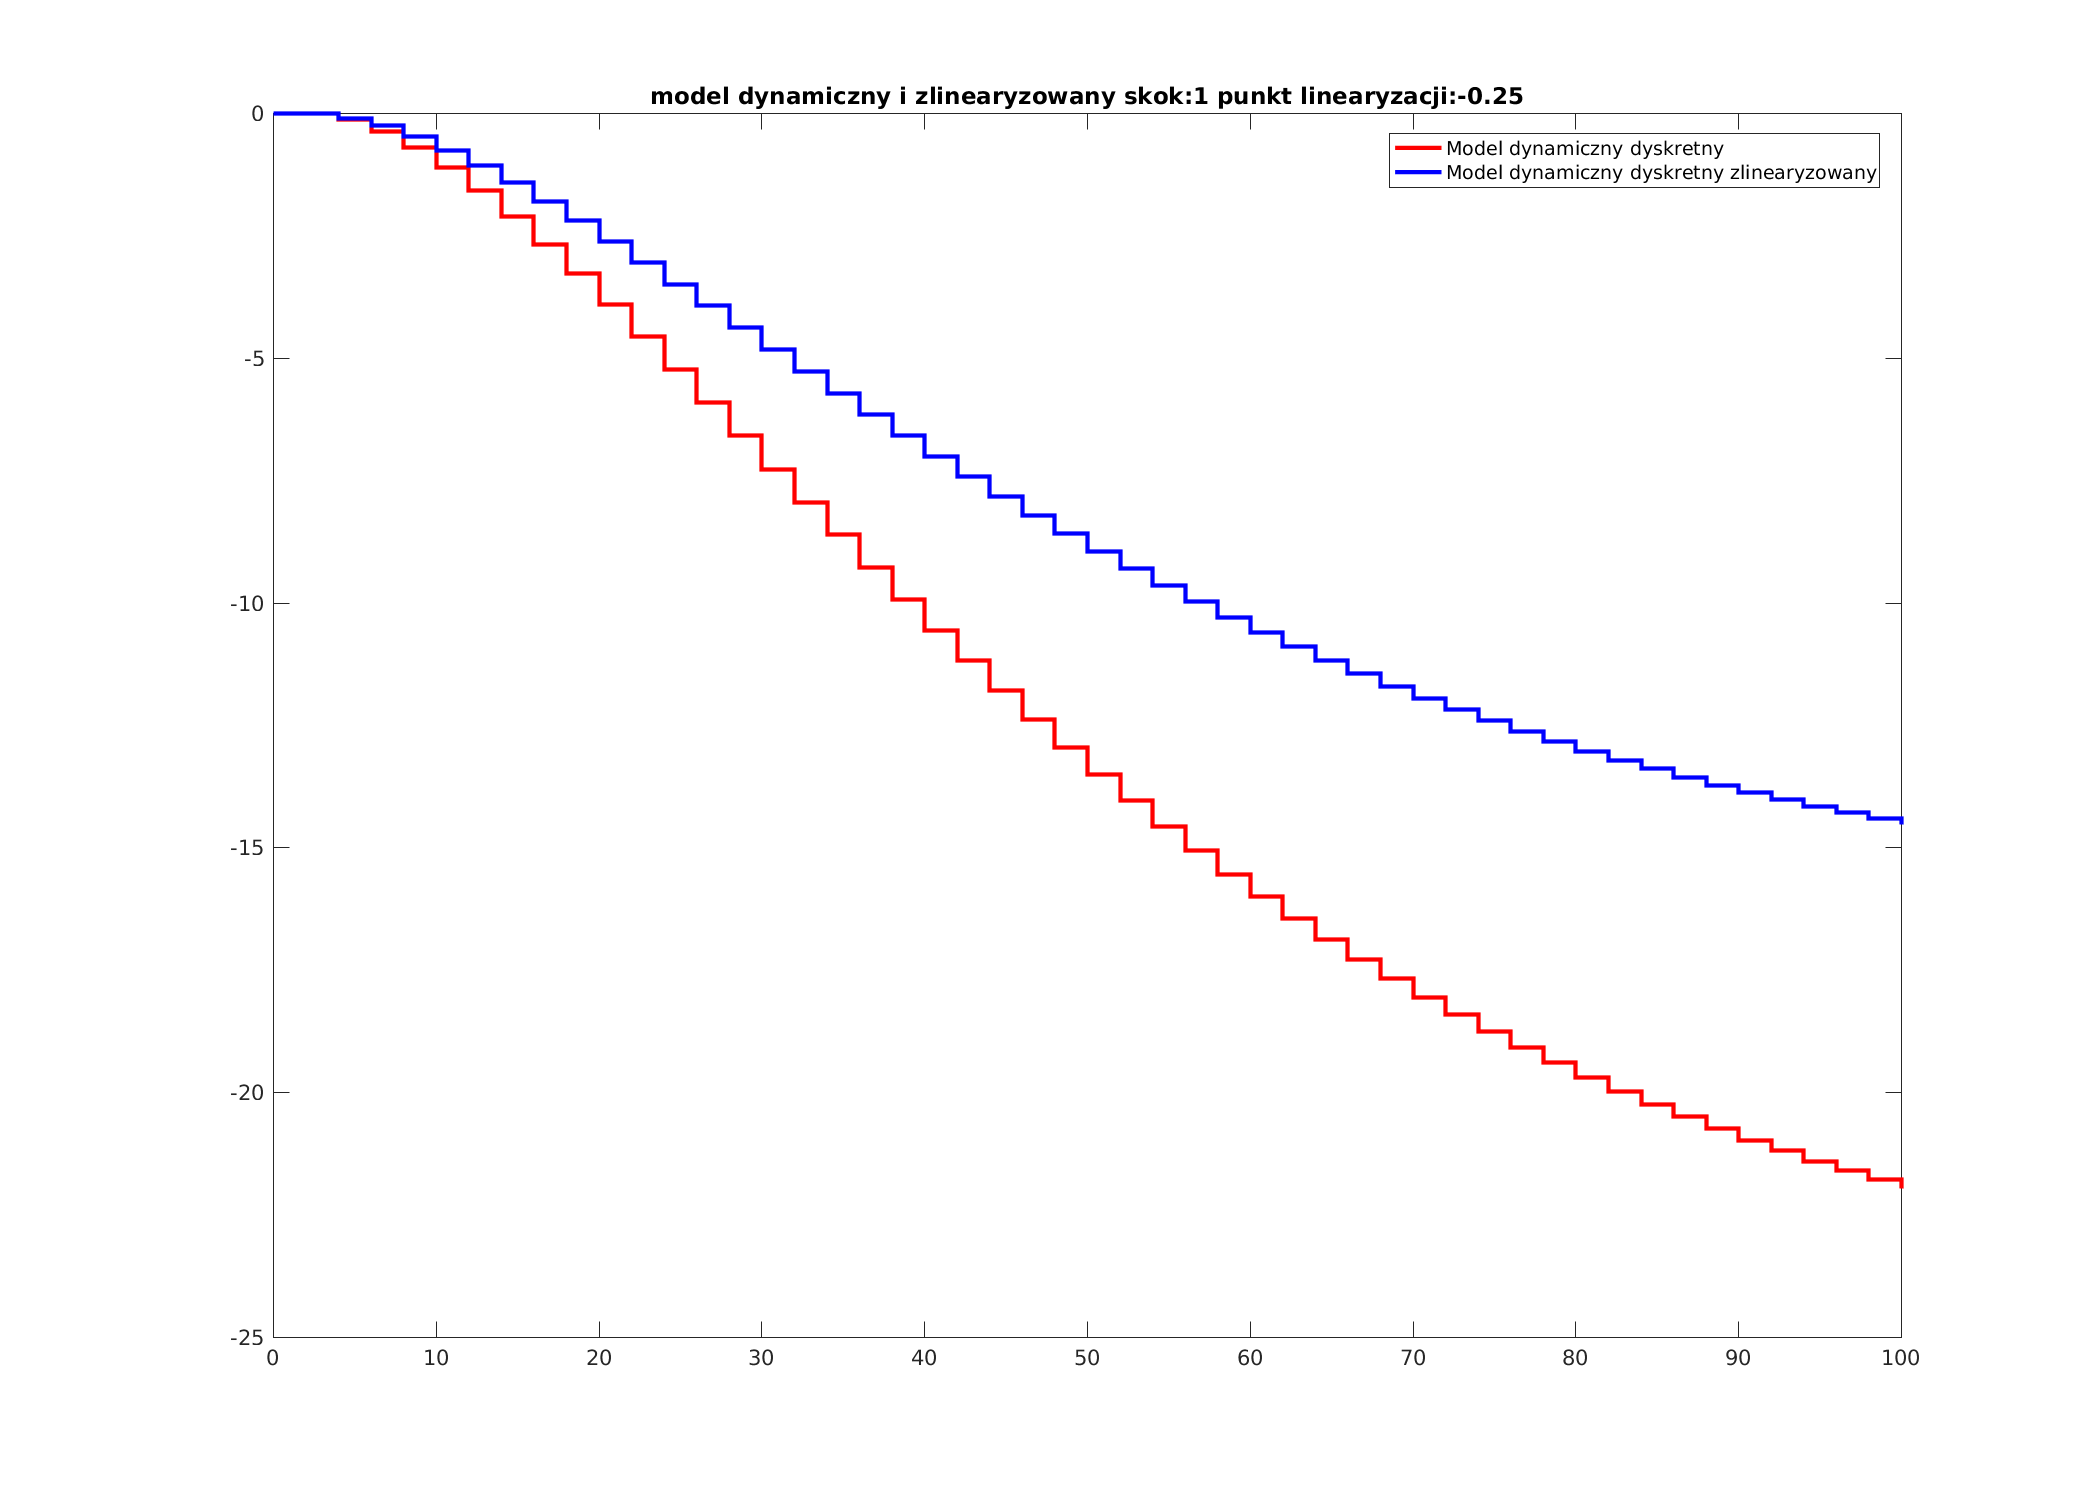
\includegraphics[scale=0.45]{91m25.png}
\end{figure}
\begin{figure}[H]
\centering
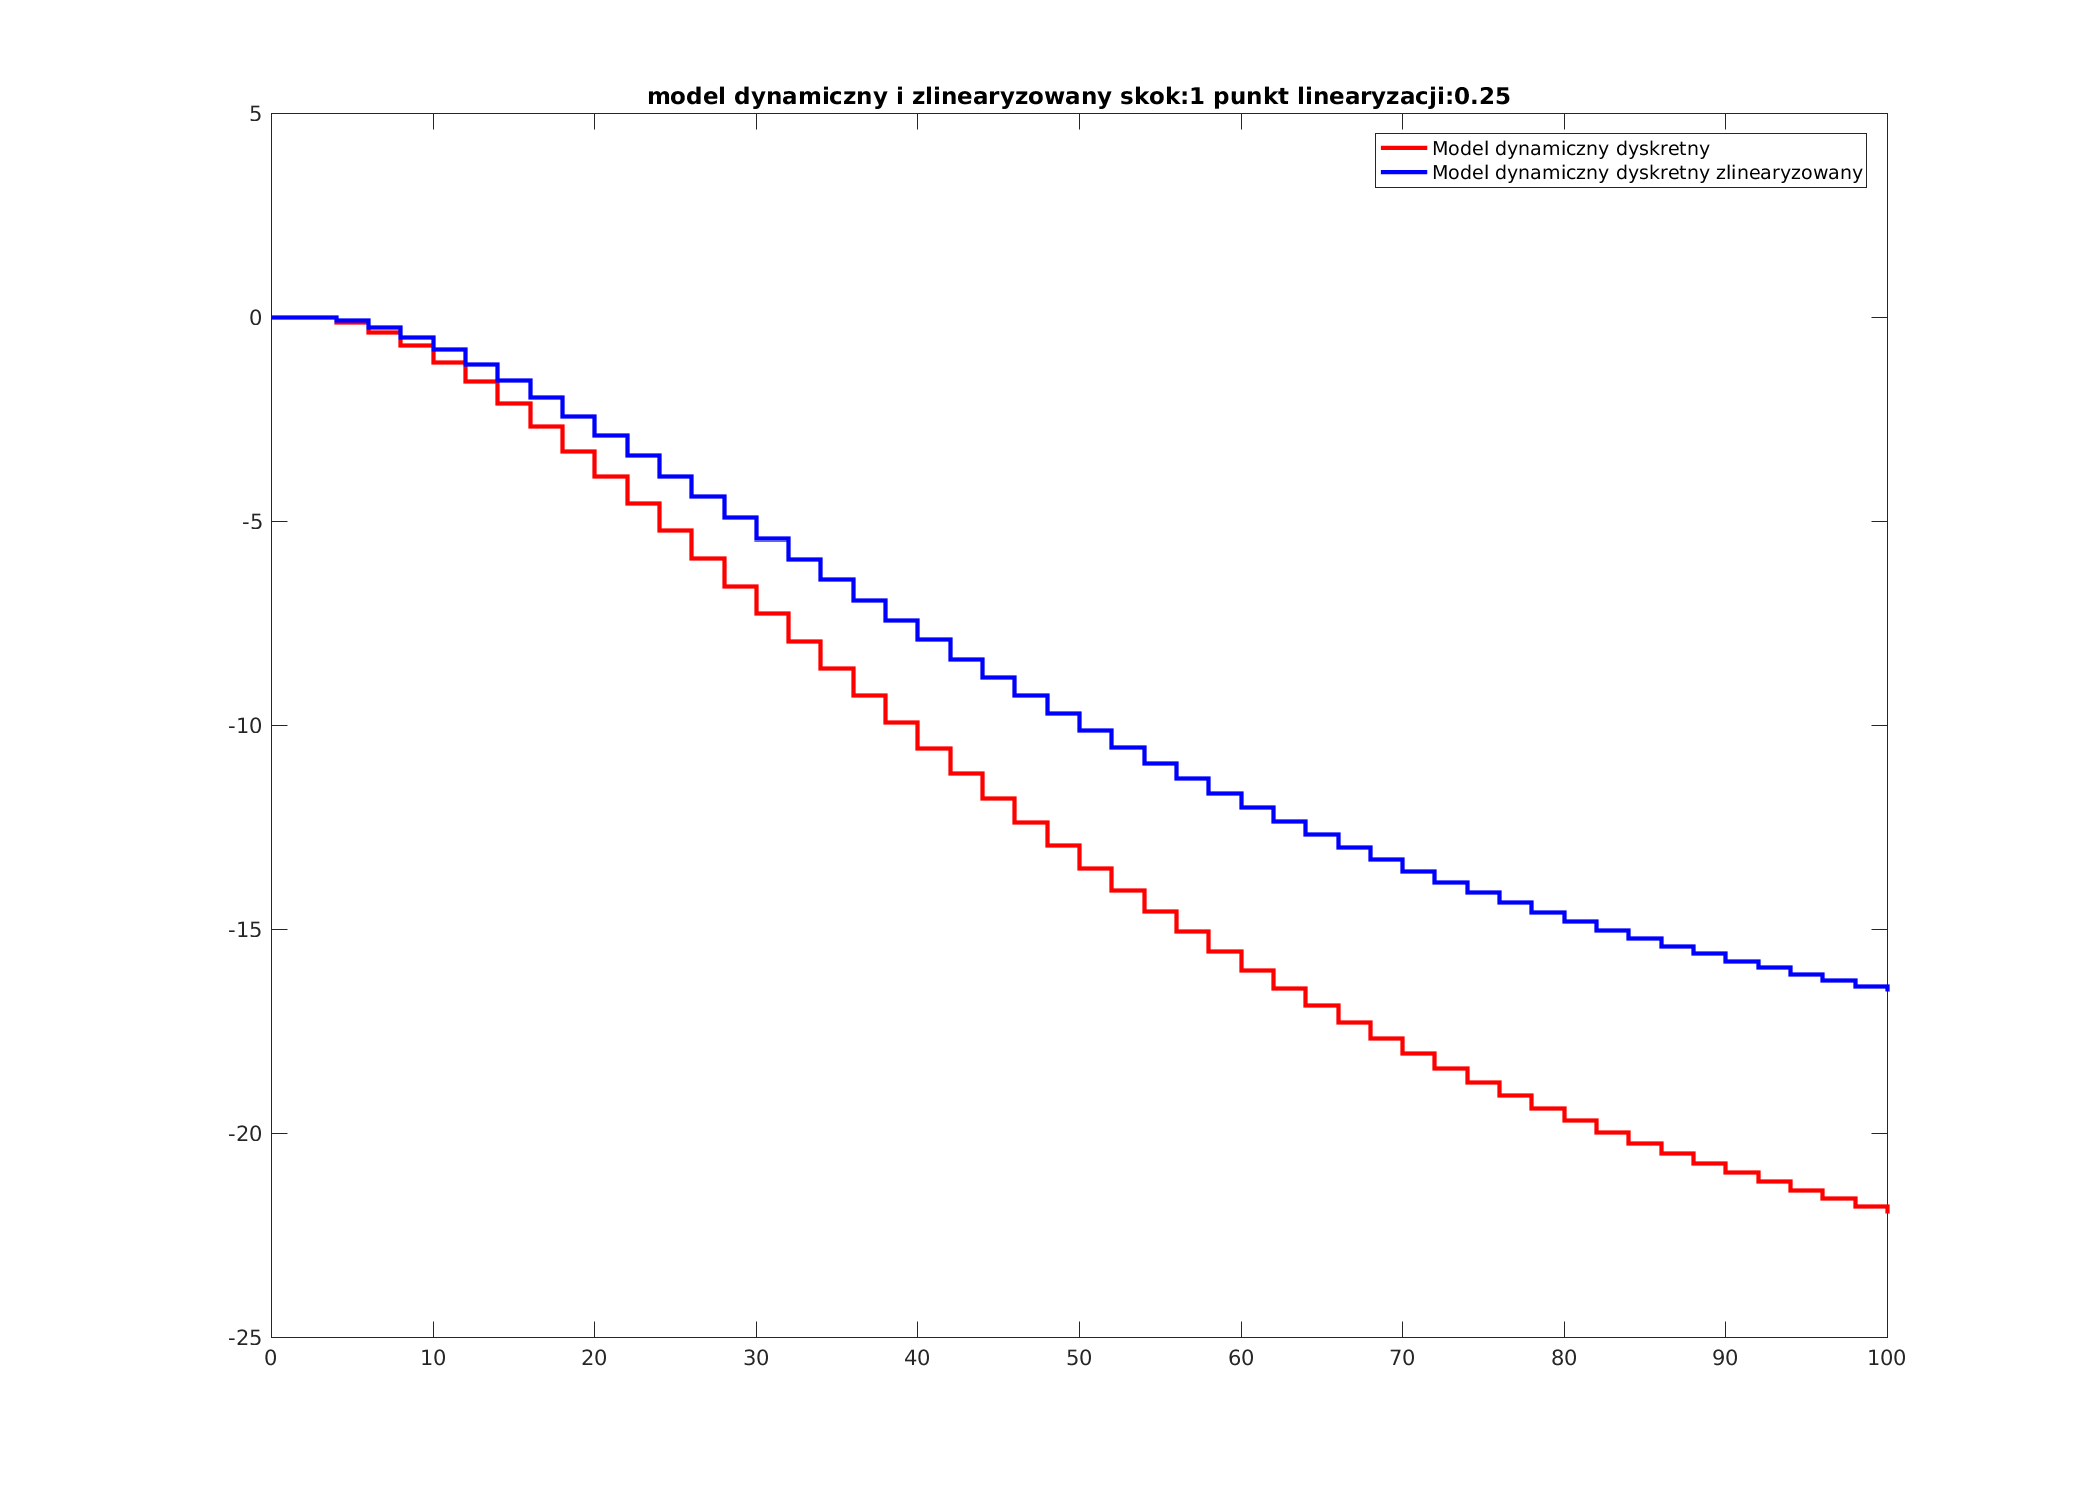
\includegraphics[scale=0.45]{9125.png}
\end{figure}
\begin{figure}[H]
\centering
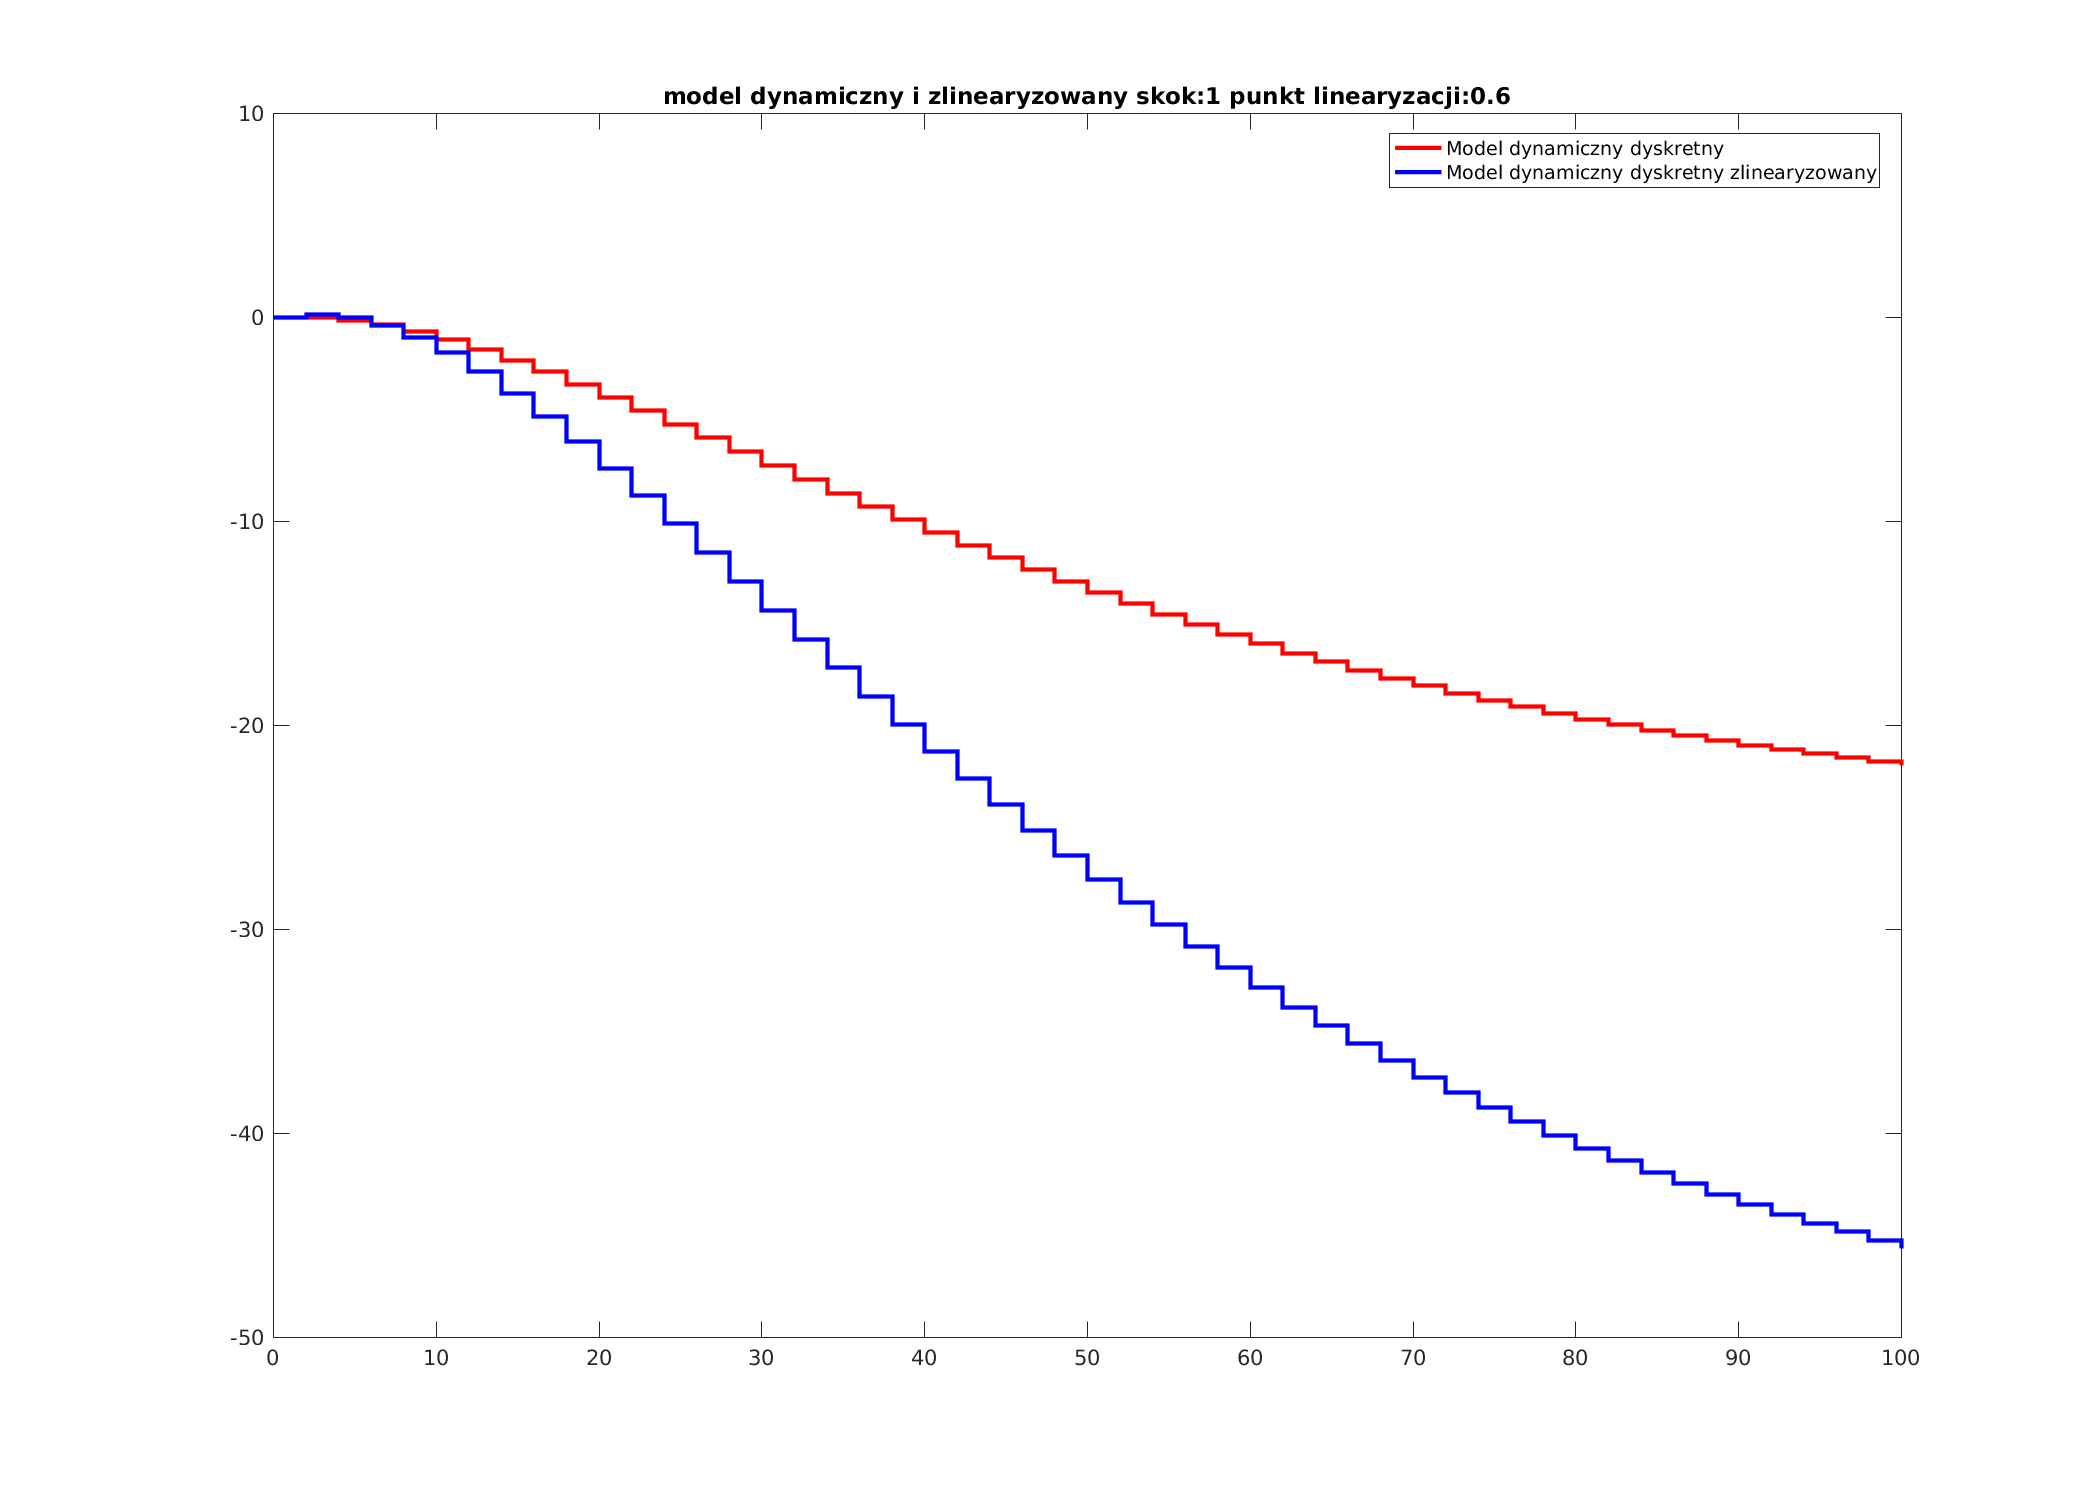
\includegraphics[scale=0.45]{916.png}
\end{figure}
\begin{figure}[H]
\centering
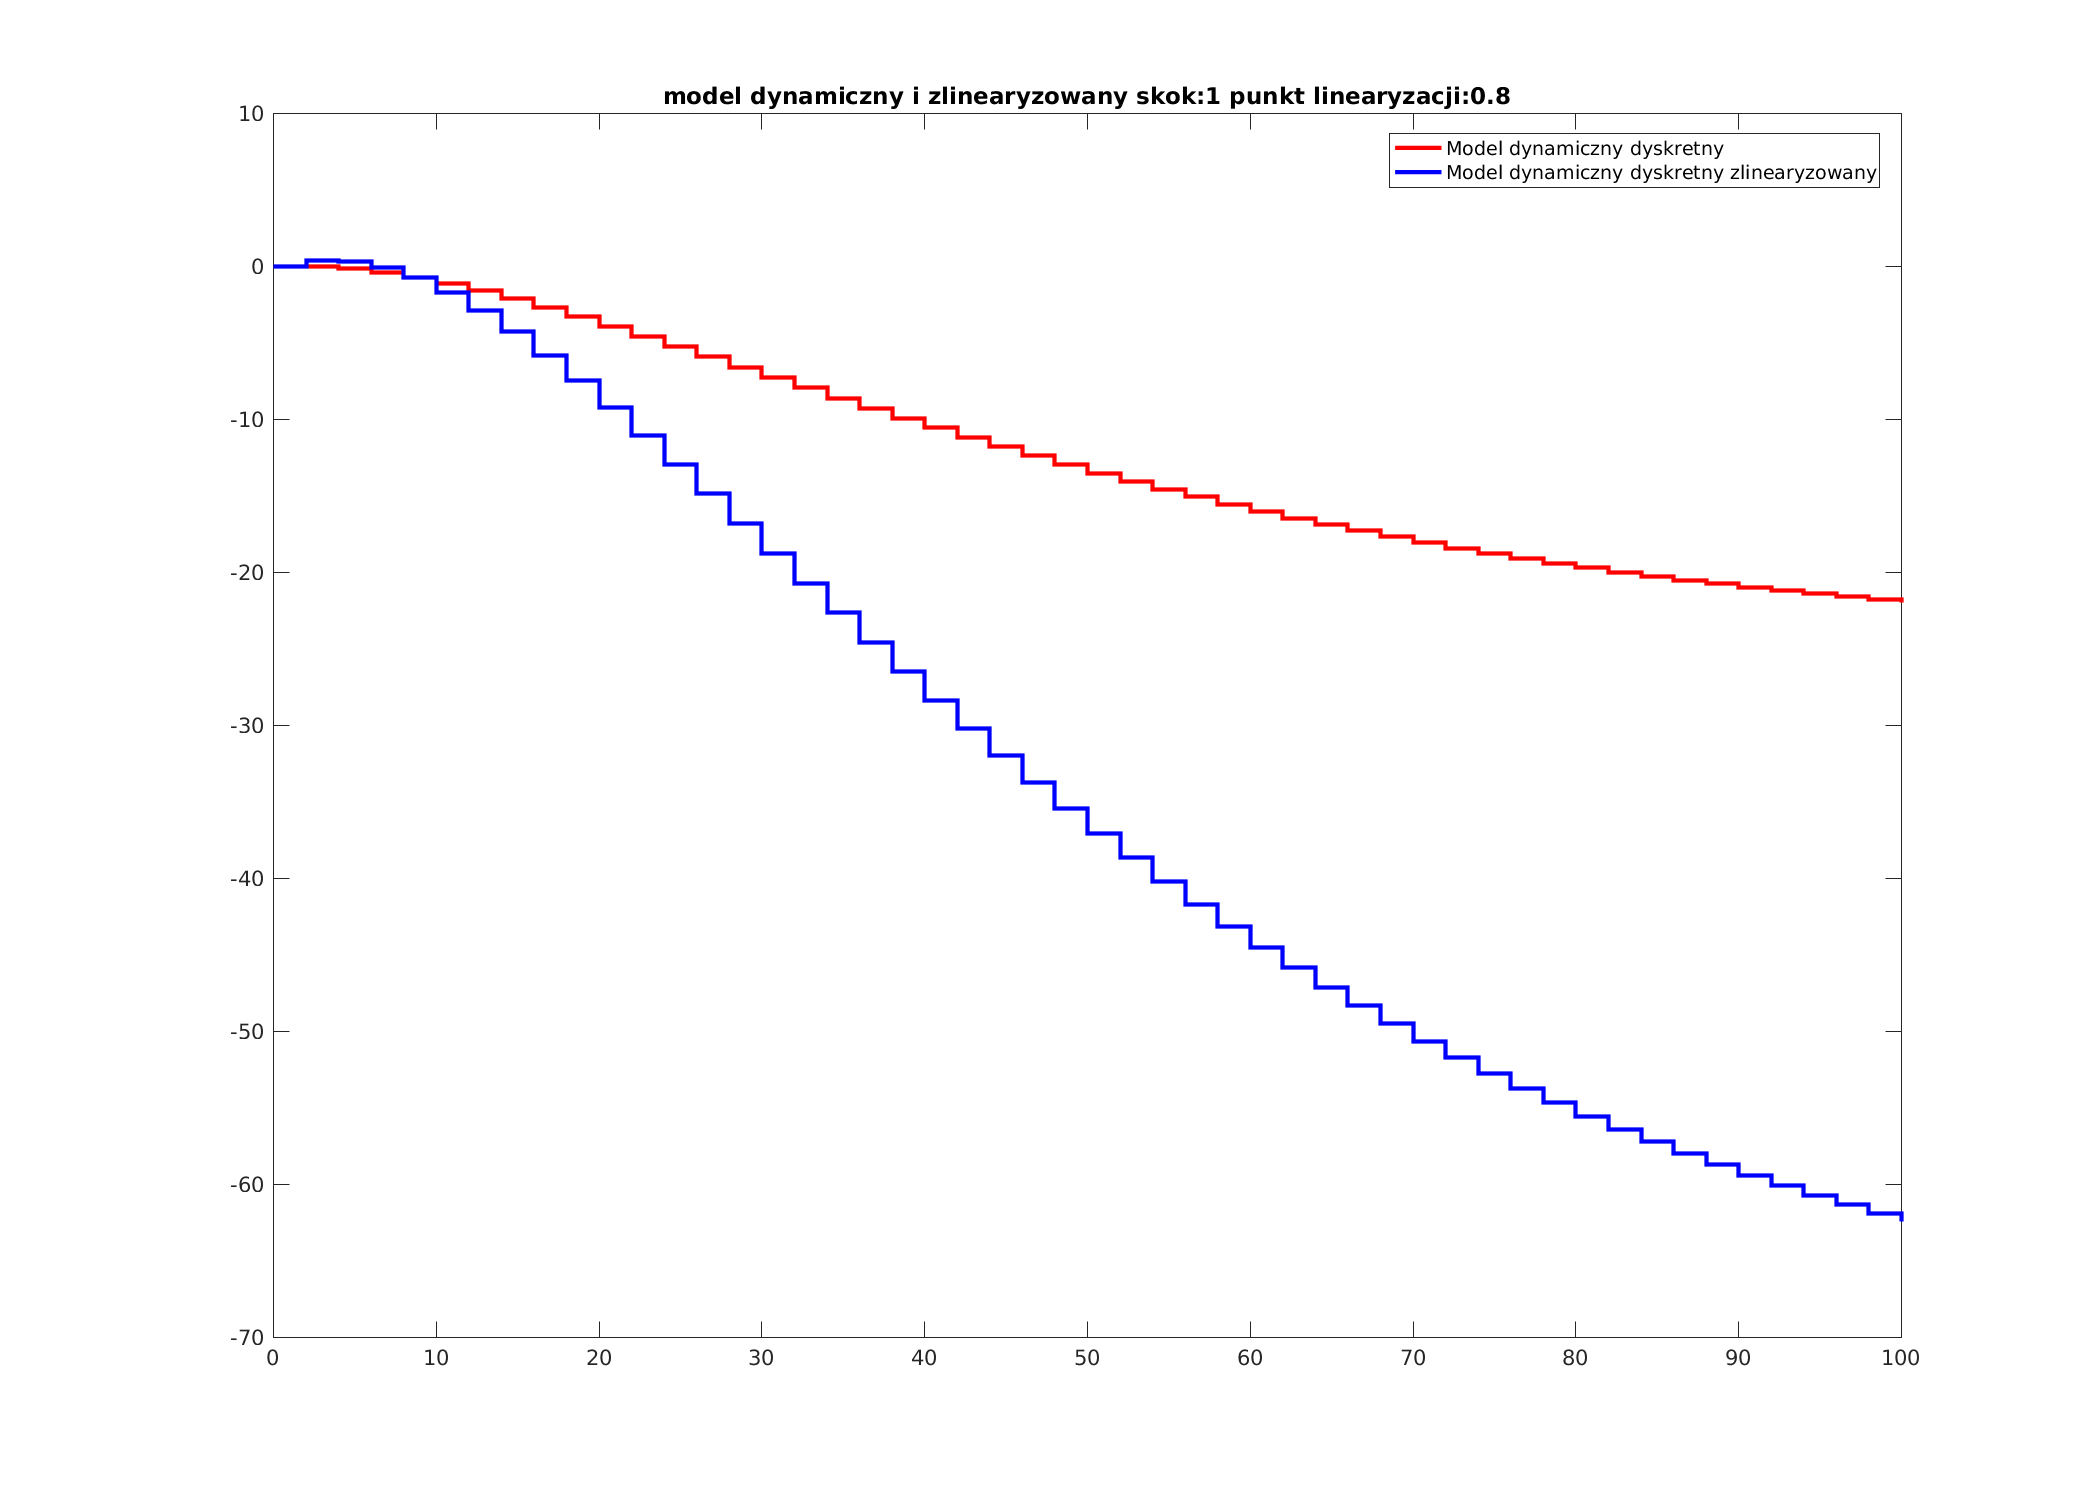
\includegraphics[scale=0.45]{918.png}
\end{figure}



\section{Transmitancja zlinearyzowanego dynamicznego modelu ciągłego}
Zlinearyzowany dynamiczny model ciągły: 
\\

$\dot{x}_1 = -\frac{T_{1}-T_{2}}{T_{1}T_{2}}x_{1}(t) +x_{2}(t)$
\\

$\dot{x}_2 = -\frac{1}{T_{1}T_{2}}x_{1}(t) + \frac{K}{T_{1}T_{2}}(\alpha_1u(t)+\alpha_2(2\overline{u}u(t) - \overline{u}^2)+ \alpha_3(3\overline{u}^2u(t)-2\overline{u}^3) + \alpha_4(4\overline{u}^3u(t) - 3\overline{u}^4))$
\\

$y(t) = x_{1}(t)$
\\
\\

\noindent Po opuszczeniu składowych stałych otrzymyjemy: 
\\

$\dot{x}_1 = -\frac{T_{1}-T_{2}}{T_{1}T_{2}}x_{1}(t) +x_{2}(t)$
\\

$\dot{x}_2 = -\frac{1}{T_{1}T_{2}}x_{1}(t) + \frac{K}{T_{1}T_{2}}u(t)(\alpha_1+2\alpha_2\overline{u}+3\alpha_3\overline{u}^2+4\alpha_4\overline{u}^3)$
\\

$y(t) = x_{1}(t)$
\\
\\

\noindent Transmitancję obliczymy ze wzoru: 

$$G(s) = C(sI-A)^{-1}B + D$$

\noindent Poszczególne macierze wynoszą: \\

$ A= \left[
        \begin{array}{cc}
         -\frac{T_1+T_2}{T_1T_2} & 1\\
         -\frac{1}{T_1T_2} & 0
         \end{array}
      \right]
      \qquad $
$ B= \left[
        \begin{array}{c}
         0\\
         \frac{K}{T_{1}T_{2}}(\alpha_1+2\alpha_2\overline{u}+3\alpha_3\overline{u}^2+4\alpha_4\overline{u}^3)
         \end{array}
      \right]
      \qquad $
$ C= \left[
        \begin{array}{cc}
         1& 0\\
         \end{array}
      \right]
      \qquad $
$$D=0$$

\noindent Korzystając z obliczeń symbolicznych pakietu matlab otrzymujemy: 
$$G(s) = \frac{K(\alpha_1+2\alpha_2\overline{u}+3\alpha_3\overline{u}^2+4\alpha_4\overline{u}^3)}{T_1T_2s^2 + (T_1+T_2)s +1}$$

\noindent Gdzie : \\

$K  = 5.5, T_1 = 7, T_2 = 7, \alpha_1 = 0.19, \alpha_2 = -0.05, \alpha_3 = -0.95, \alpha_4 = -0.45,\overline{u}$ - punkt linearyzacji 
\\

\section{Wzmocnienie statyczne transmitancji}
$$K_{stat} = \lim_{s \rightarrow 0} G(s) = K(\alpha_1+2\alpha_2\overline{u}+3\alpha_3\overline{u}^2+4\alpha_4\overline{u}^3)$$
\subsection{Wykres wzmocnienia statycznego w zależności od punktu linearyzacji}
\begin{figure}[H]
\centering
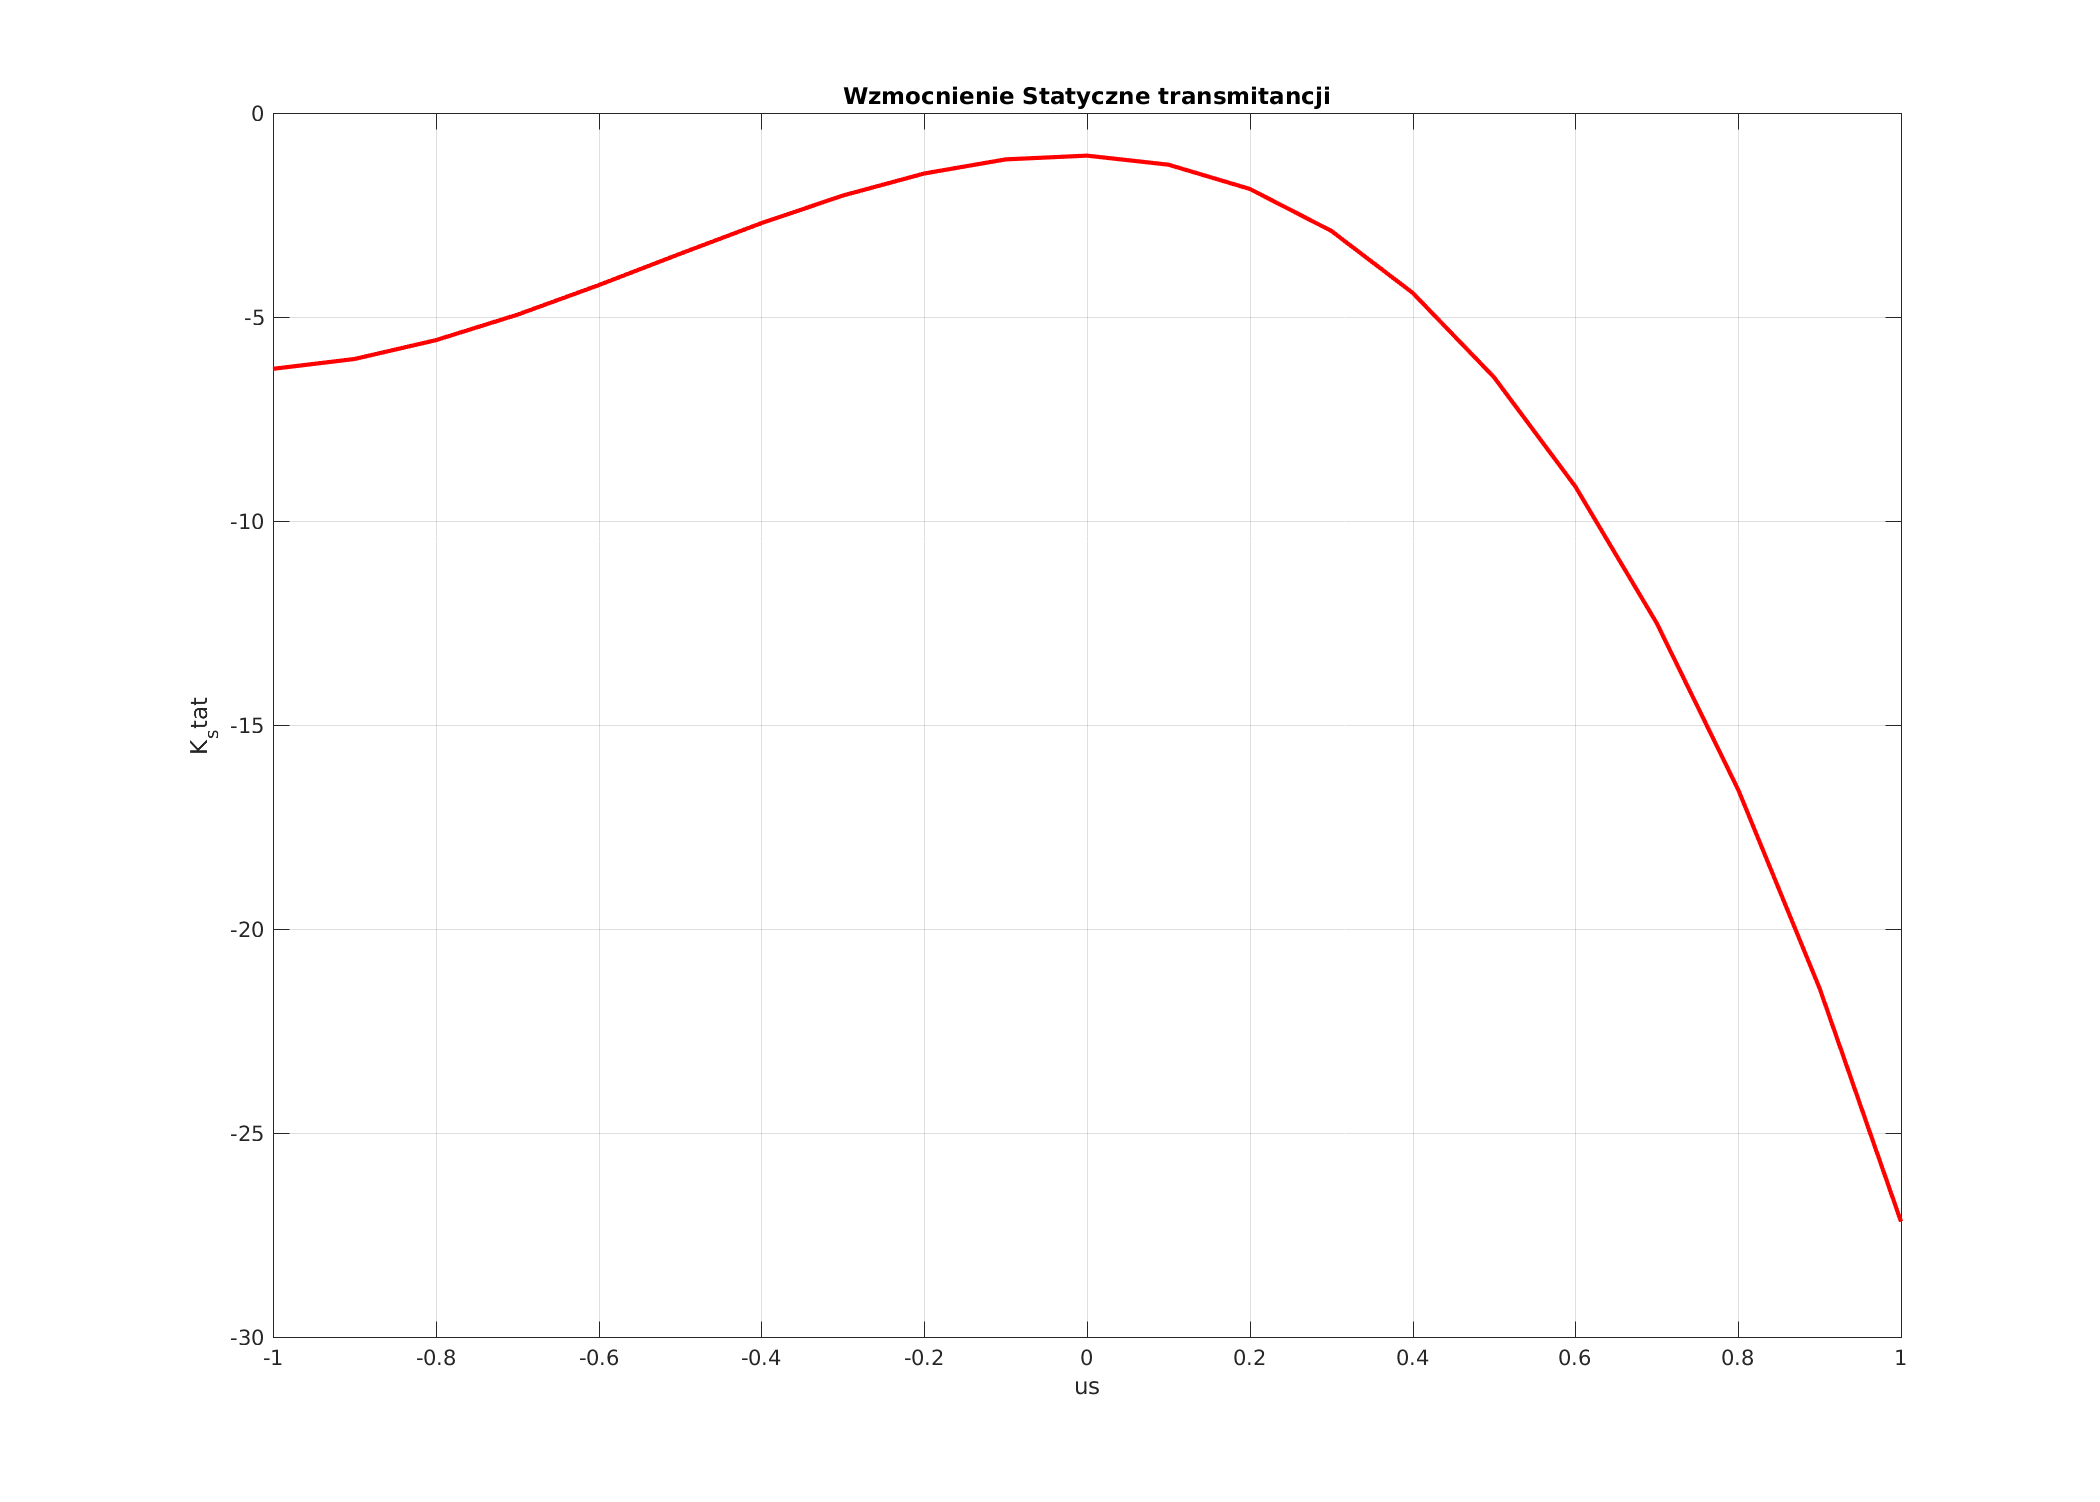
\includegraphics[scale=0.5]{stat.png}
\caption{Wykres wzmocnienia statycznego transmitancji w zależności od punktu linearyzacji}
\end{figure}

\section{Sprawdzenie dla modelu ststycznego i dynamicznego}
Wzmocnienie statyczne transmitancji odpowiada wzmocnieniu dynamicznego układu zlinearyzowanego, którego odpowiedzi obserwowaliśmy w zadaniu 9. Jak wynika z wykresu wzmocnienia statycznego, dla punktu linearyzacji równego 0.25, K przyjmuje wartość $\approx -2.5$ i taką samą wartość przyjmuje sygnał na wyjściu zlinearyzowanego modelu dla punktu linearyzacji równego 0.25 dla sygnału sterującego będącego skokiem jednostkowym do wartości 0.25. Tak samo jest w przypadku innych, wcześniej badanych, punktów linearyzacji. Potwierdza to zgodność wzmocnienia statycznego transmitancji i wzmocnienia dynamicznego układu zlinearyzowanego. Wzmocnienie dynamiczne układu zlinearyzowanego zostało odczytane z wykresu jako wartość funkcji w stanie ustalonym. Dla niektórych wartości sterowania niemożliwe było odczytanie wzmocnienia układu ze względu na zbyt krótki horyzont czasowy symulacji. 



\end{document}